The BDT is trained with scikit-learn package~\cite{scikit-learn}. The classifier has 200 trees and employs the AdaBoost method. The background sample is taken from data events with $80~\GeV < \Mbb <100$~\GeV~and $150~\GeV<\Mbb<190$~\GeV~and contains approximately 690k events for the \fourcentral channel and 90k events for the \twocentral channel. The signal contamination in this region is negligible.  The $Z$ contribution to the low-mass sideband is not explicitly accounted for due to its small size (see Tables~\ref{tab:cutflow_4cen} and~\ref{tab:cutflow_2cen} for the number of events of each type passing pre-selection).  As will be shown in Figure~\ref{fig:BDTResponse},  the BDT response of the QCD-produced \zjets~ sample is very similar to the background samples. 

The signal sample is the VBF Monte Carlo simulated dataset and contains 10k events for the \fourcentral channel and 2k events for the \twocentral channel.  Half of the signal and background samples are used for training and the other half are used for validation.  No MC event weights are used in the training.  

The following variables are used for training:
\begin{enumerate}
\item $M_{\rm JJ}$, the invariant mass of the VBF jet pair. 
\item $p_{\rm T,JJ}$, the transverse momentum of the VBF jet pair. 
\item $\cos{\theta}$, cosine of the polar angle of the cross product of the momenta of the VBF jets in the Higgs boson's rest frame.
%\item $\Delta \eta_{\rm JJ}$, the pseudo-rapidity difference between VBF jets.
\item $Max (\eta)$, the maximum between the absolute values of the pseudo-rapidity of the VBF jets: $Max (\eta) \equiv max( |\eta_{J1}|, |\eta_{J2}| )$
\item $\eta* = \frac{1}{2}( |\eta_{\rm J1}| + |\eta_{\rm J2}| - |\eta_{\rm B1}| - |\eta_{\rm B2}|)$, average pseudo-rapidity difference between VBF and signal jets.
%\item $H_{\rm T}$, scalar sum of jet \pT; The jets are required to have \pT$>20$\GeV~and not selected as signal or VBF jets.
\item $min\Delta R$(J1), minimum angular separation between the leading VBF jet and its closest jet. 
\item $min\Delta R$(J2), minimum angular separation between the sub-leading VBF jet and its closest jet. 
\item $N_{\rm Trk}($J1$)$, quark/gluon tagger for the leading VBF jet.
\item $N_{\rm Trk}($J2$)$, quark/gluon tagger for the sub-leading VBF jet.
\item $p_{T}$ balance, the ratio of vectorial and scalar sum of signal and VBF jets \pT,  $\frac{ \overrightarrow{p_{T}}(J1)+\overrightarrow{p_{T}}(J2)+\overrightarrow{p_{T}}(B1)+\overrightarrow{p_{T}}(B2) }{ p_{T}(J1)+p_{T}(J2)+p_{T}(B1)+p_{T}(B2)  }$
\item $\Delta M_{\rm JJ}$, the difference between largest invariant mass calculated using all jet pairs and only VBF jet pair. 

\end{enumerate}


The distributions of all input variables for each channel are shown in Figures~\ref{fig:BDTInputs2cen} and Figures~\ref{fig:BDTInputs4cen}. As shown in Figure~\ref{fig:BDTInputsCor}, most variables have a small correlation factor of less with \Mbb.  The most correlated variables with \Mbb is $\Delta M_{\rm JJ}$. Further studies of the correlation with \Mbb and the BDT variables, the relative importance of each variable in the BDT, and a 3-fold validation test are shown in Appendix~\ref{sec:app-bdt}. From these studies we conclude that the BDT discriminant is not significantly correlated with \Mbb with the exception of very high BDT scores.

The BDT response for  the signal and background training and validation samples for both channels is shown in Figure~\ref{fig:BDTResponse}.    In the \fourcentral channel the VBF \Hbb BDT distribution peaks at 0.03.  The background sample peaks at -0.02.  In the \twocentral channel the VBF \Hbb distribution has a single broad peak at 0.05 and the background peaks at -0.02. Good agreement is seen between the training and validation datasets, indicating that the BDT training is adequate.  A Kolmogorov-Smirnov test is used to check the compatibility between the training and validation datasets.  The \twocentral channel has a 0.52 $p$-value for the observed agreement in the background sample and 0.58 $p$-value for the signal sample. The \fourcentral channel has a $p$-value of 0.95 for the background and $p$-value of 0.99 for the signal.  Figure~\ref{fig:BDTResponse} also shows the compatibility of the BDT shapes for all samples considered in this analysis.  The ggF Higgs production and QCD-produced \zjets ~ samples have a nearly identical response to the background sample in the \fourcentral channel.  In the \twocentral channel these samples have a slightly higher average BDT score than the background distribution.  The EWK \zjets ~ production has a most probable BDT score which is higher than the background samples, but less than the VBF \Hbb sample in both cases. 

To constrain the background estimate, we define control regions to have less than 1\% (3\%) VBF signal acceptance for \twocentral(\fourcentral) channel. Around 20.4(32.7)\% of the \fourcentral(\twocentral) background events pass this cut. To select the optimal signal regions in the \fourcentral channel, we scan the VBF signal events in the top forty percentile of BDT scores to maximize the sum of $\frac{S}{\sqrt{B}}$ in the Higgs mass window (100~\GeV$<\Mbb<$140~\GeV).  The number of signal events, $S$, is the sum of the VBF and $ggF$ events in the considered BDT range.  The number of background events is estimated by scaling the number of events in the Higgs mass window of the 0-tag sample by the ratio of the events in the sidebands for the 2- and 0-tag samples. Specifically $B$ is given by $N_{\rm 0~tag, mw}\times \frac{N_{\rm 2~tag, sb}}{N_{\rm 0~tag, sb}}$ where  $N_{\rm 0~tag, mw}$ is the number of events from the 0-tag sample in the Higgs mass window, and $N_{\rm 2(0)~tag, sb}$ is the number of events in the side-band regions for 2(0)-tag sample. For the \twocentral channel, we cut the BDT scores to make three signal regions such that they contain the top 30\%, 30\%-40\% and 40\%-60\% VBF signal.   These regions are chosen such that $S/\sqrt{B}$ is high and the \Mbb{} distribution is well-behaved in the low-mass sideband as the BDT score correlation with\ Mbb{} is non-linear for very high BDT scores.  See Appendix~\ref{sec:app-bdt} for details on the correlation between \Mbb, BDT score and \pTbb. 

The definition of the signal and control regions, the yields of each processes and the estimation of sensitivity are listed in Tables~\ref{tab:BDTReg2cen} and ~\ref{tab:BDTReg4cen}. 
 
\begin{figure}[htbp]
  \centering
 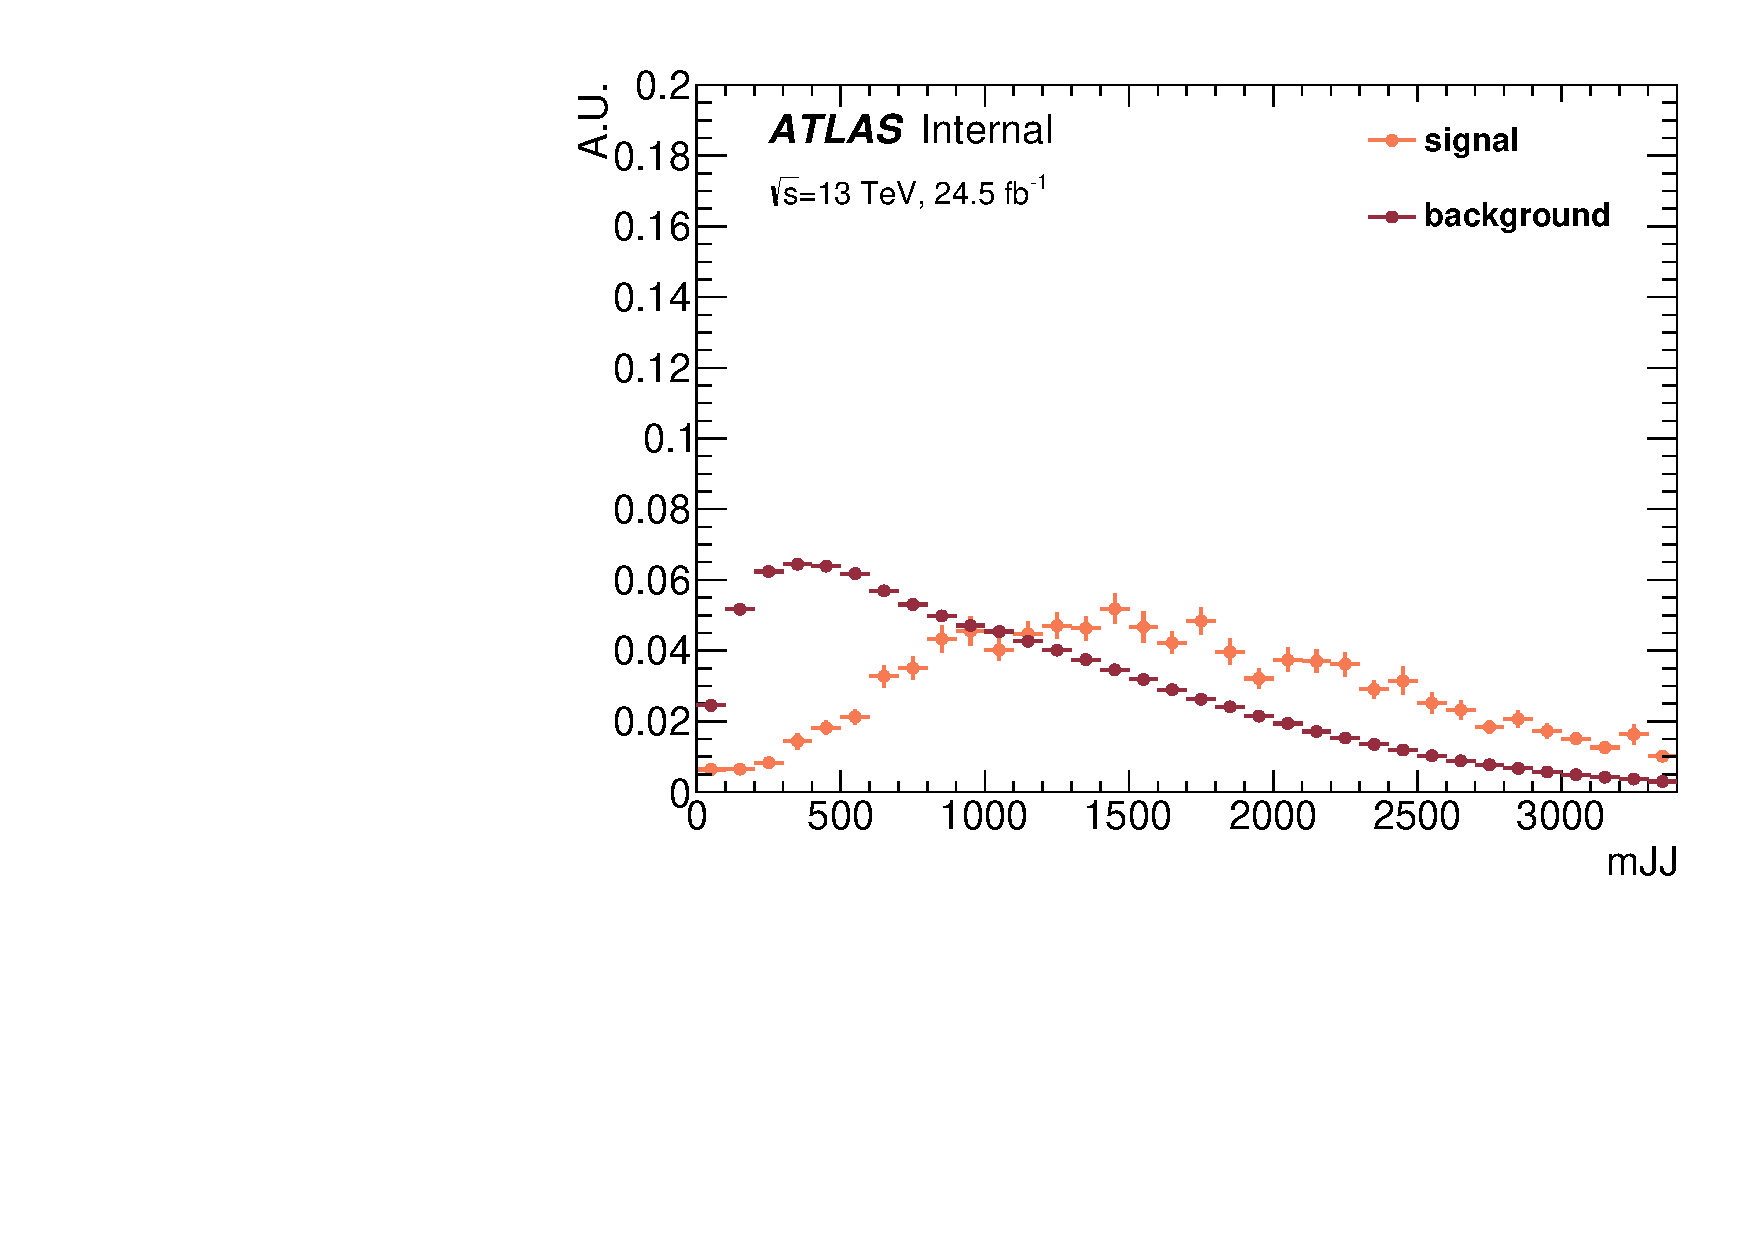
\includegraphics[width=0.3\textwidth]{figures/BDT_mJJ_2cen.pdf}
 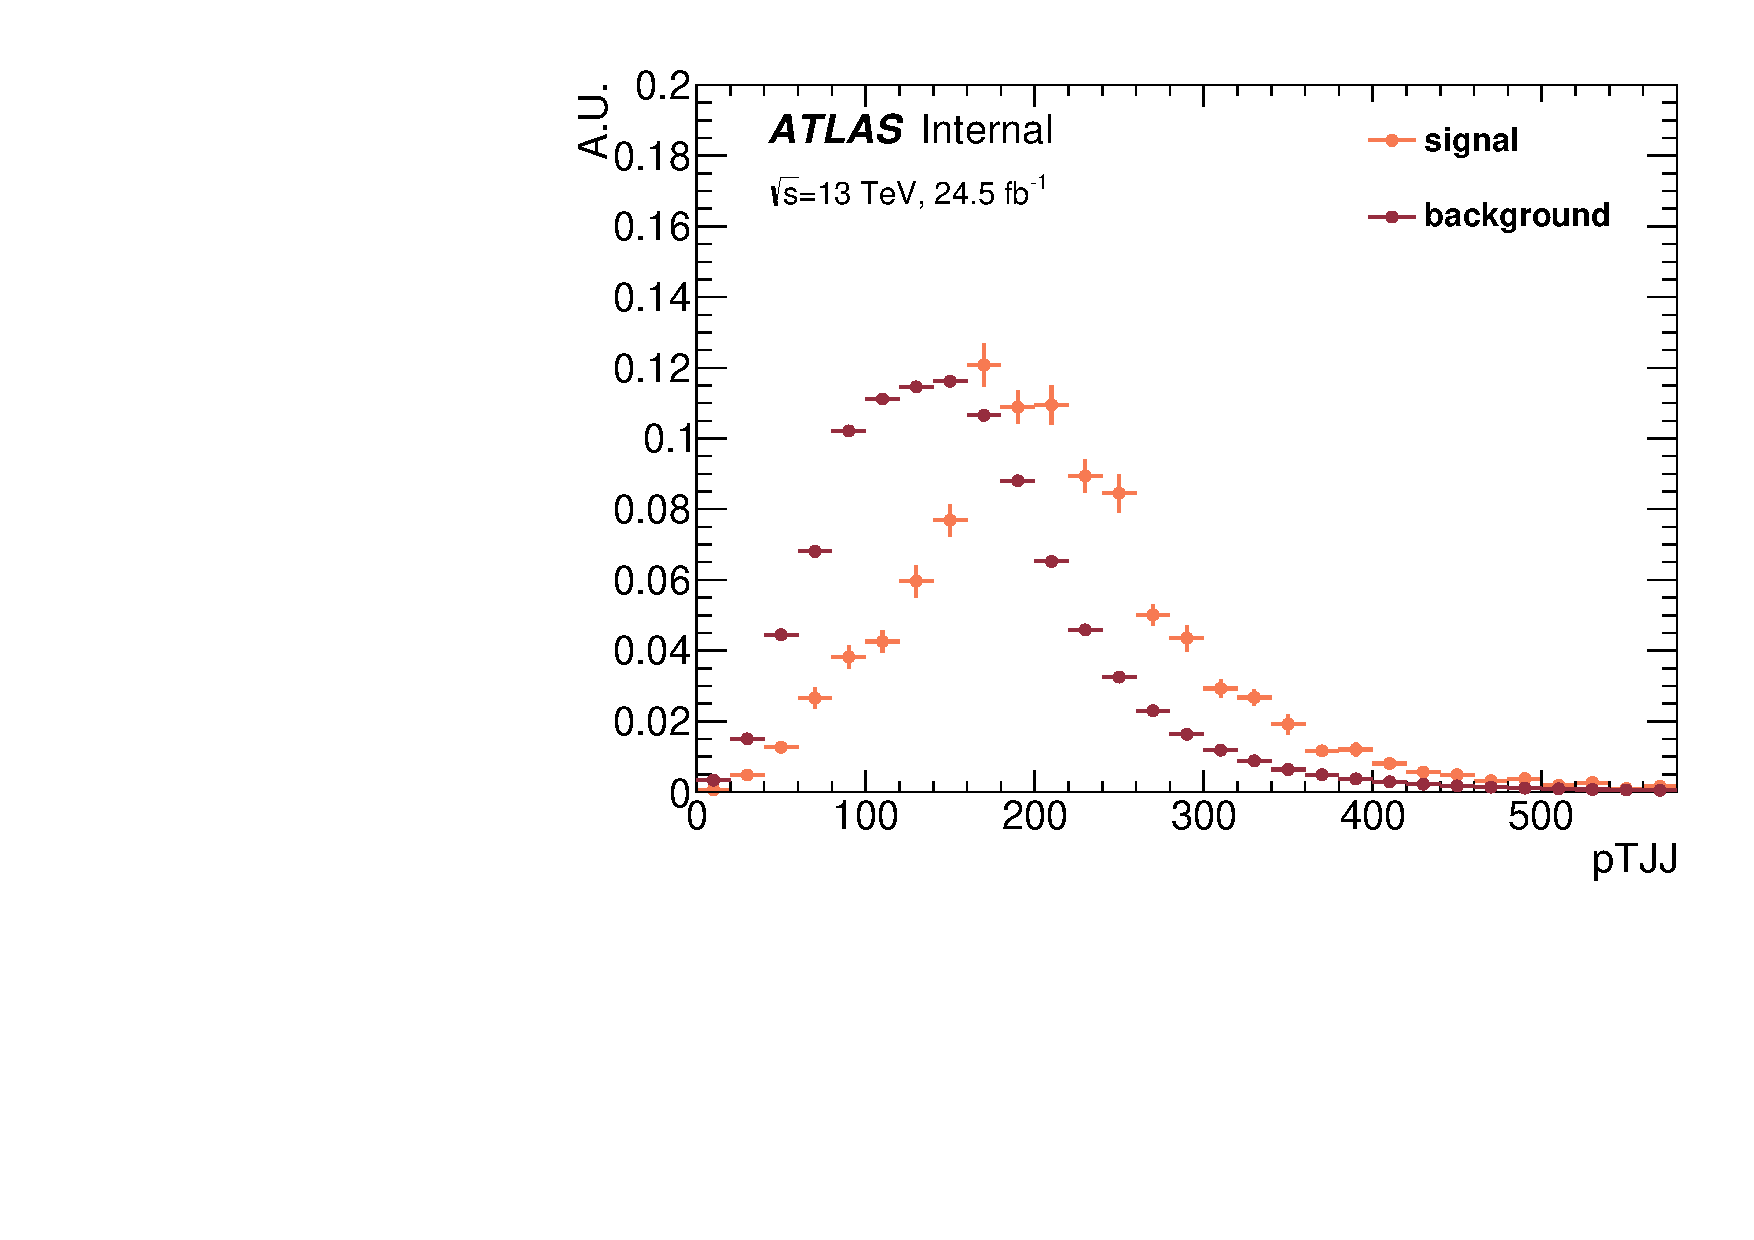
\includegraphics[width=0.3\textwidth]{figures/BDT_pTJJ_2cen.pdf}
 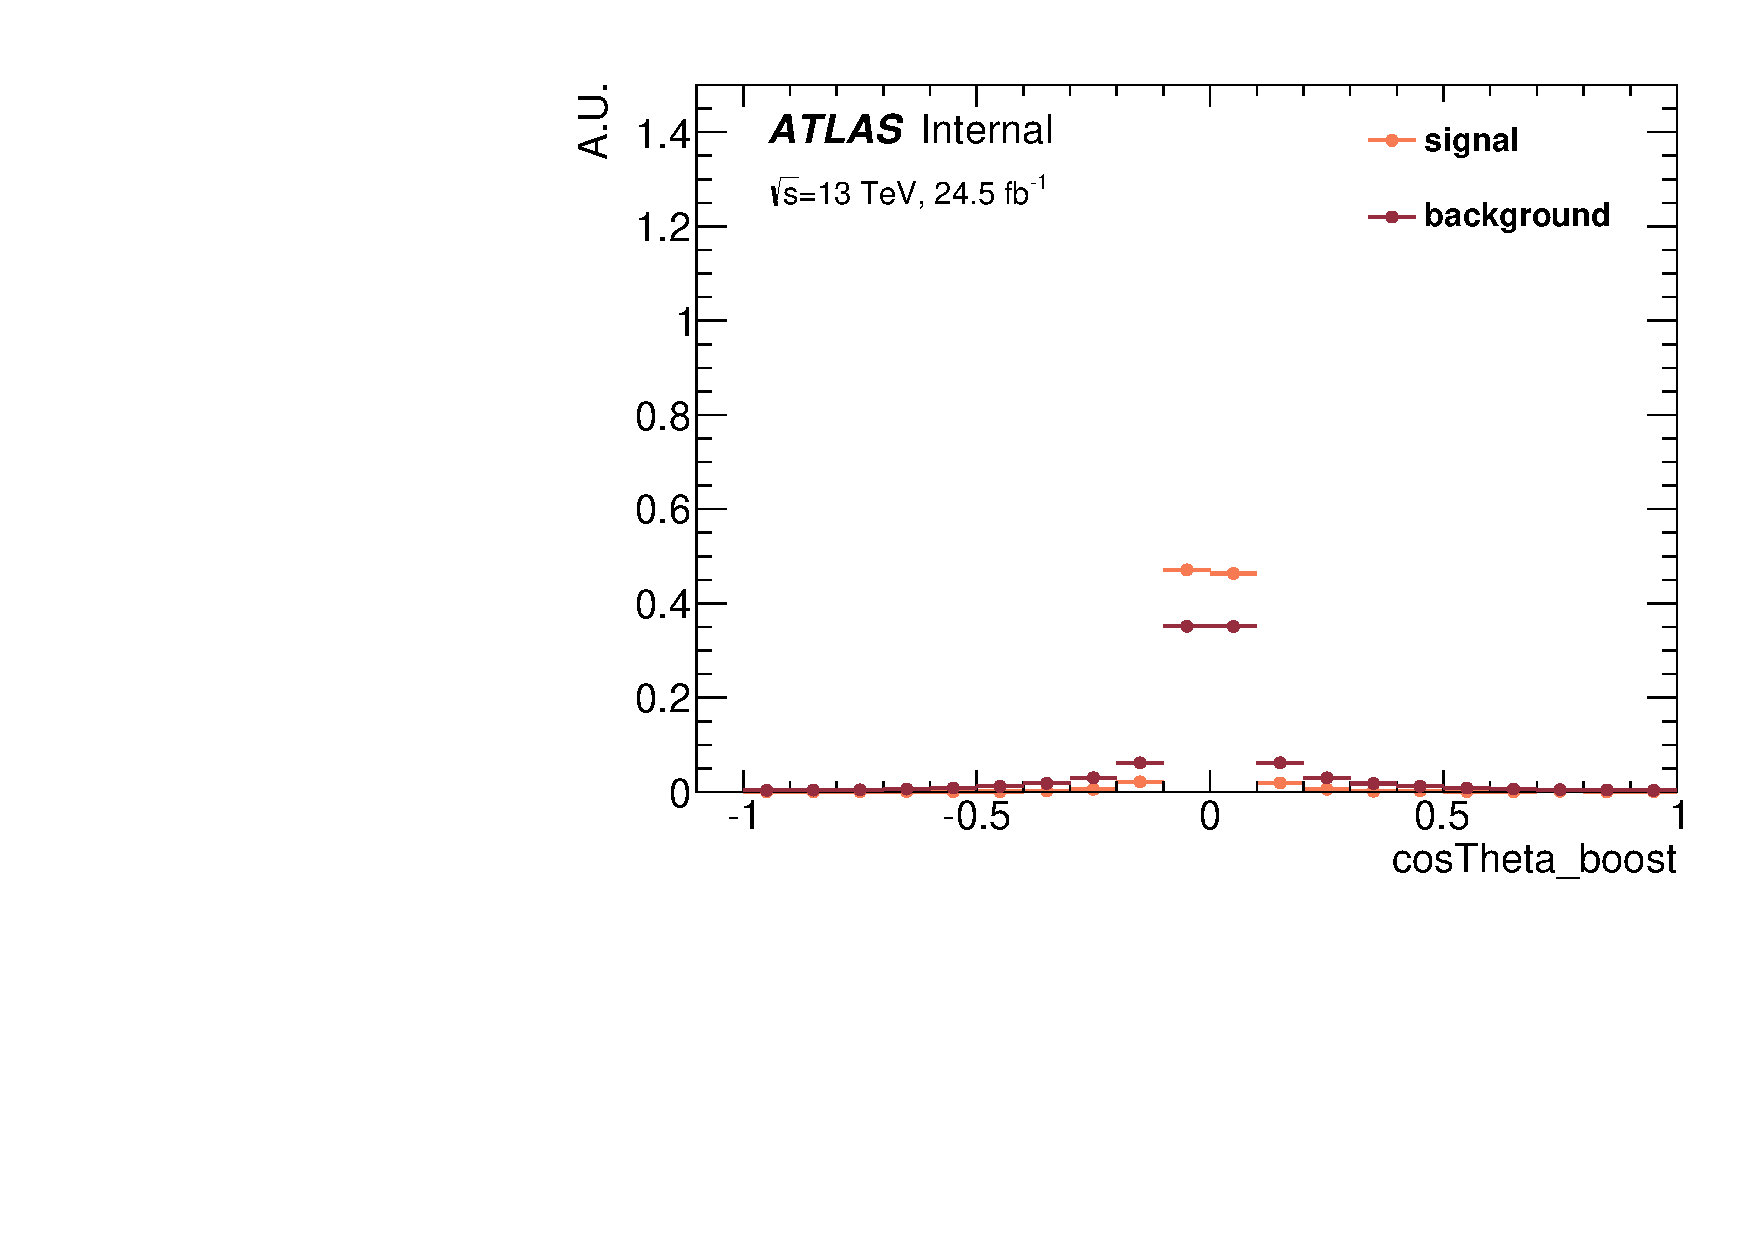
\includegraphics[width=0.3\textwidth]{figures/BDT_cosTheta_2cen.pdf}\\
% 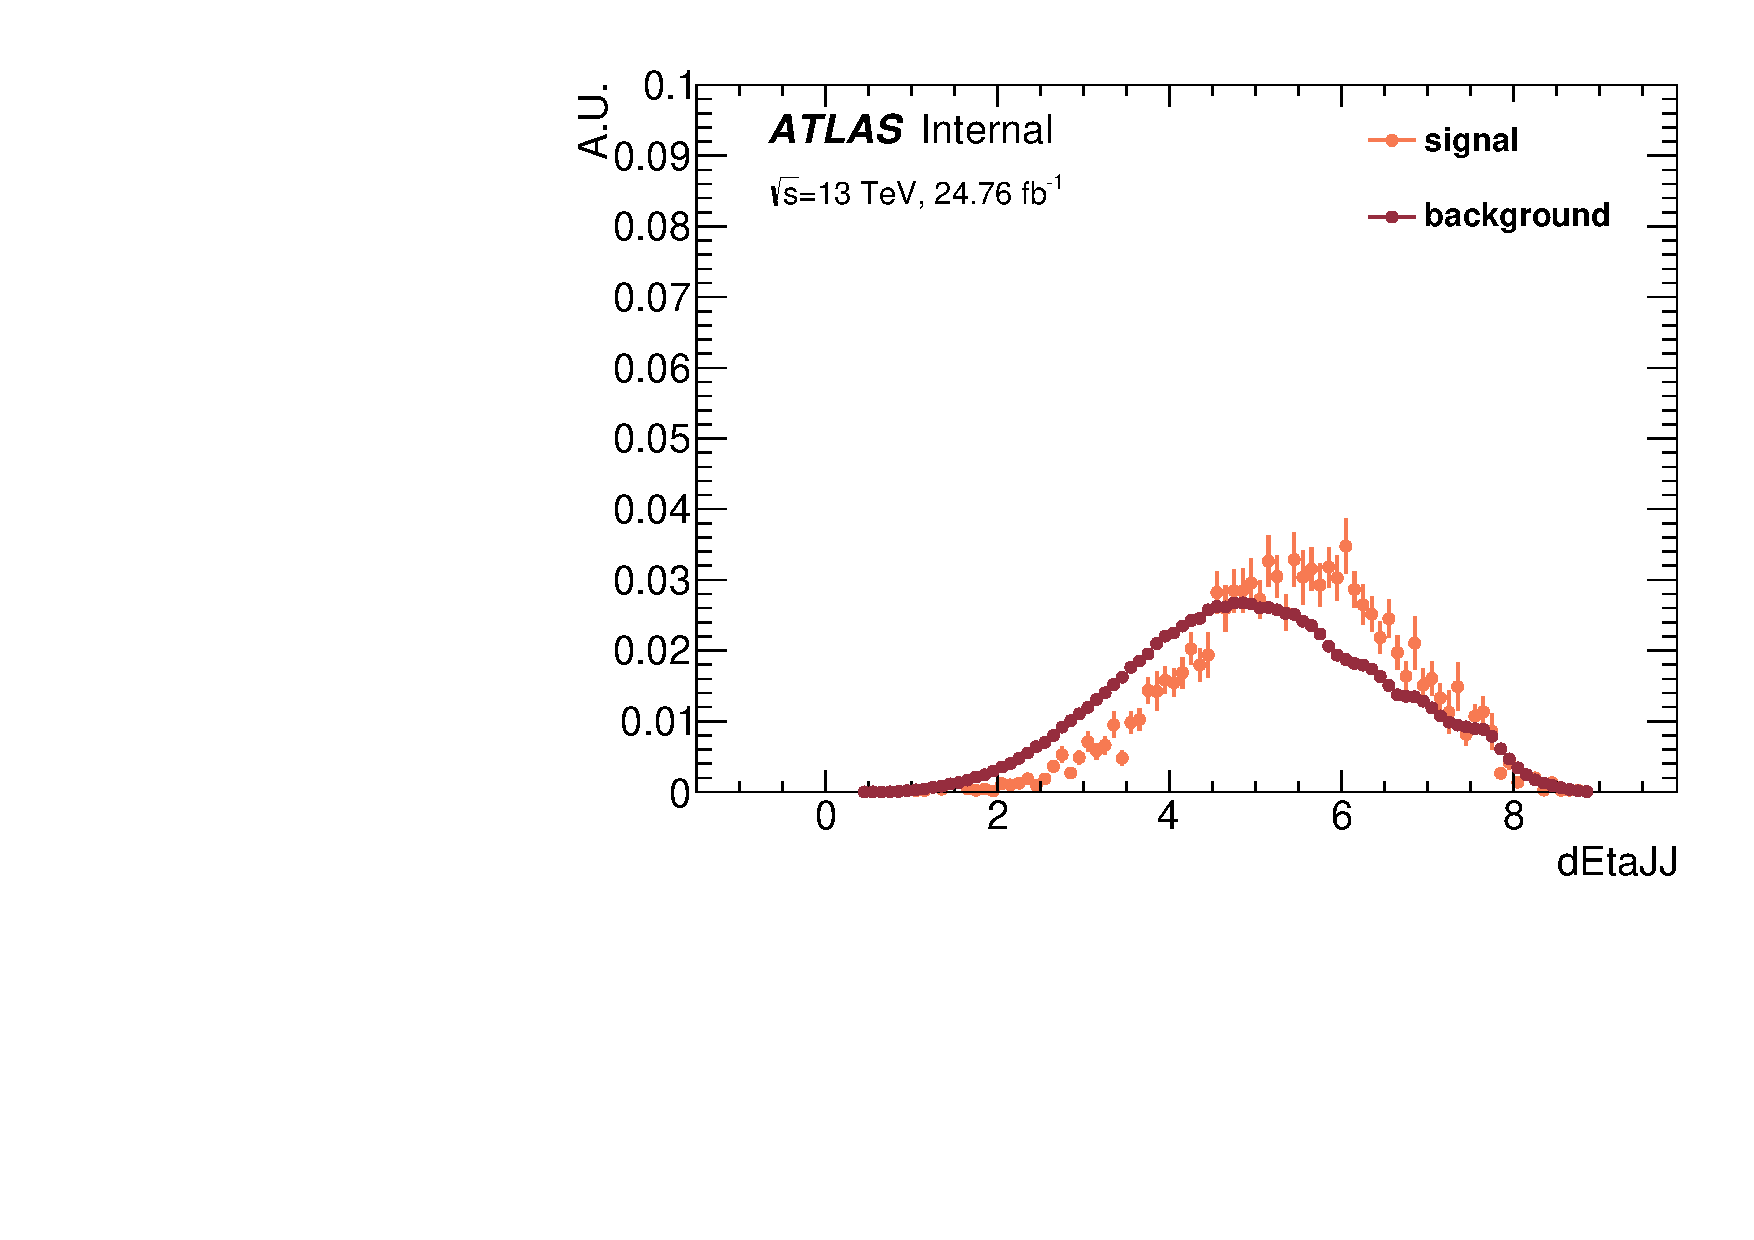
\includegraphics[width=0.3\textwidth]{figures/BDT_dEtaJJ_2cen.pdf}
 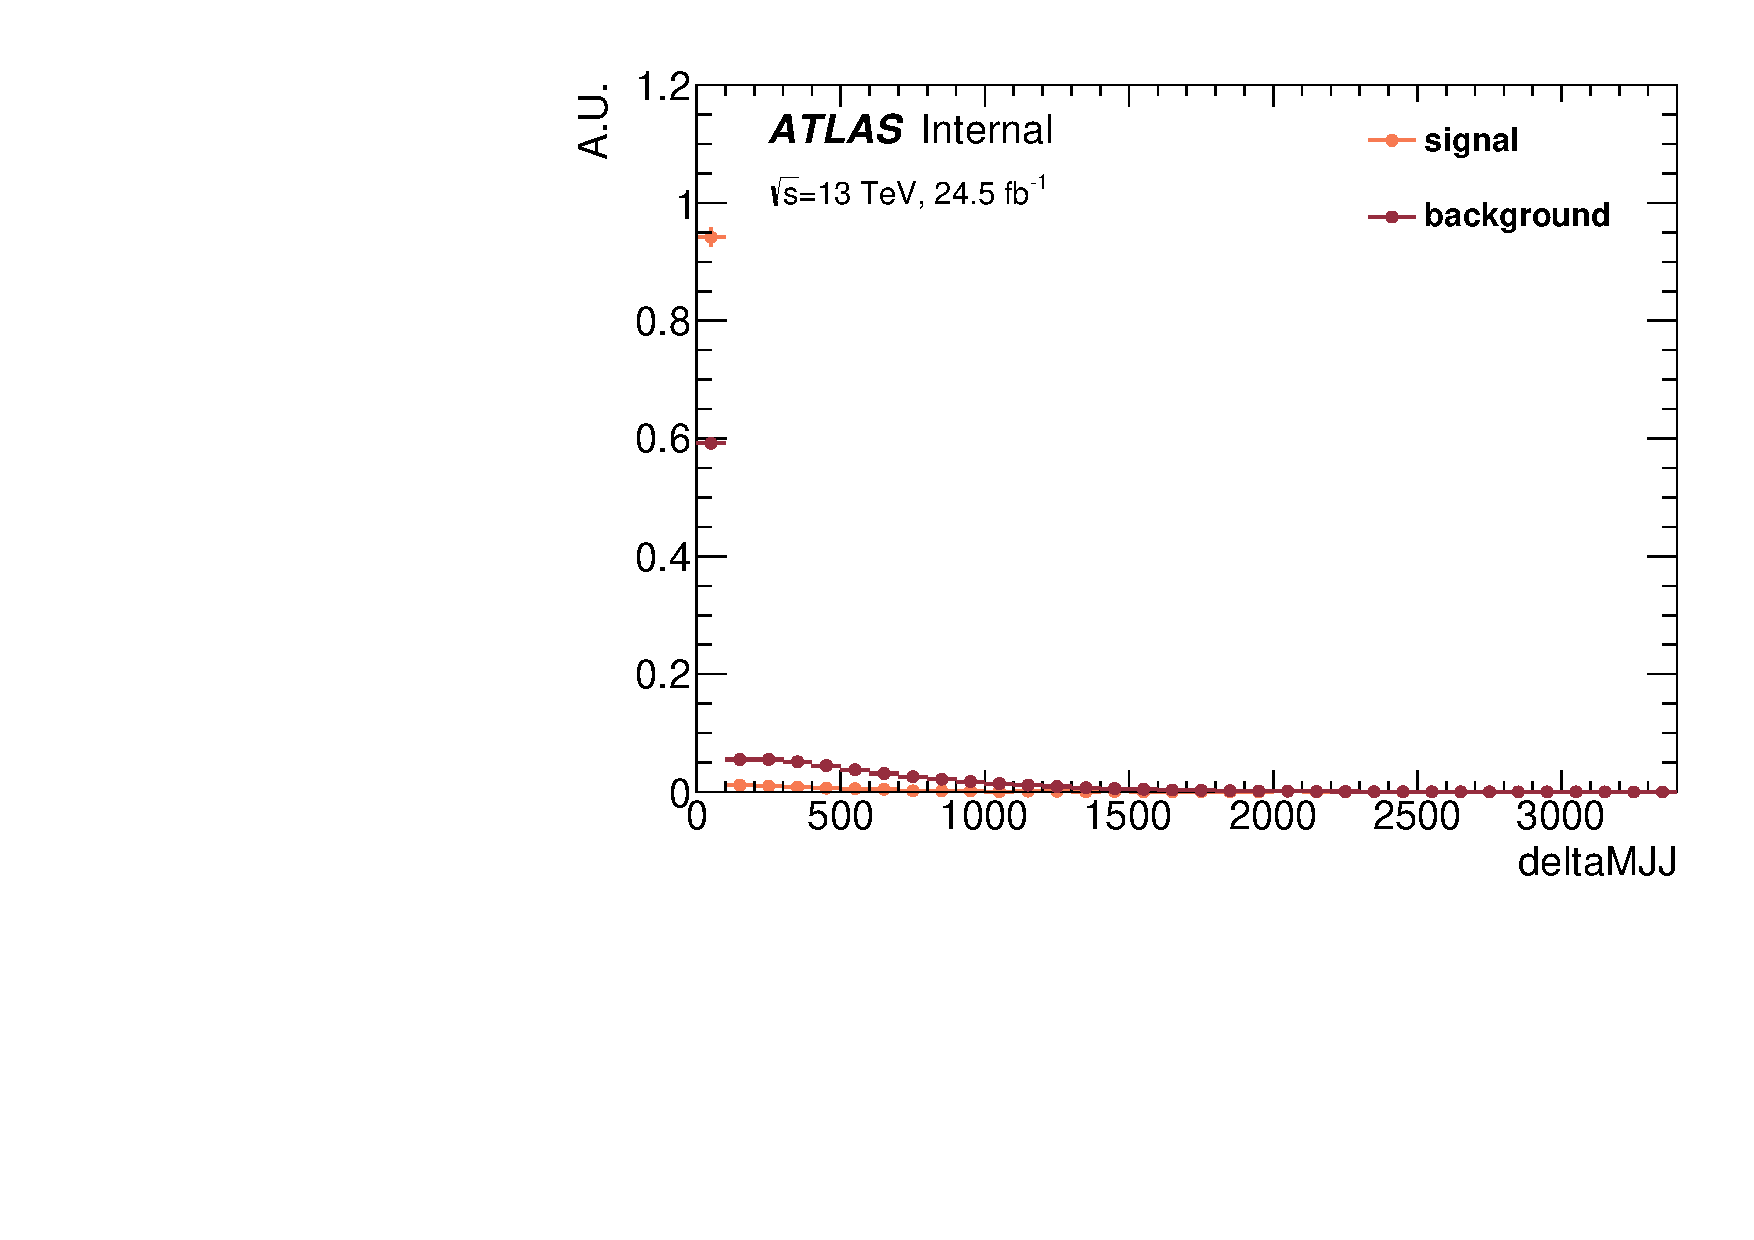
\includegraphics[width=0.3\textwidth]{figures/BDT_deltaMJJ_2cen.pdf}
 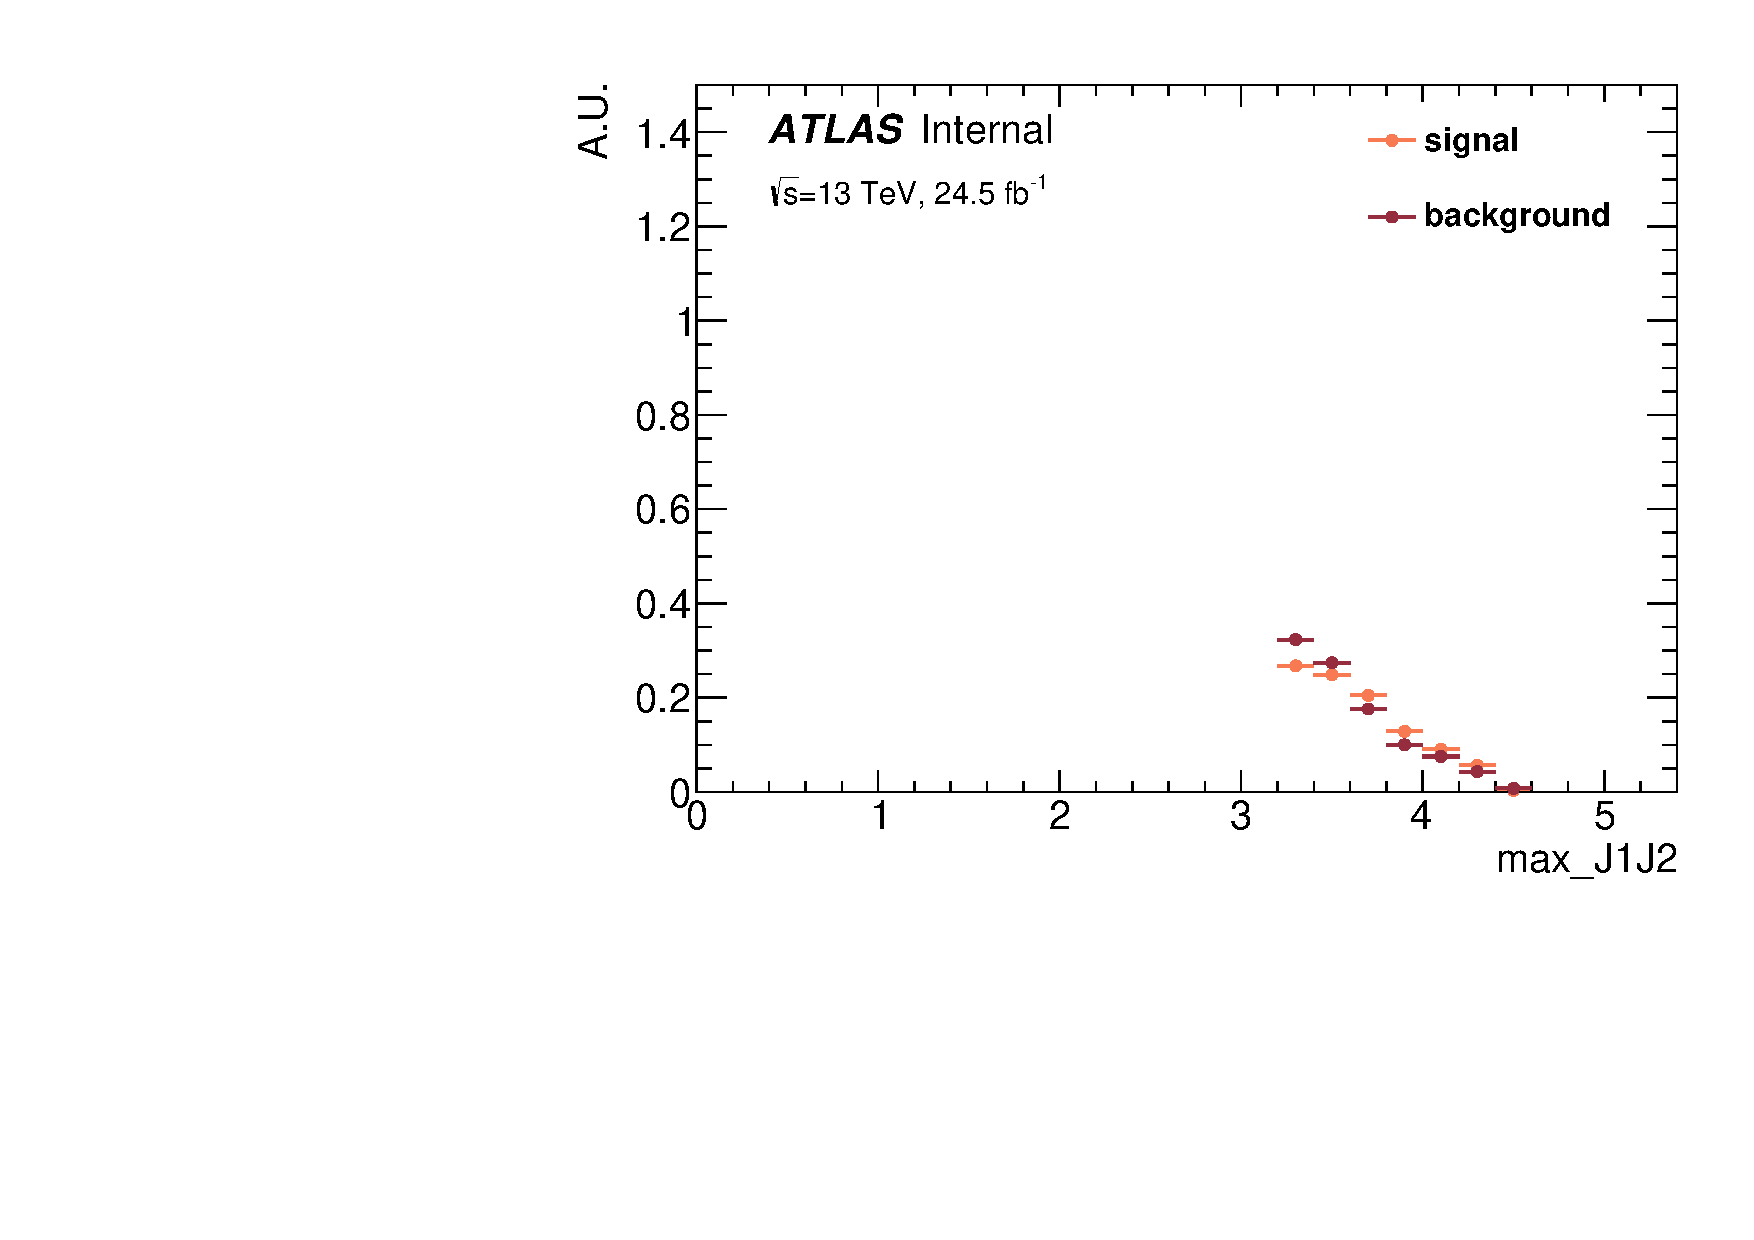
\includegraphics[width=0.3\textwidth]{figures/BDT_maxJ1J2_2cen.pdf}
 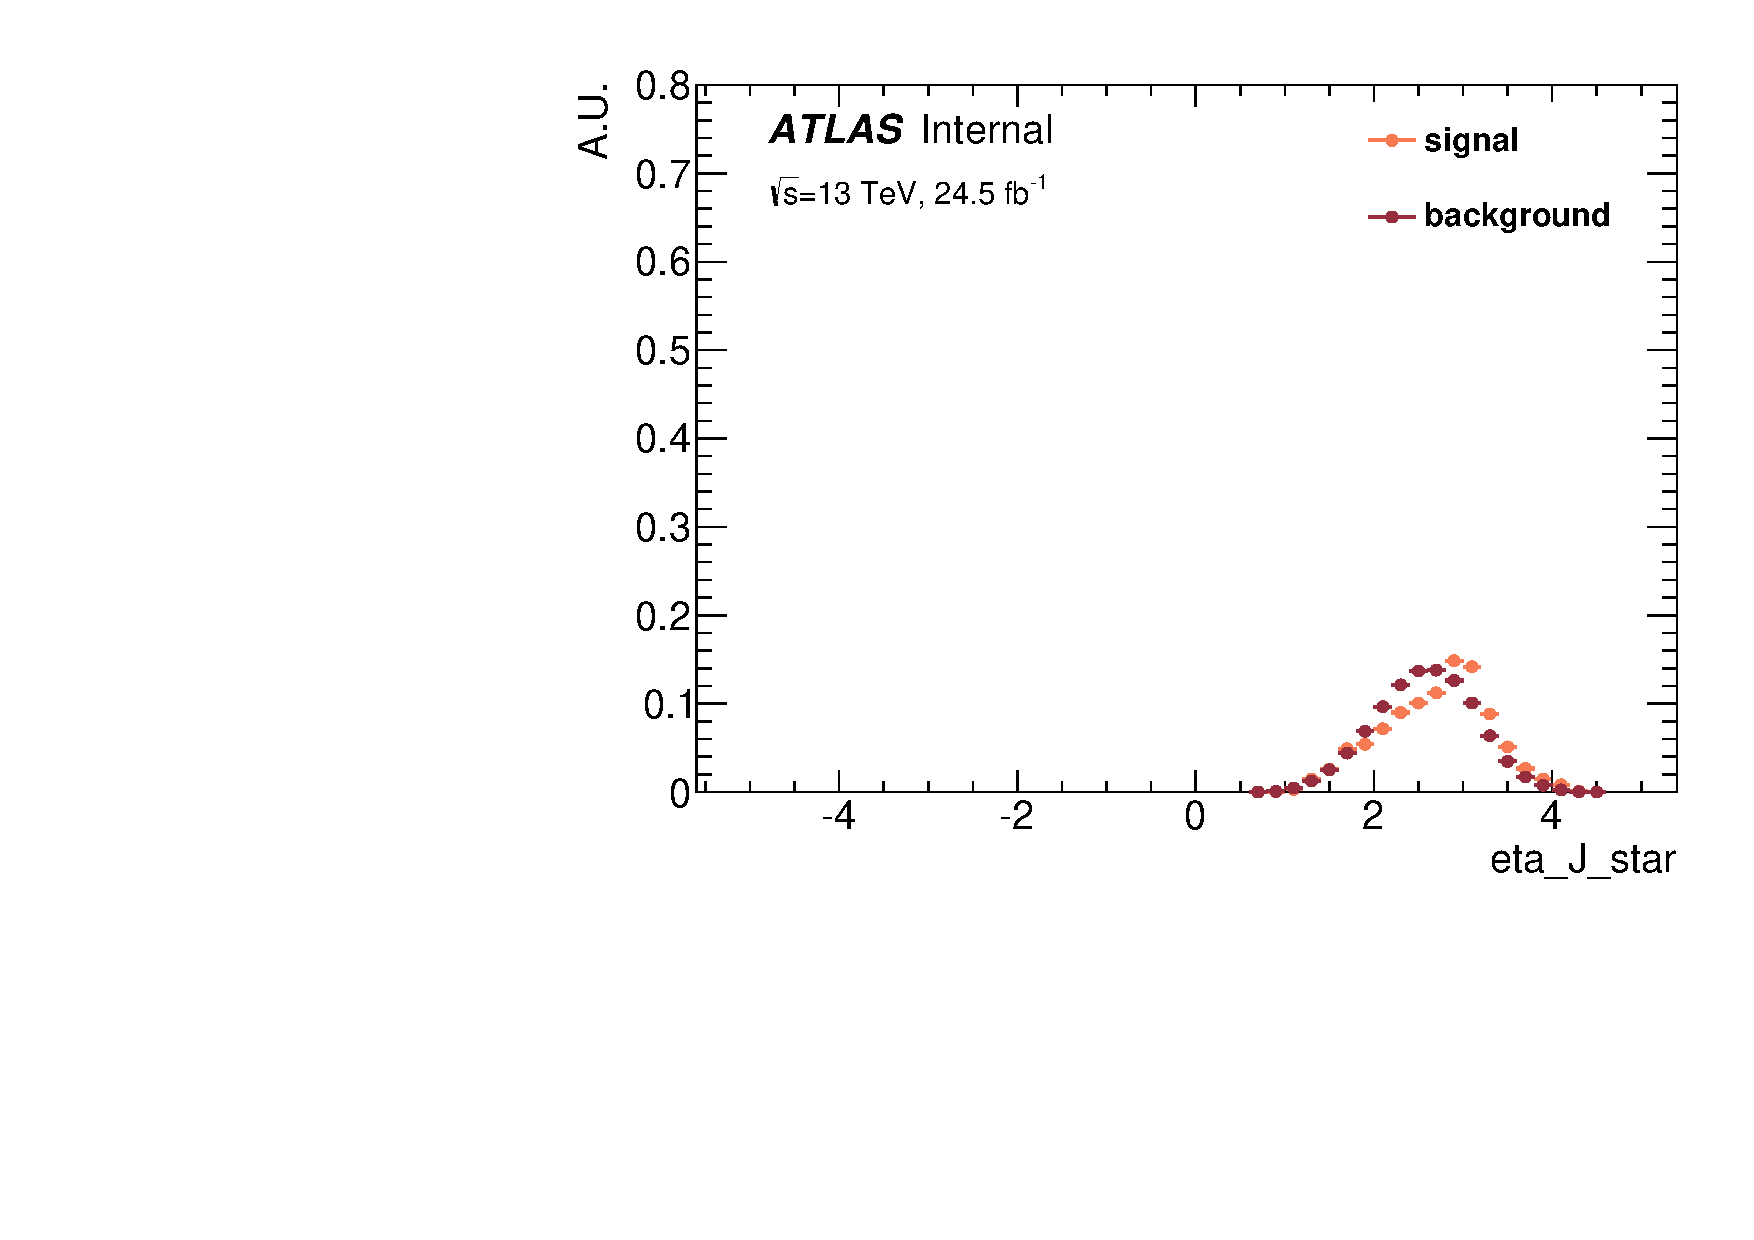
\includegraphics[width=0.3\textwidth]{figures/BDT_etaJstar_2cen.pdf}\\
 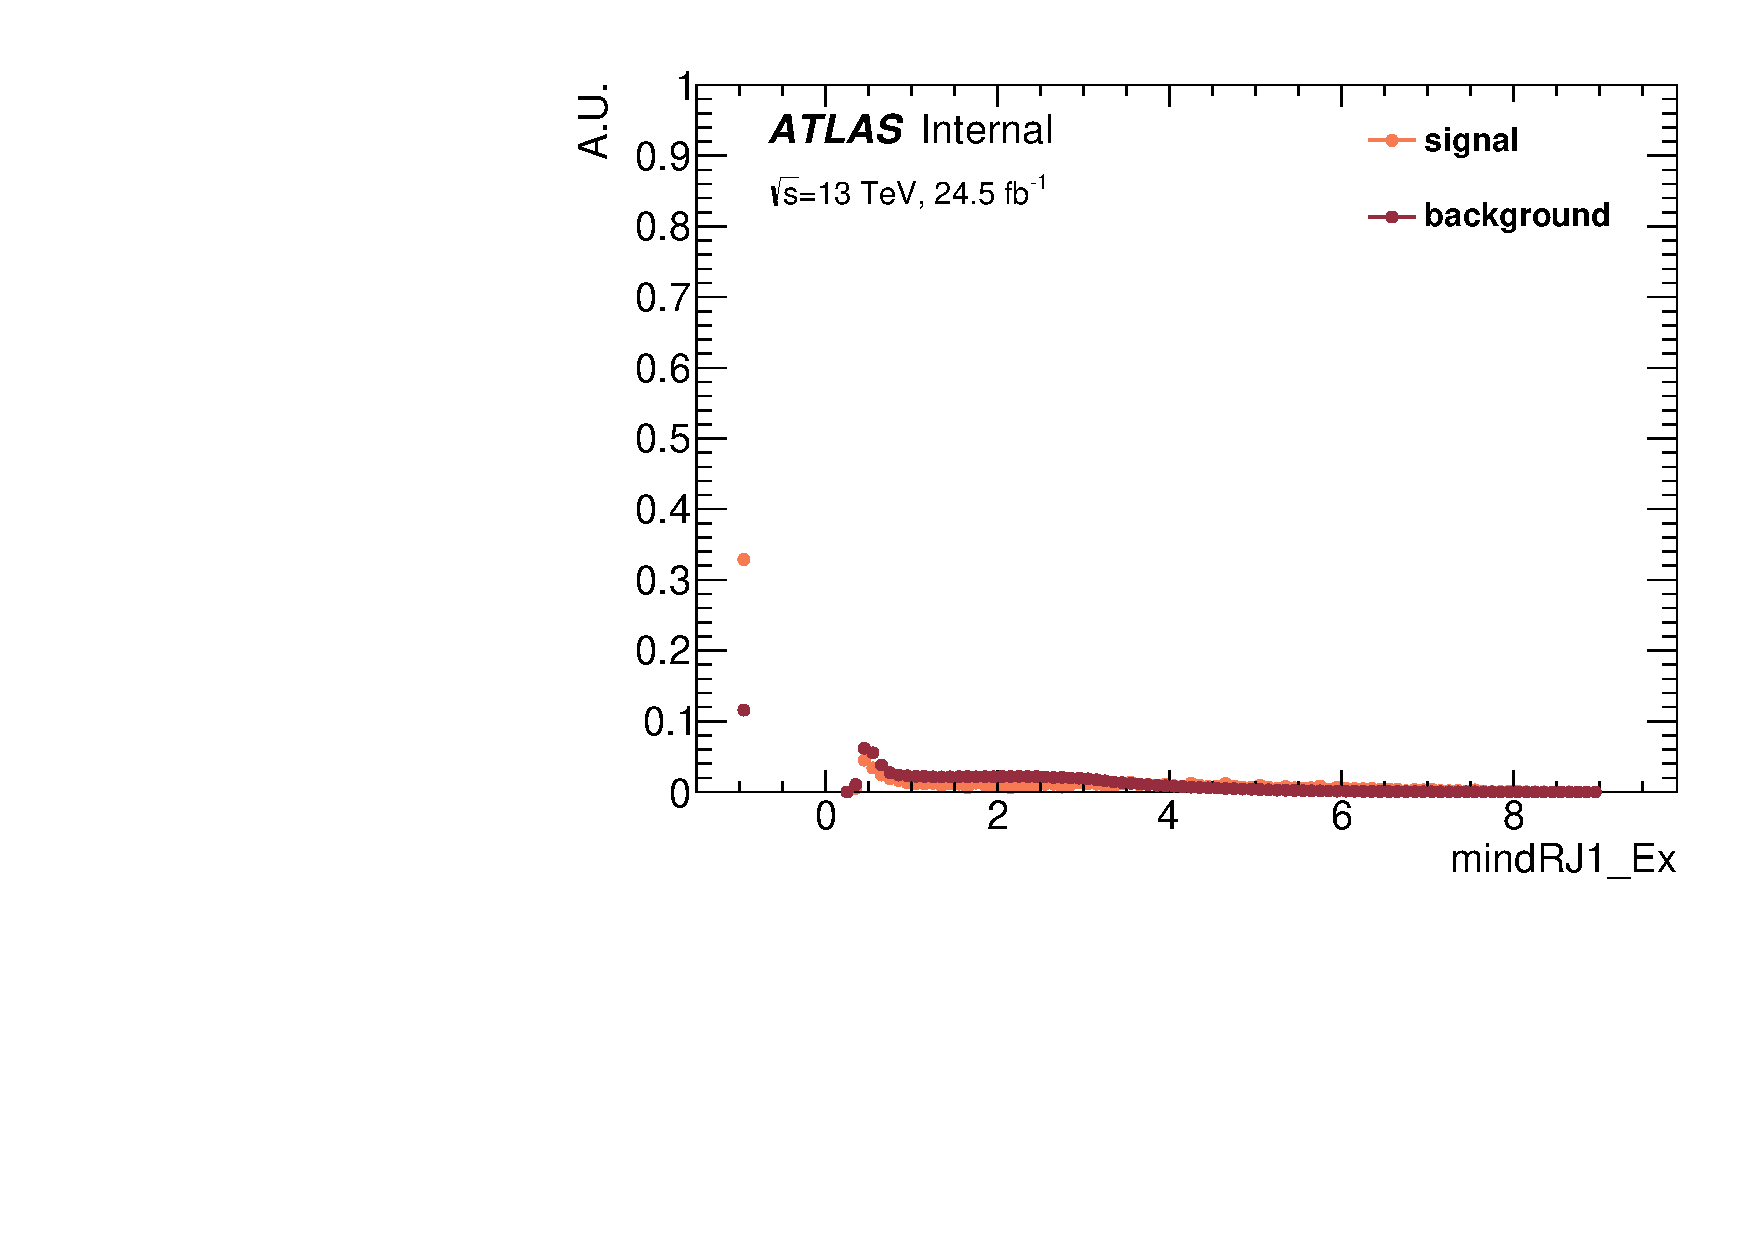
\includegraphics[width=0.3\textwidth]{figures/BDT_mindRJ1_2cen.pdf}
 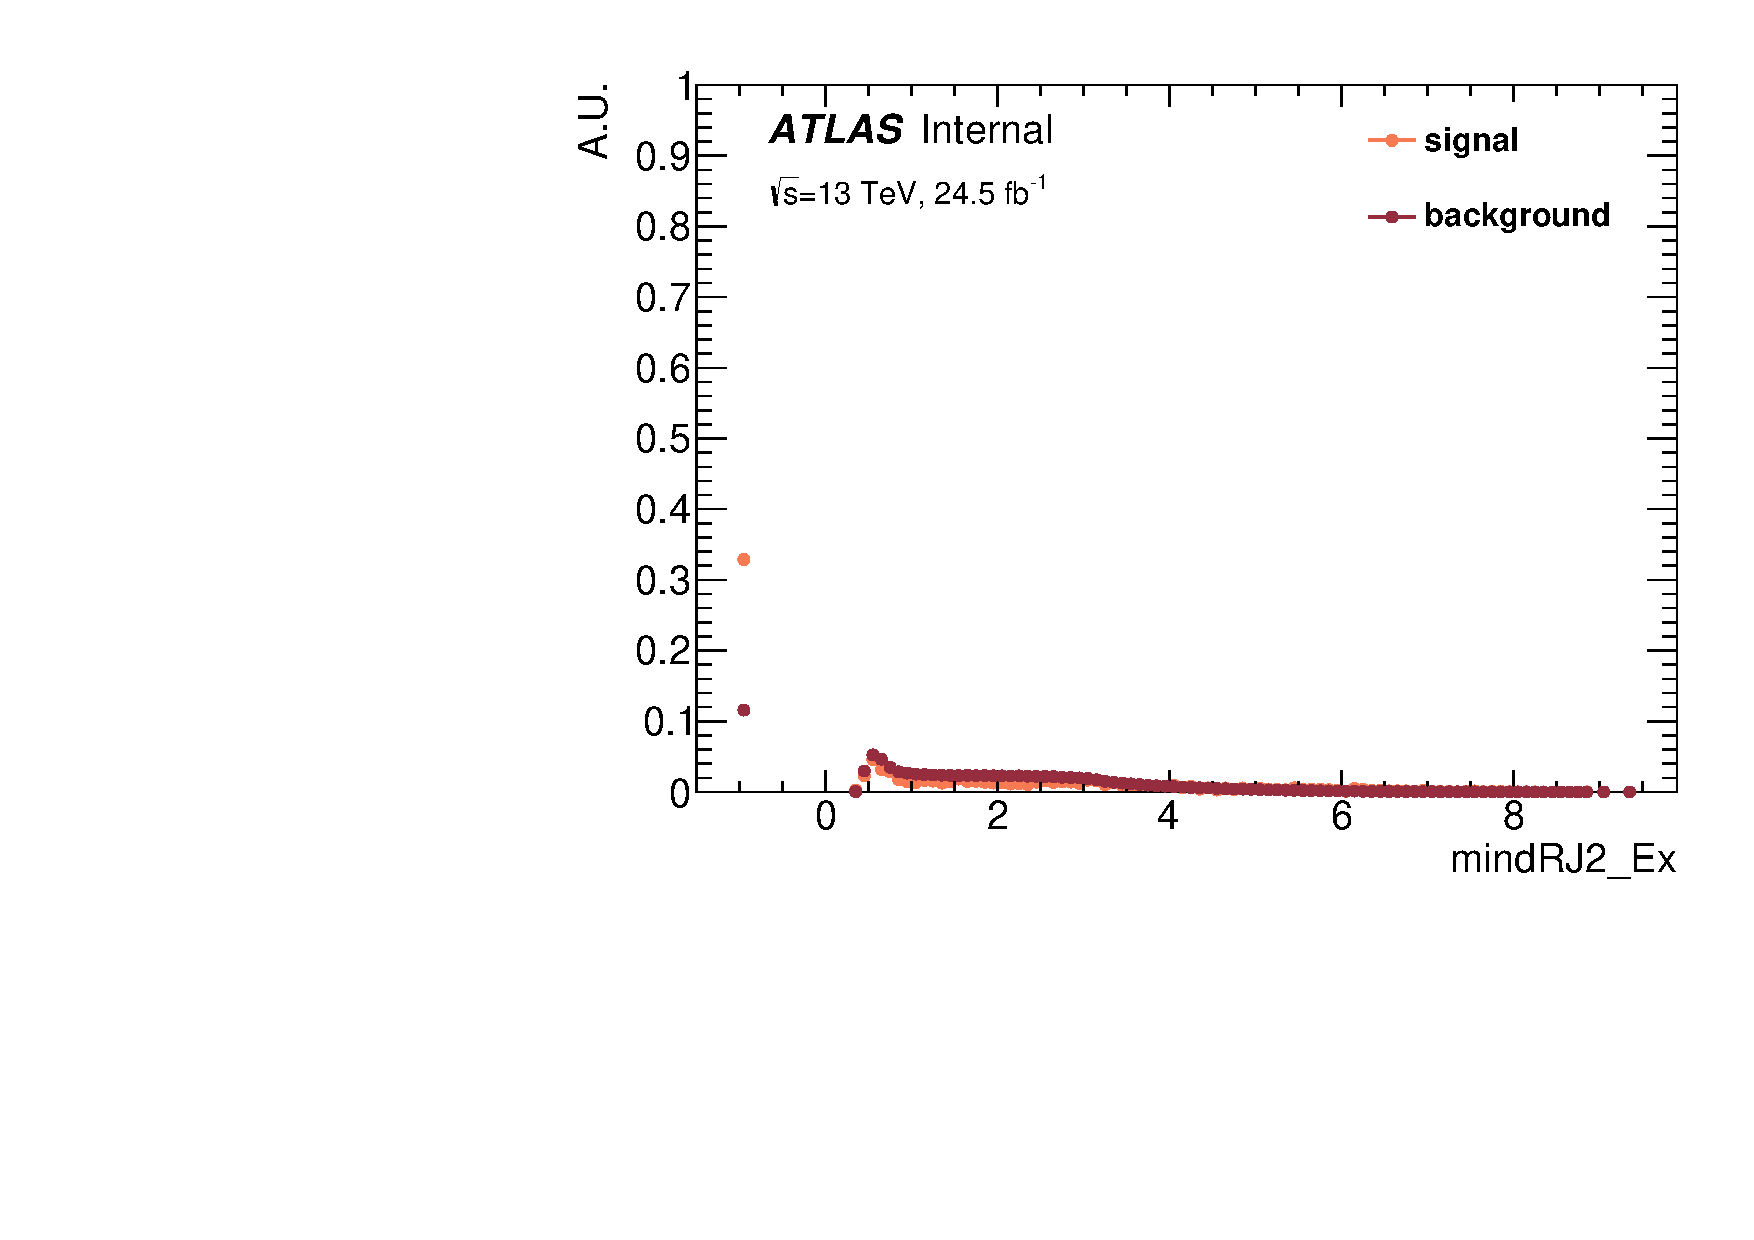
\includegraphics[width=0.3\textwidth]{figures/BDT_mindRJ2_2cen.pdf}
% 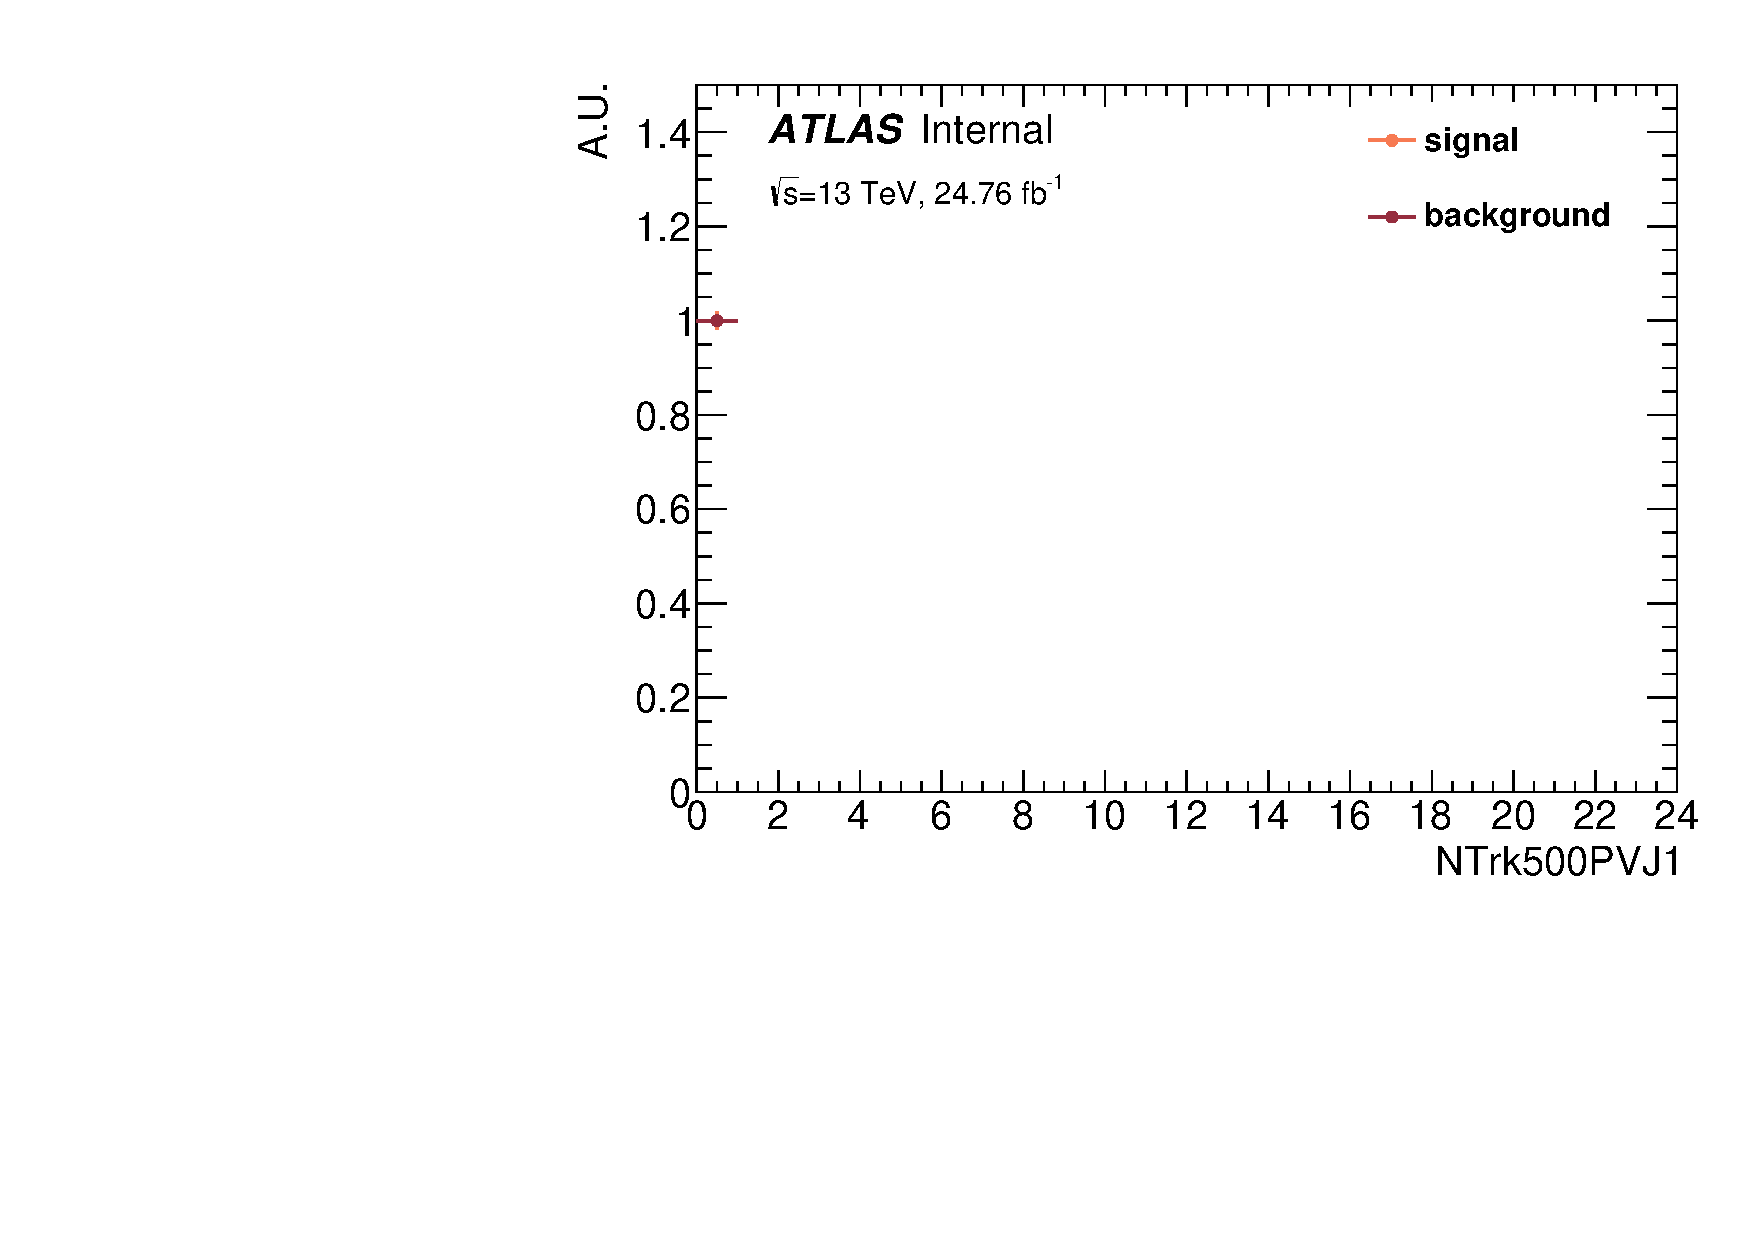
\includegraphics[width=0.3\textwidth]{figures/BDT_NTrk500_J1_2cen.pdf}\\
 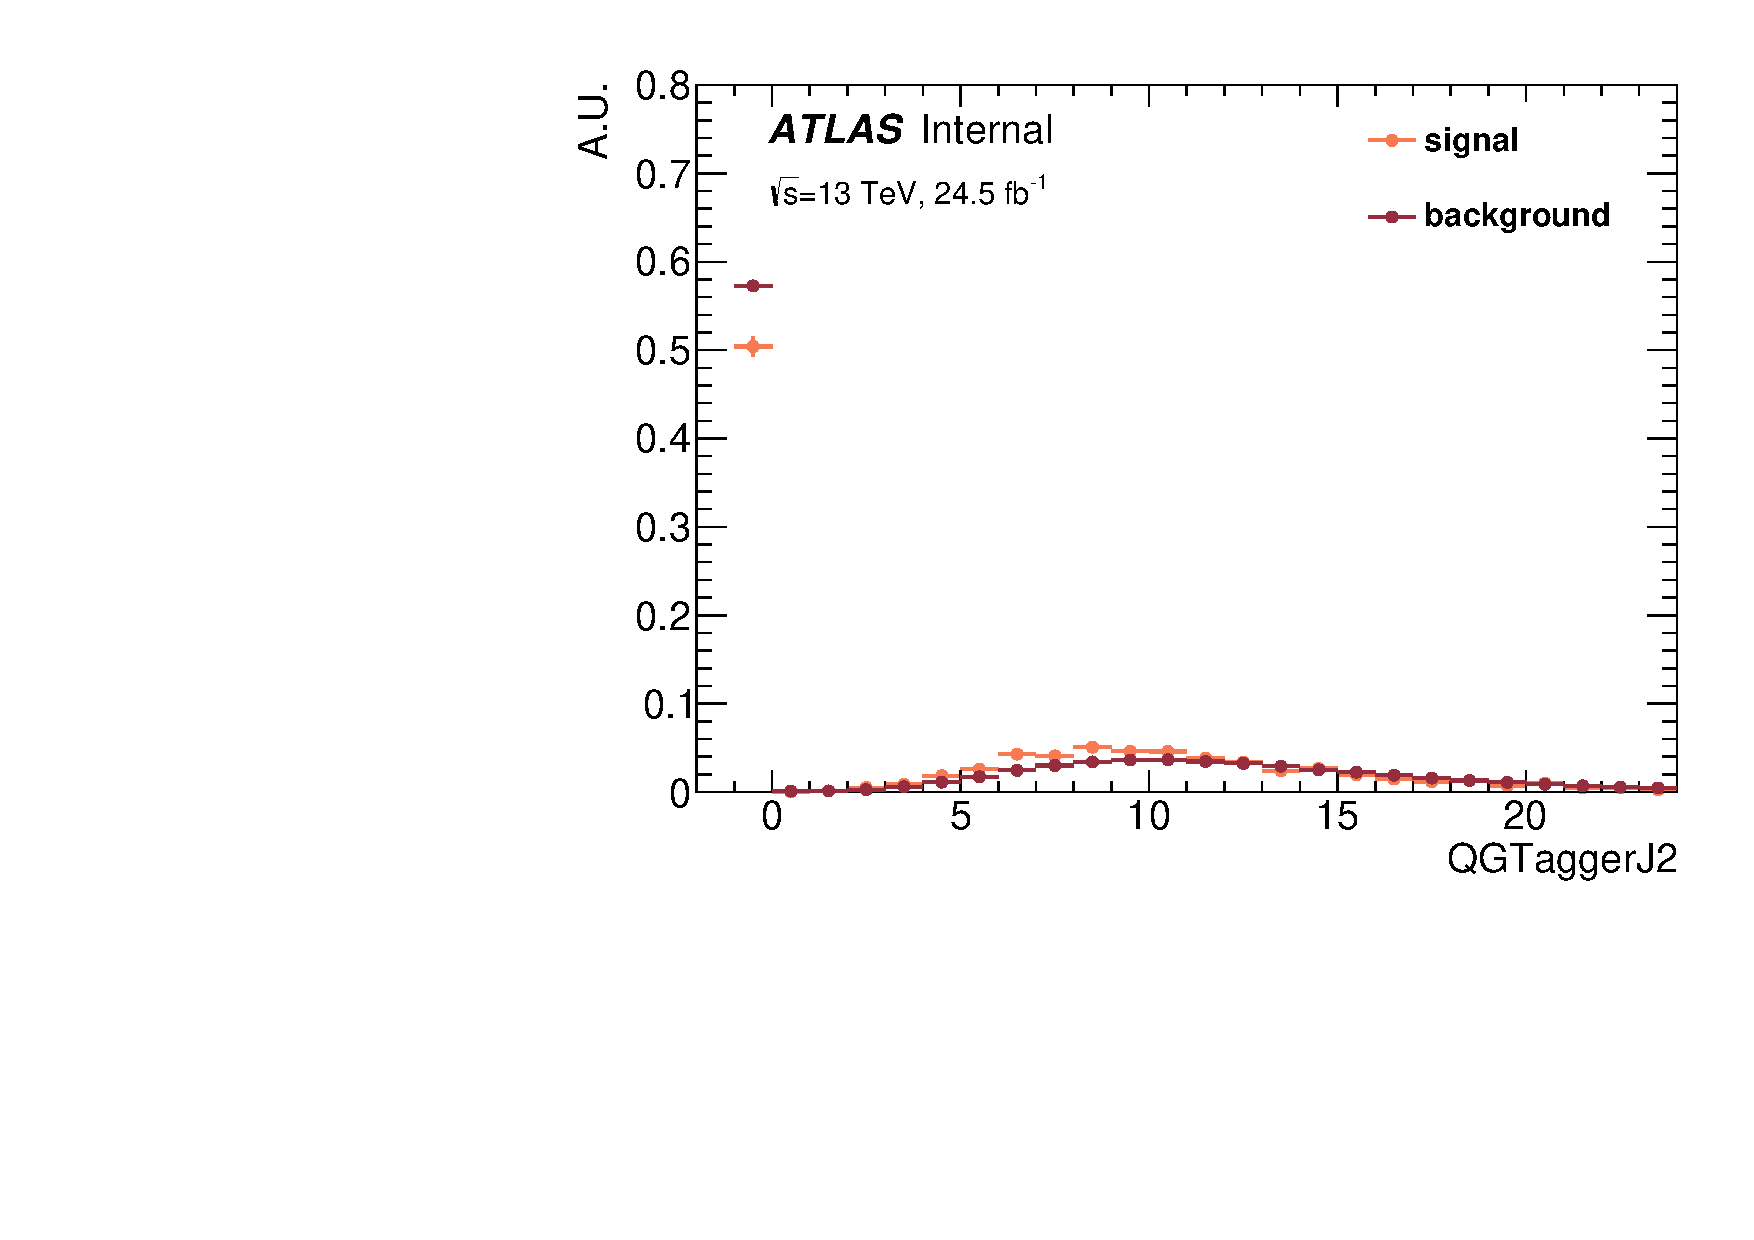
\includegraphics[width=0.3\textwidth]{figures/BDT_NTrk500_J2_2cen.pdf}\\
 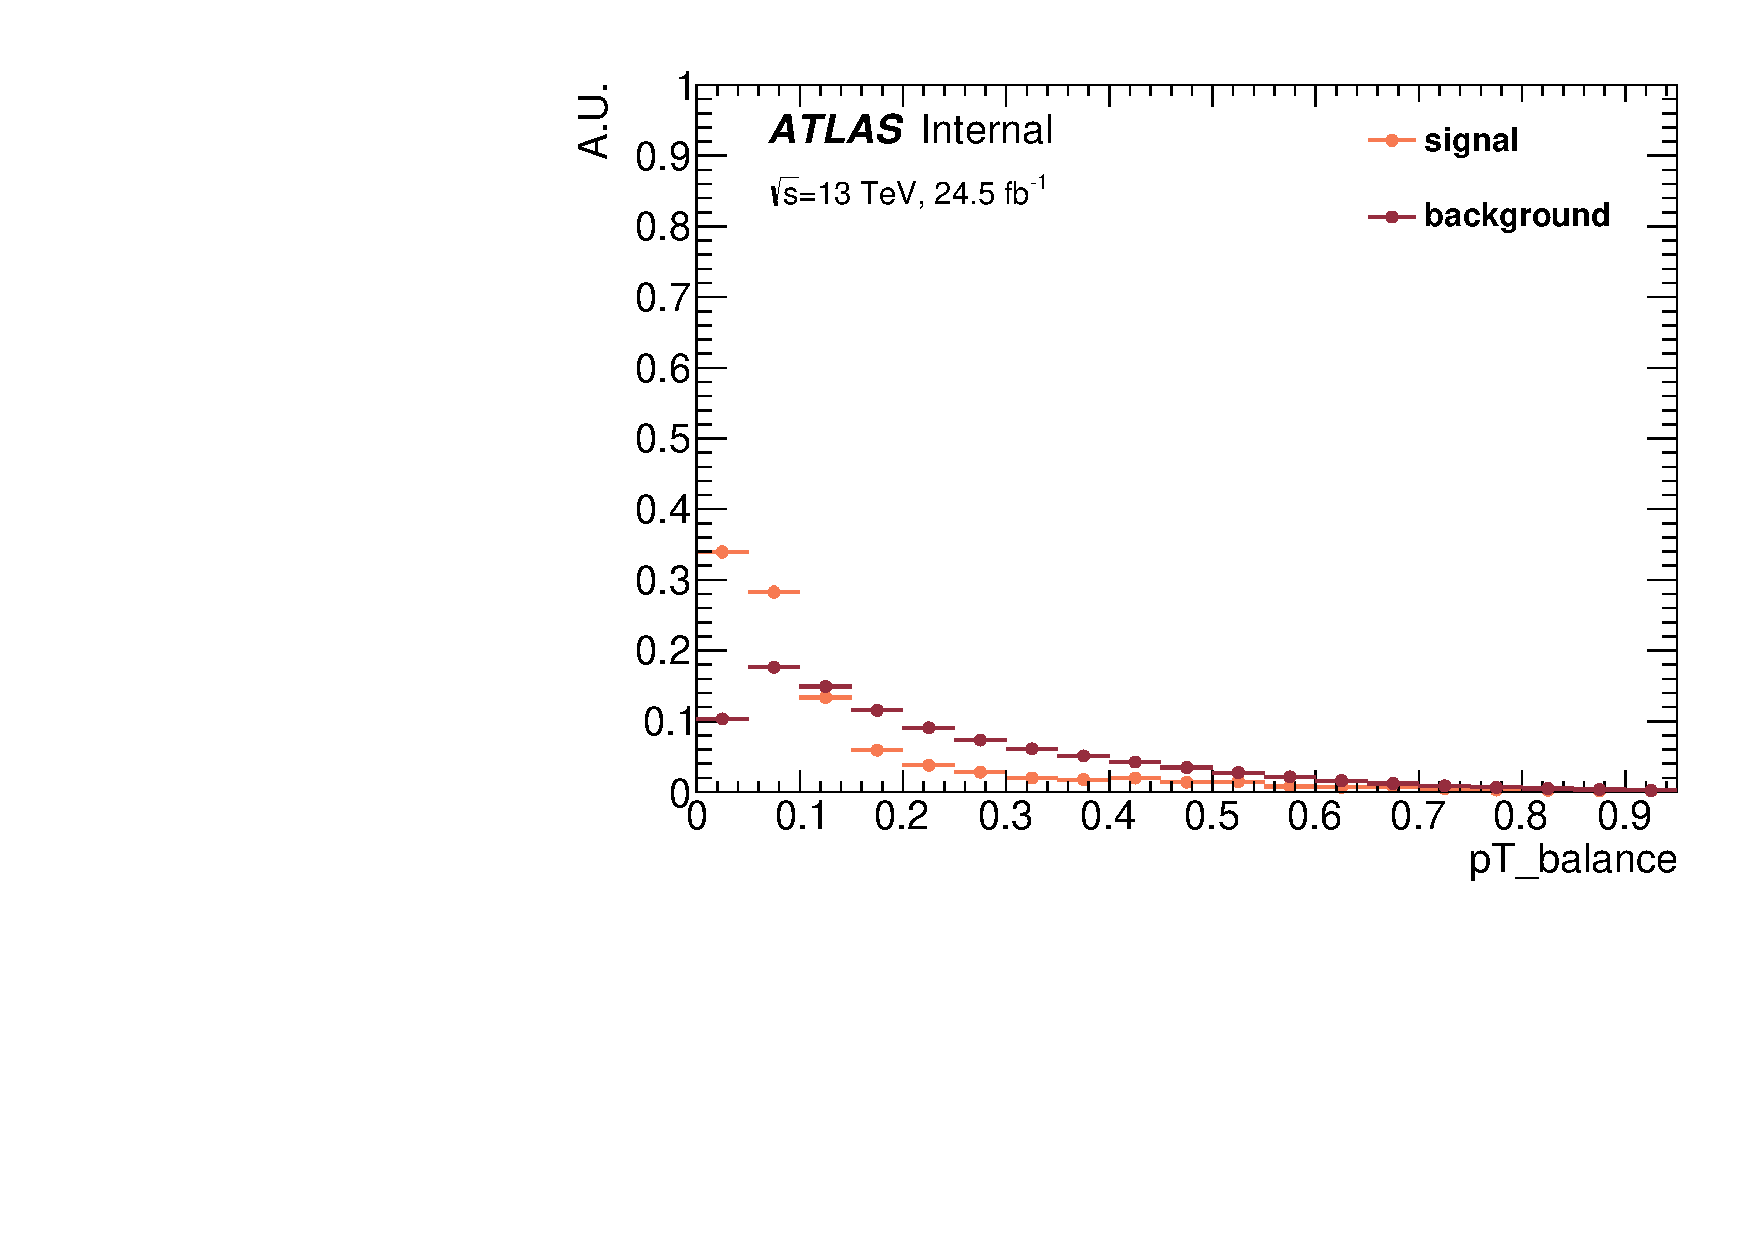
\includegraphics[width=0.3\textwidth]{figures/BDT_pTBalance_2cen.pdf}\\

 %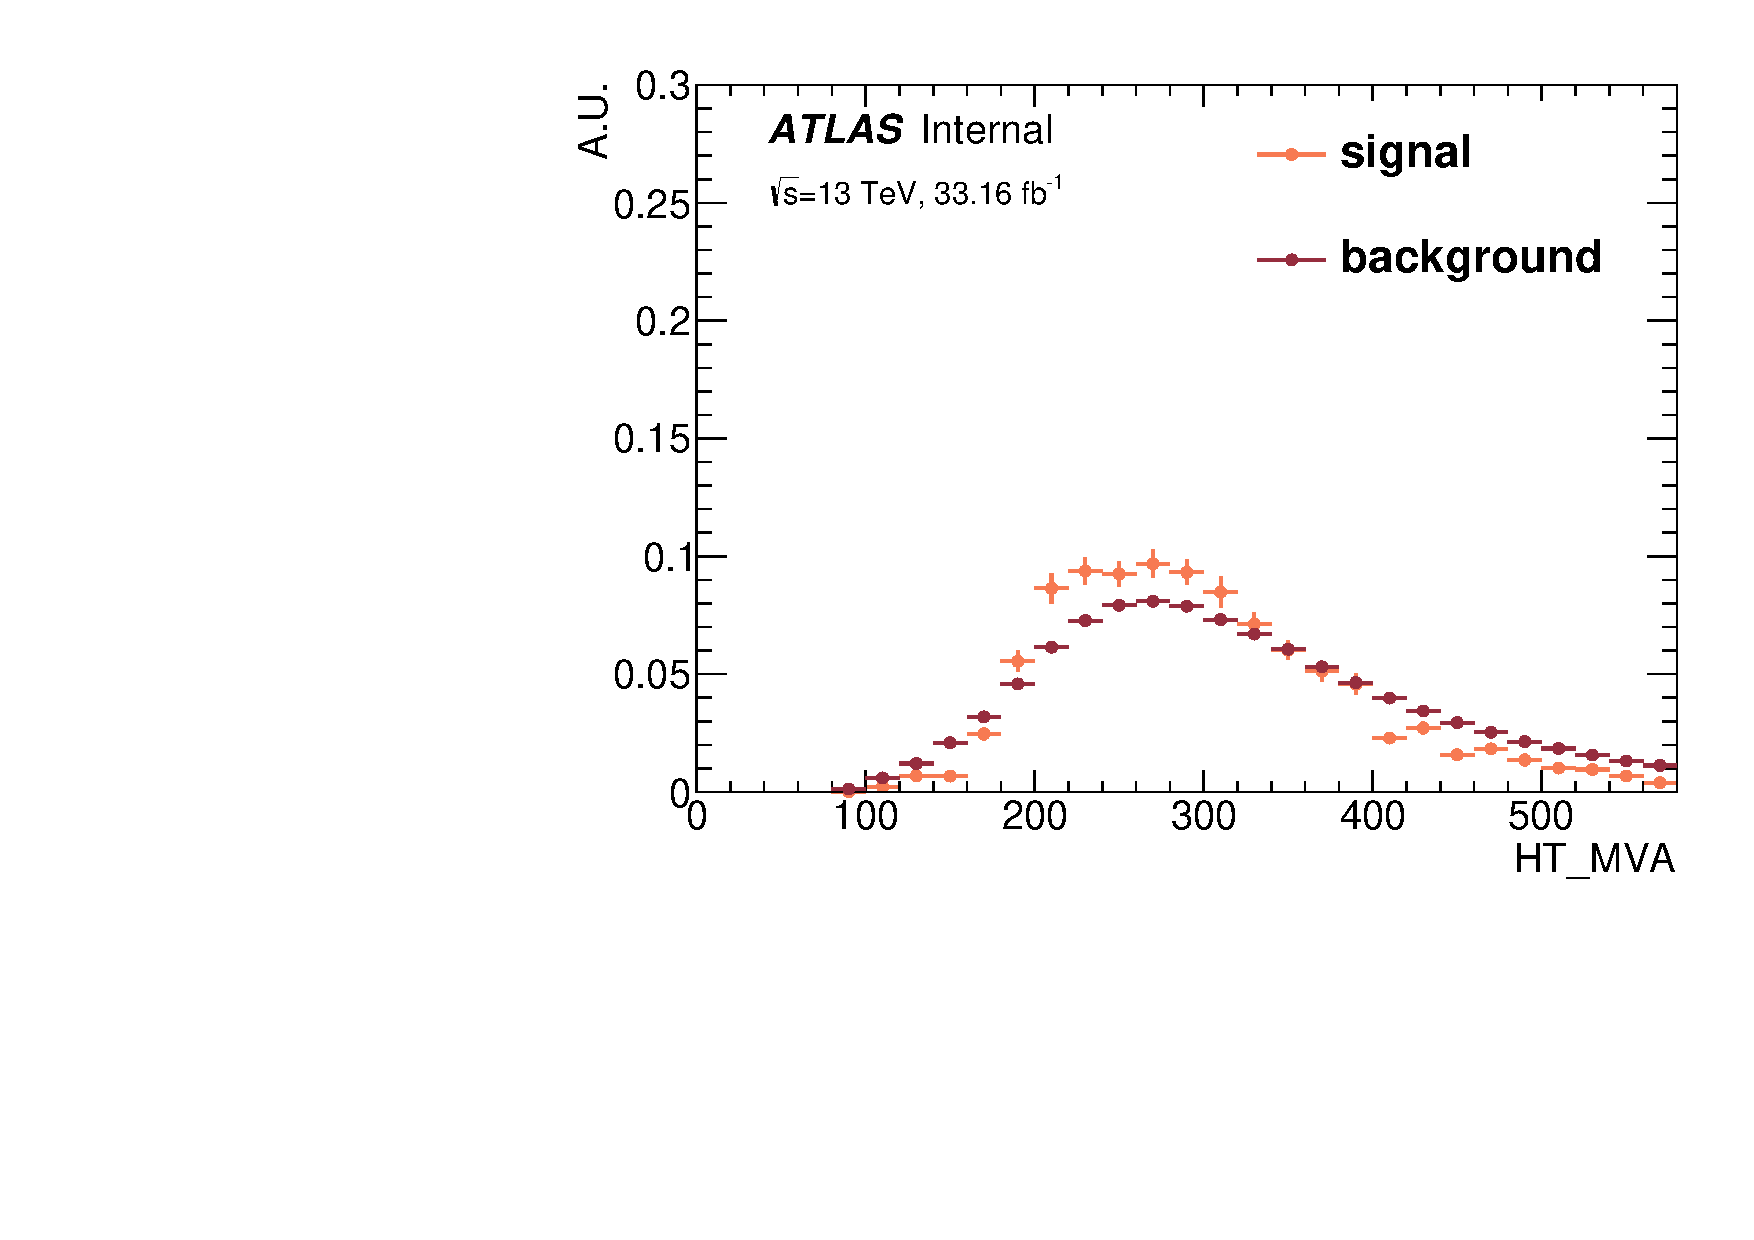
\includegraphics[width=0.3\textwidth]{figures/BDT_HT_2cen.pdf}
\caption{Distributions of BDT input variables of \twocentral channel.  $N_{\rm Trk}($J1$)PV500$ is identically zero because J1 is by definition outside of the tracker acceptance.}
  \label{fig:BDTInputs2cen}
\end{figure}

\begin{figure}[htbp]
  \centering
 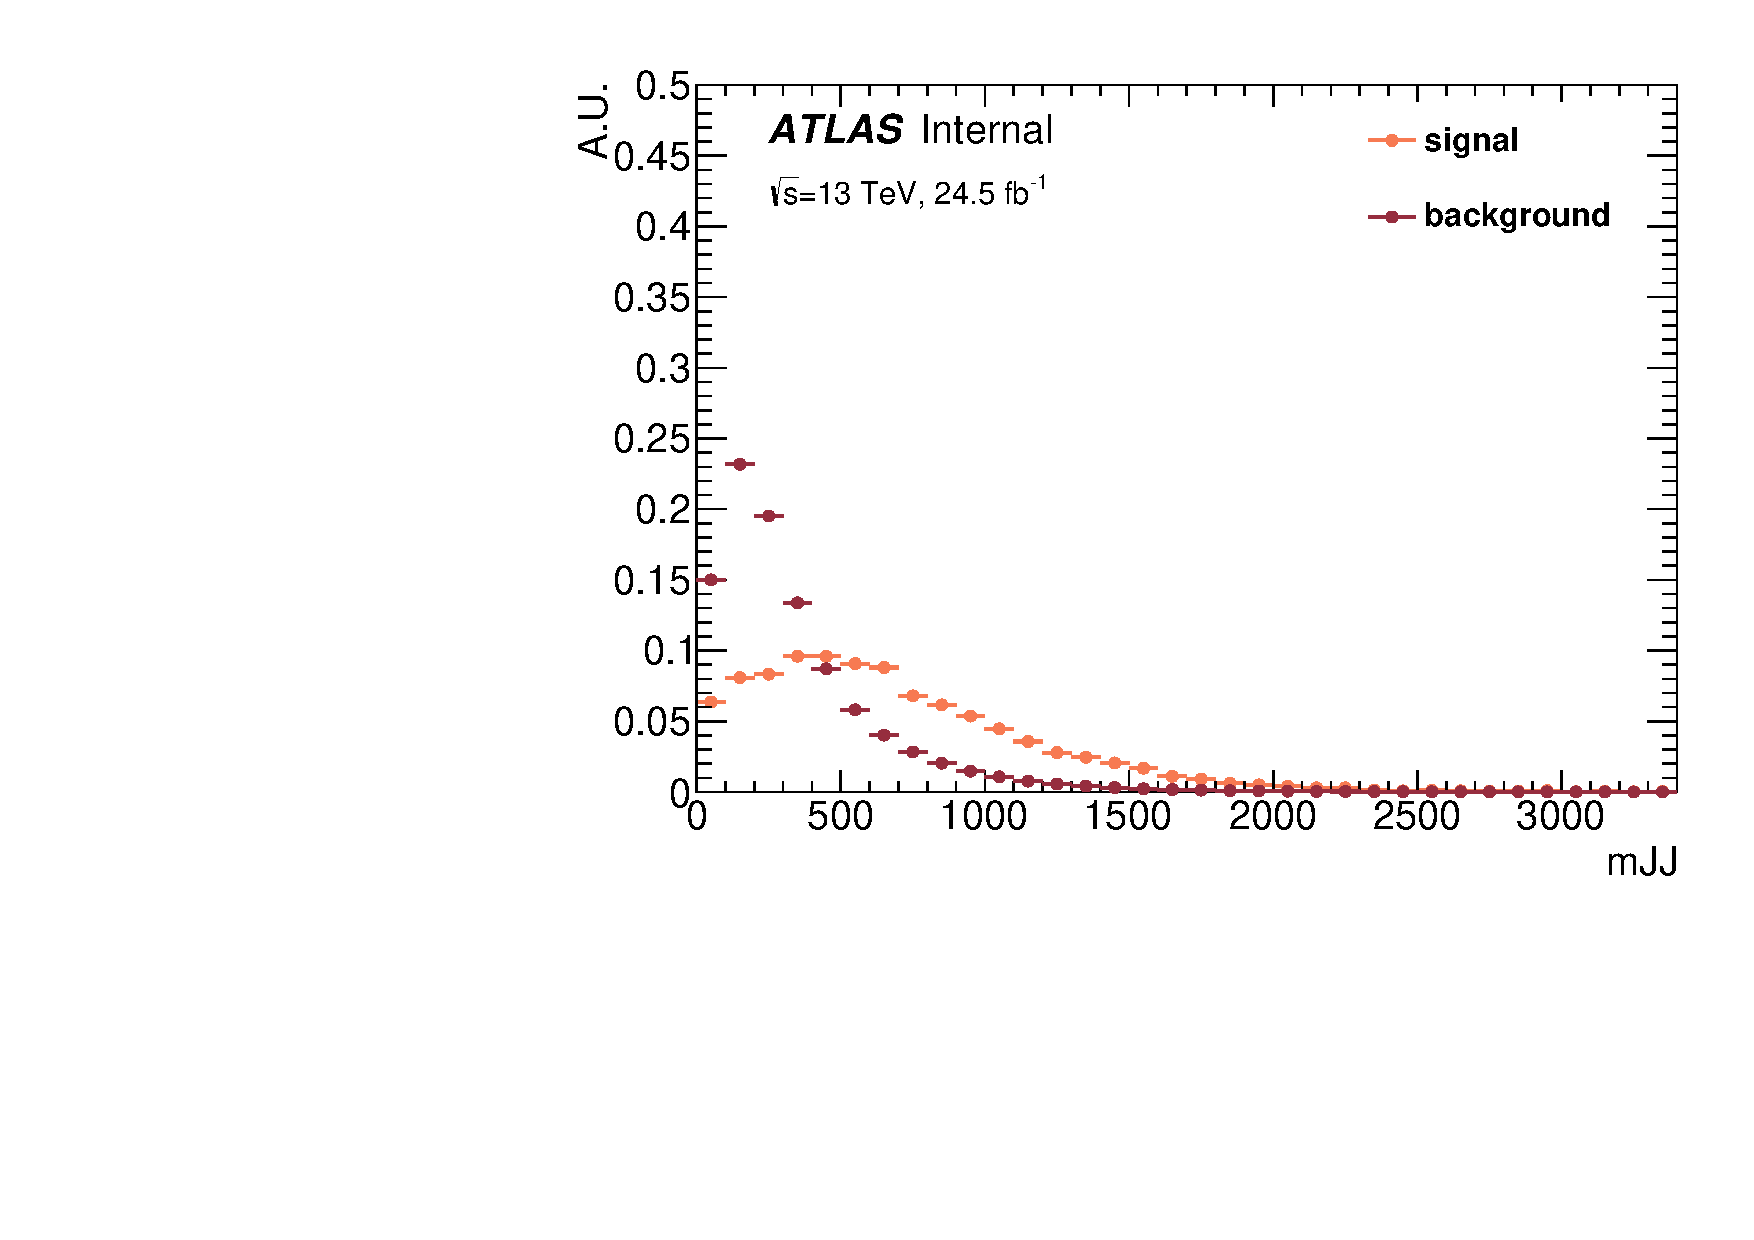
\includegraphics[width=0.3\textwidth]{figures/BDT_mJJ_4cen.pdf}
 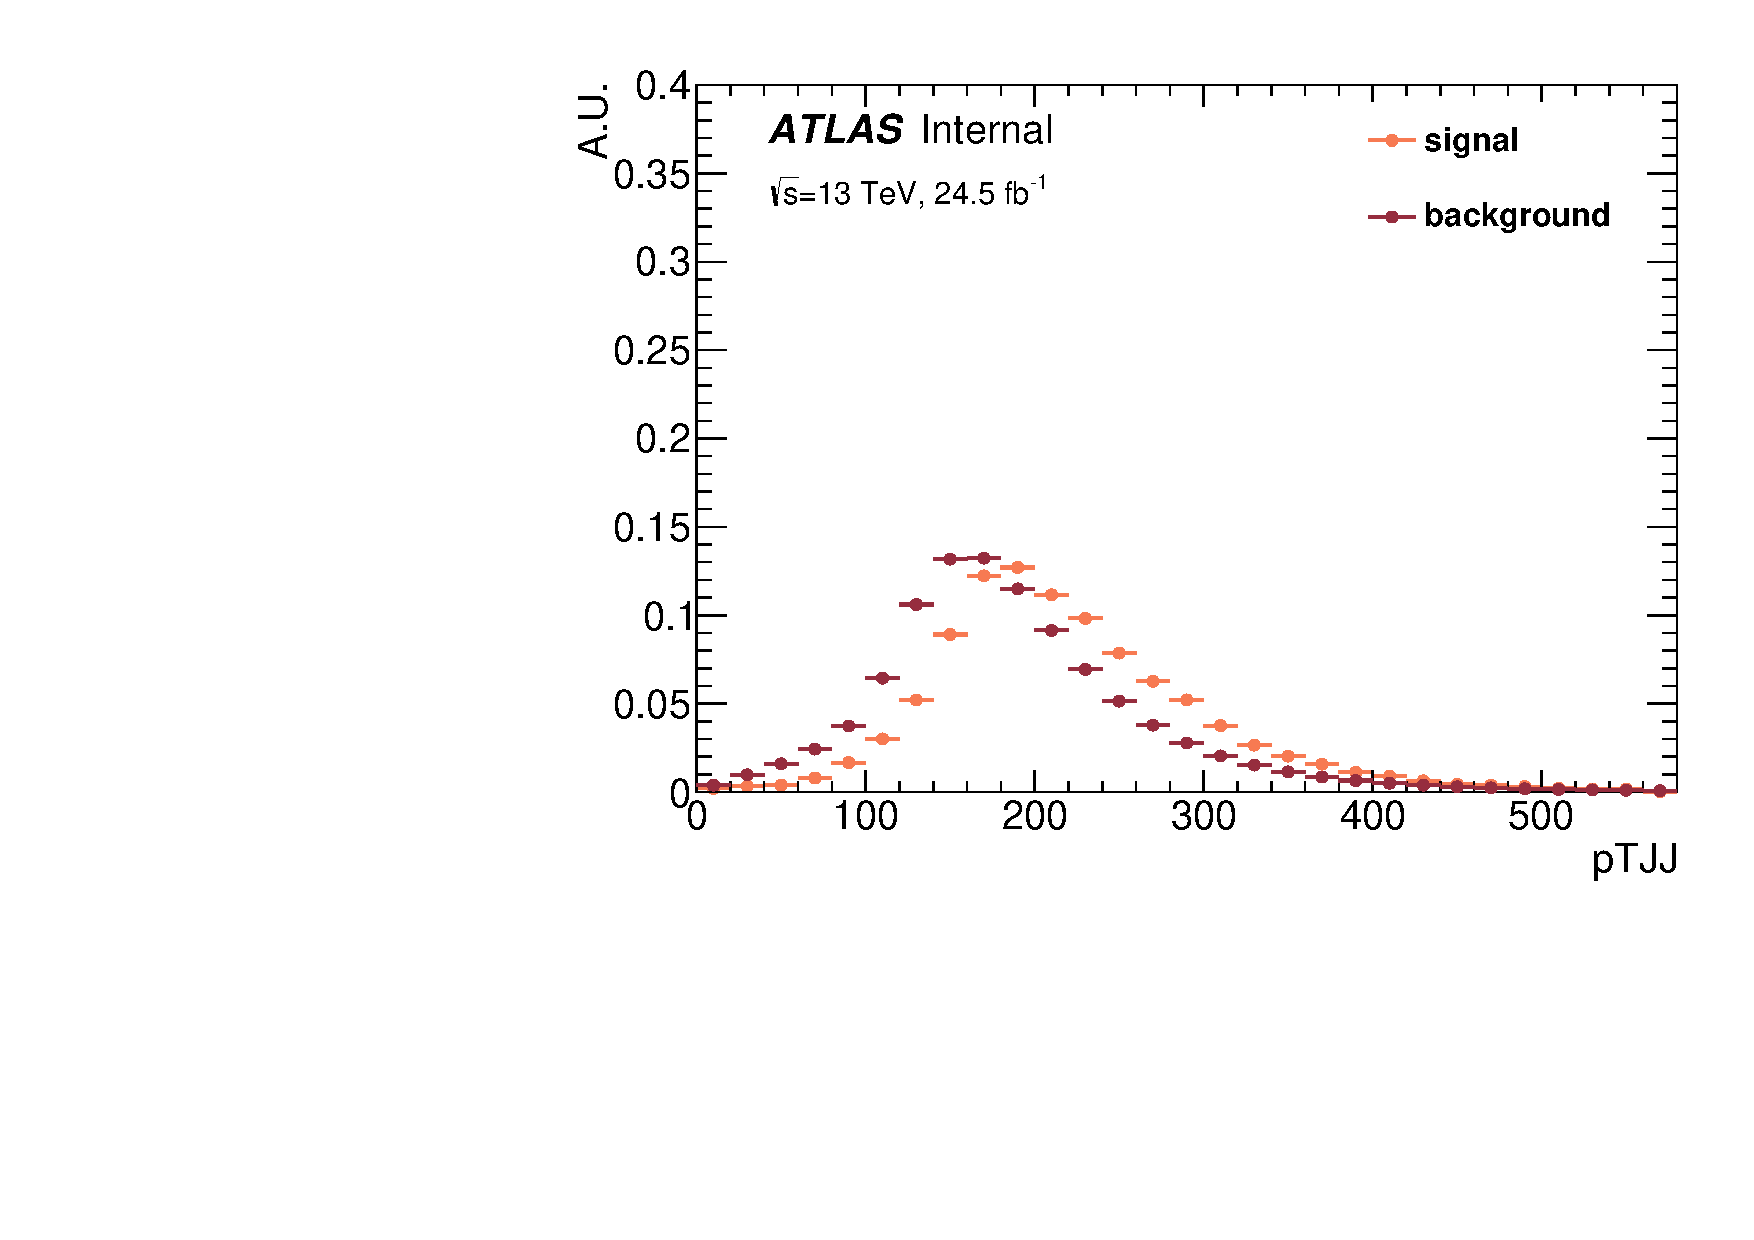
\includegraphics[width=0.3\textwidth]{figures/BDT_pTJJ_4cen.pdf}
 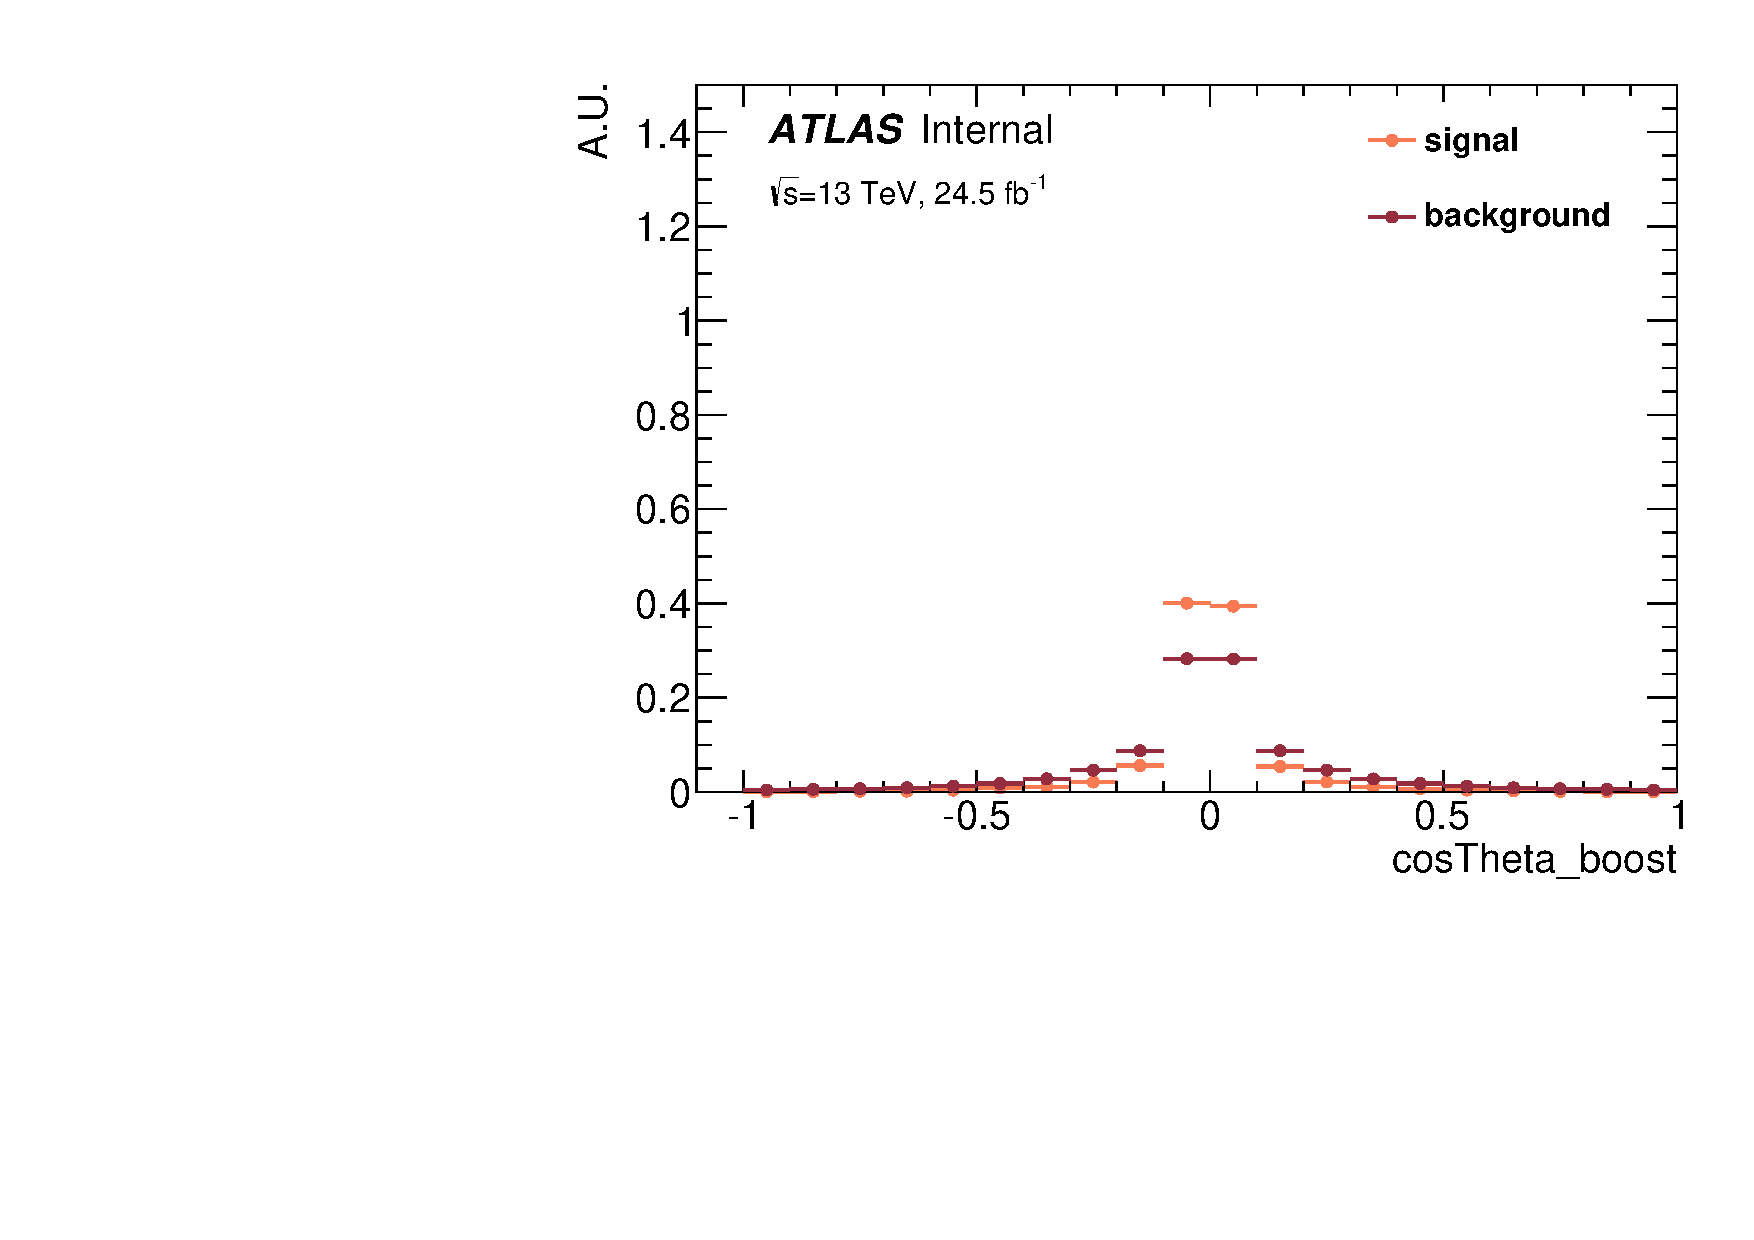
\includegraphics[width=0.3\textwidth]{figures/BDT_cosTheta_4cen.pdf}\\
 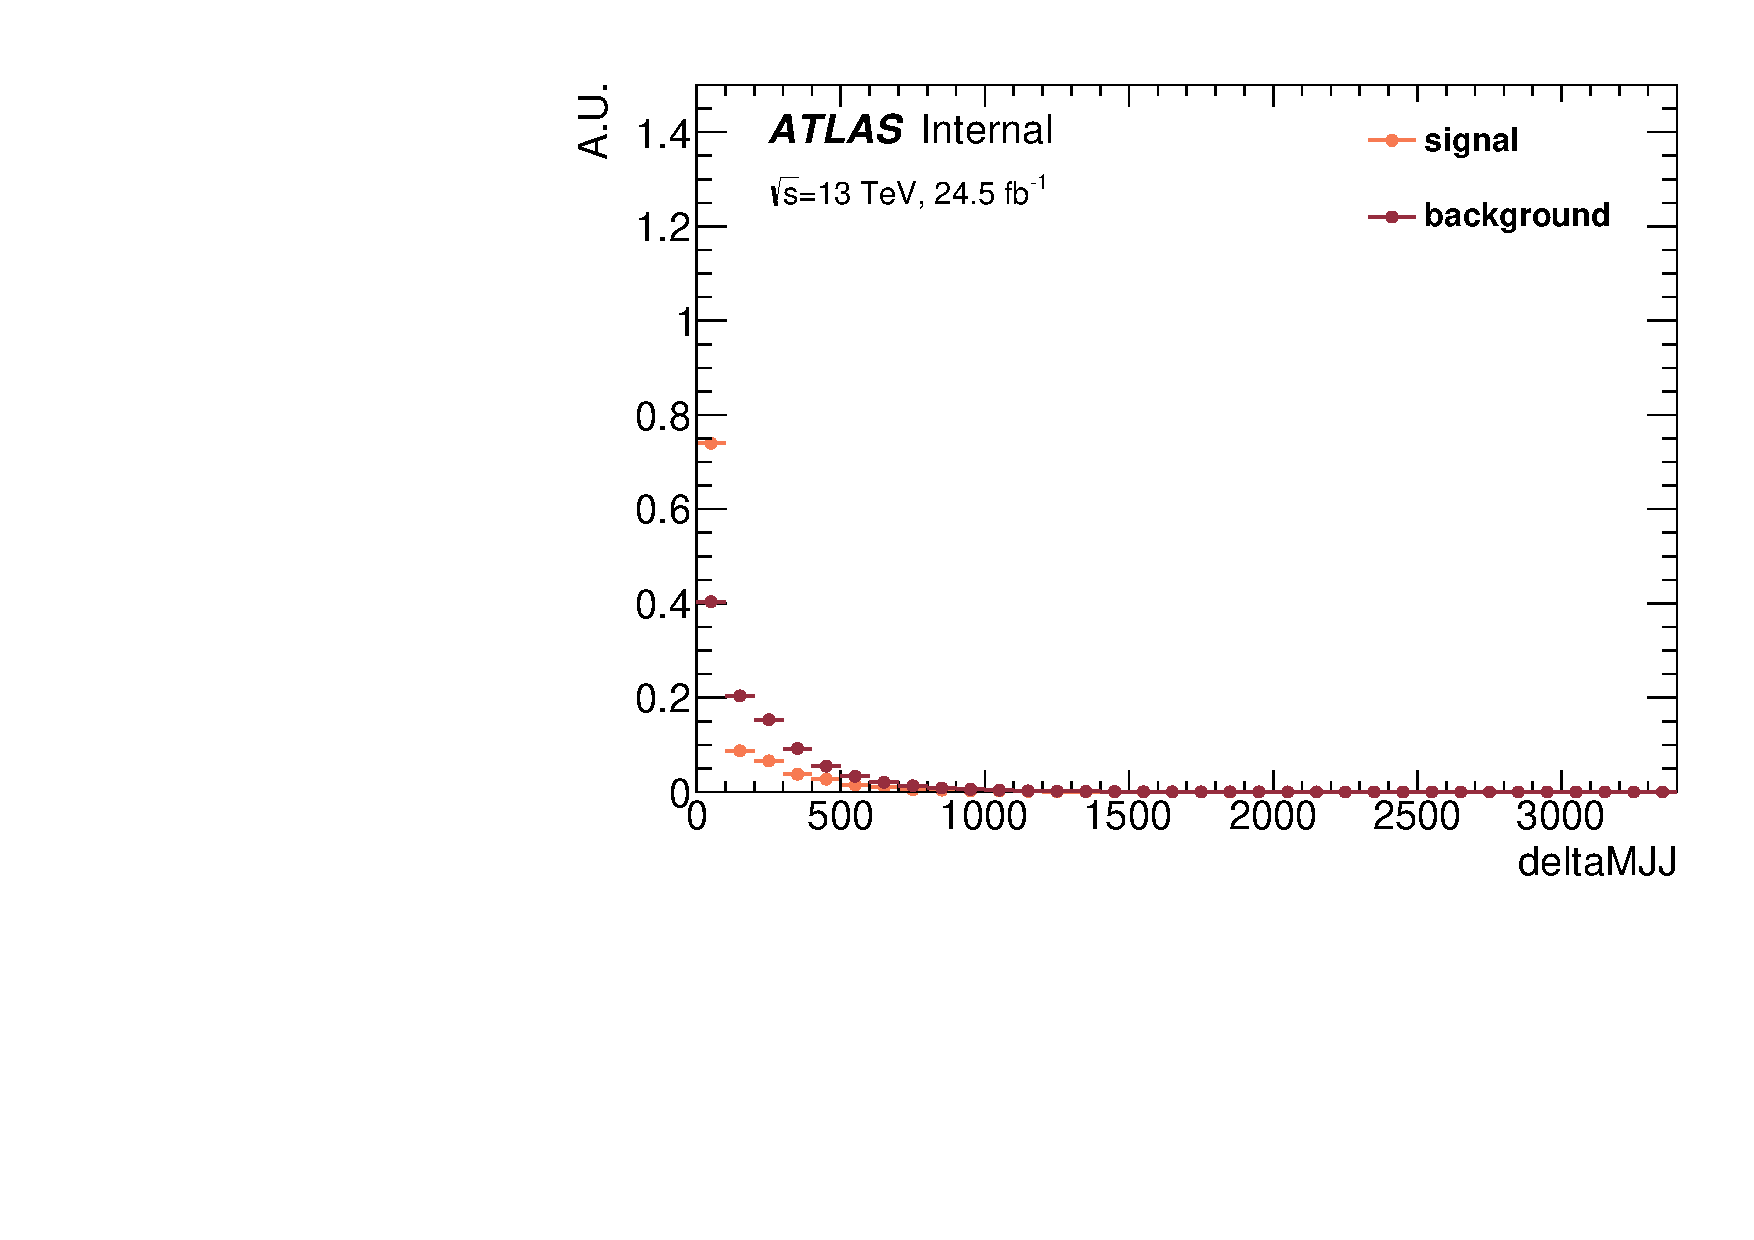
\includegraphics[width=0.3\textwidth]{figures/BDT_deltaMJJ_4cen.pdf}
 % 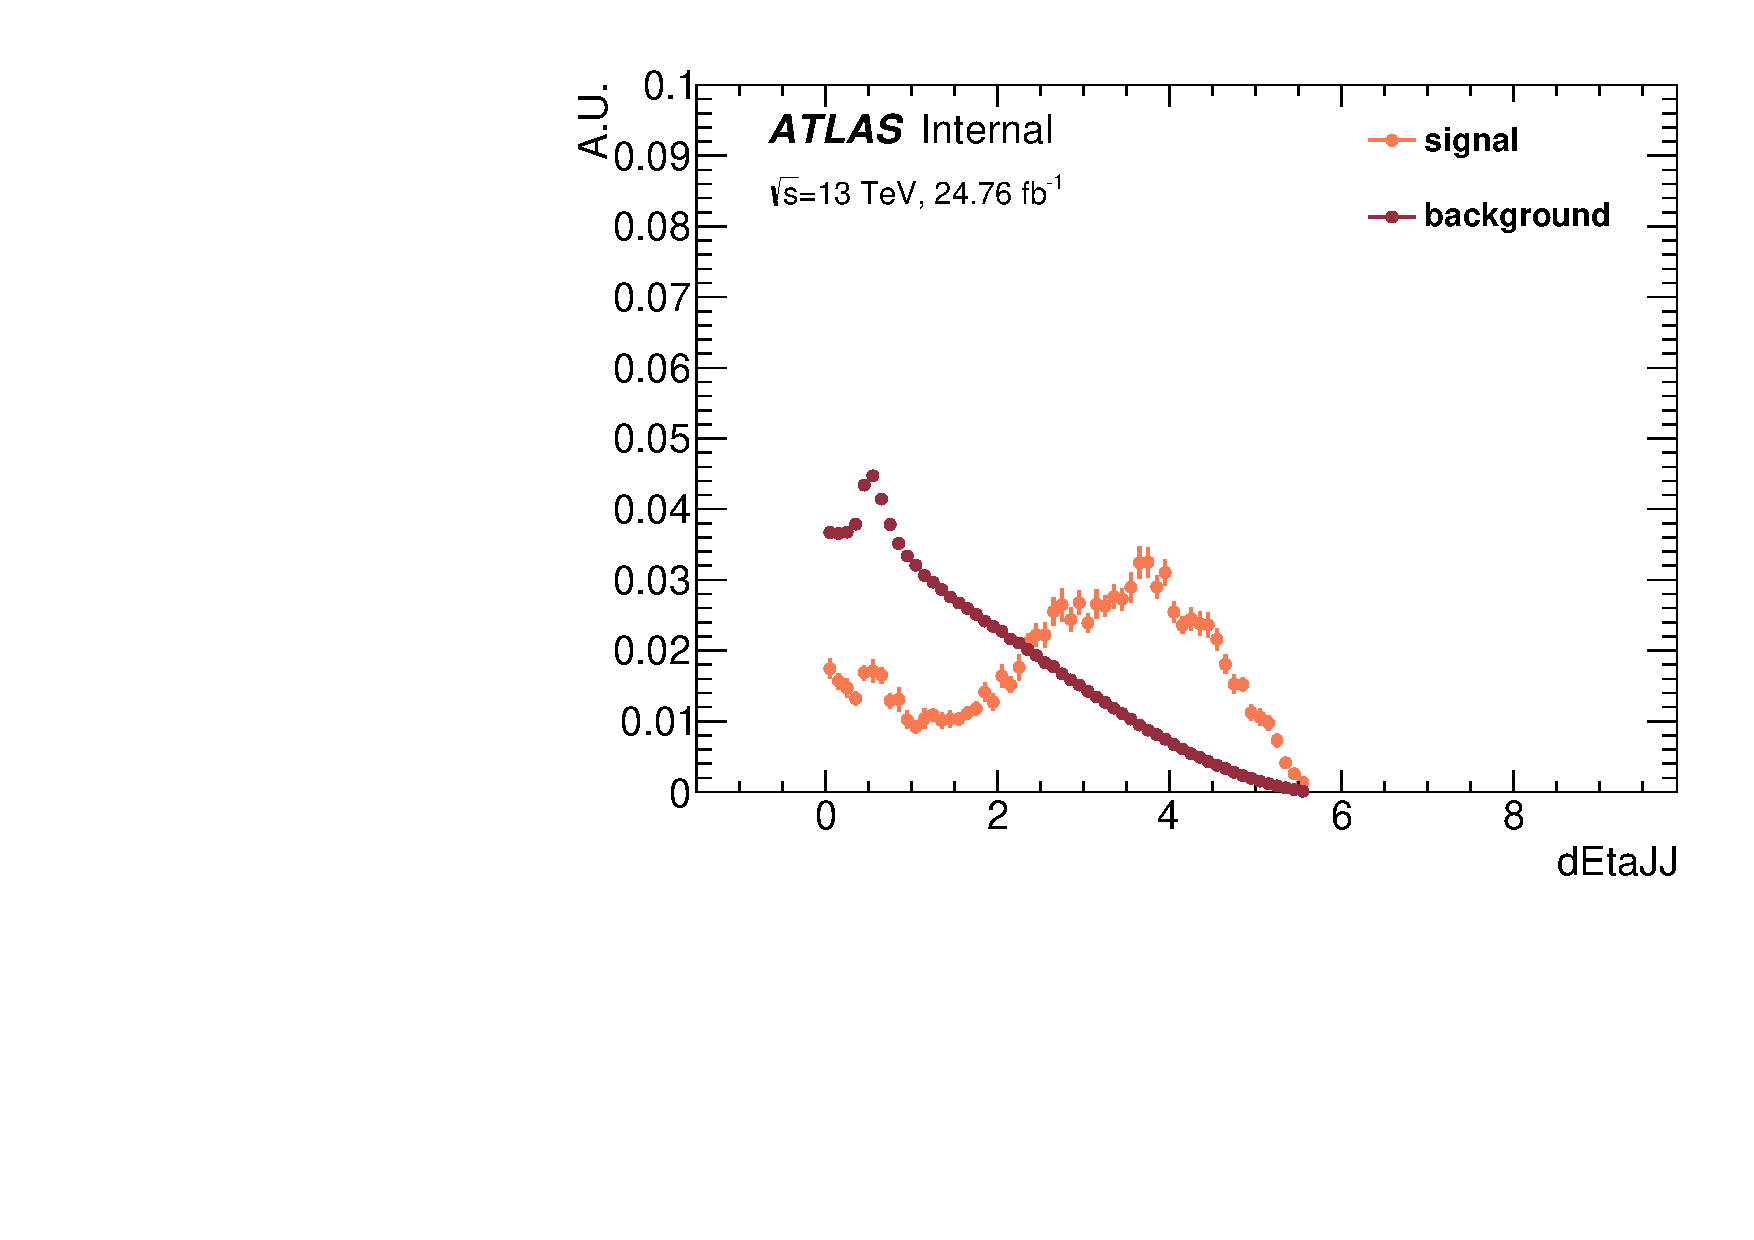
\includegraphics[width=0.3\textwidth]{figures/BDT_dEtaJJ_4cen.pdf}
 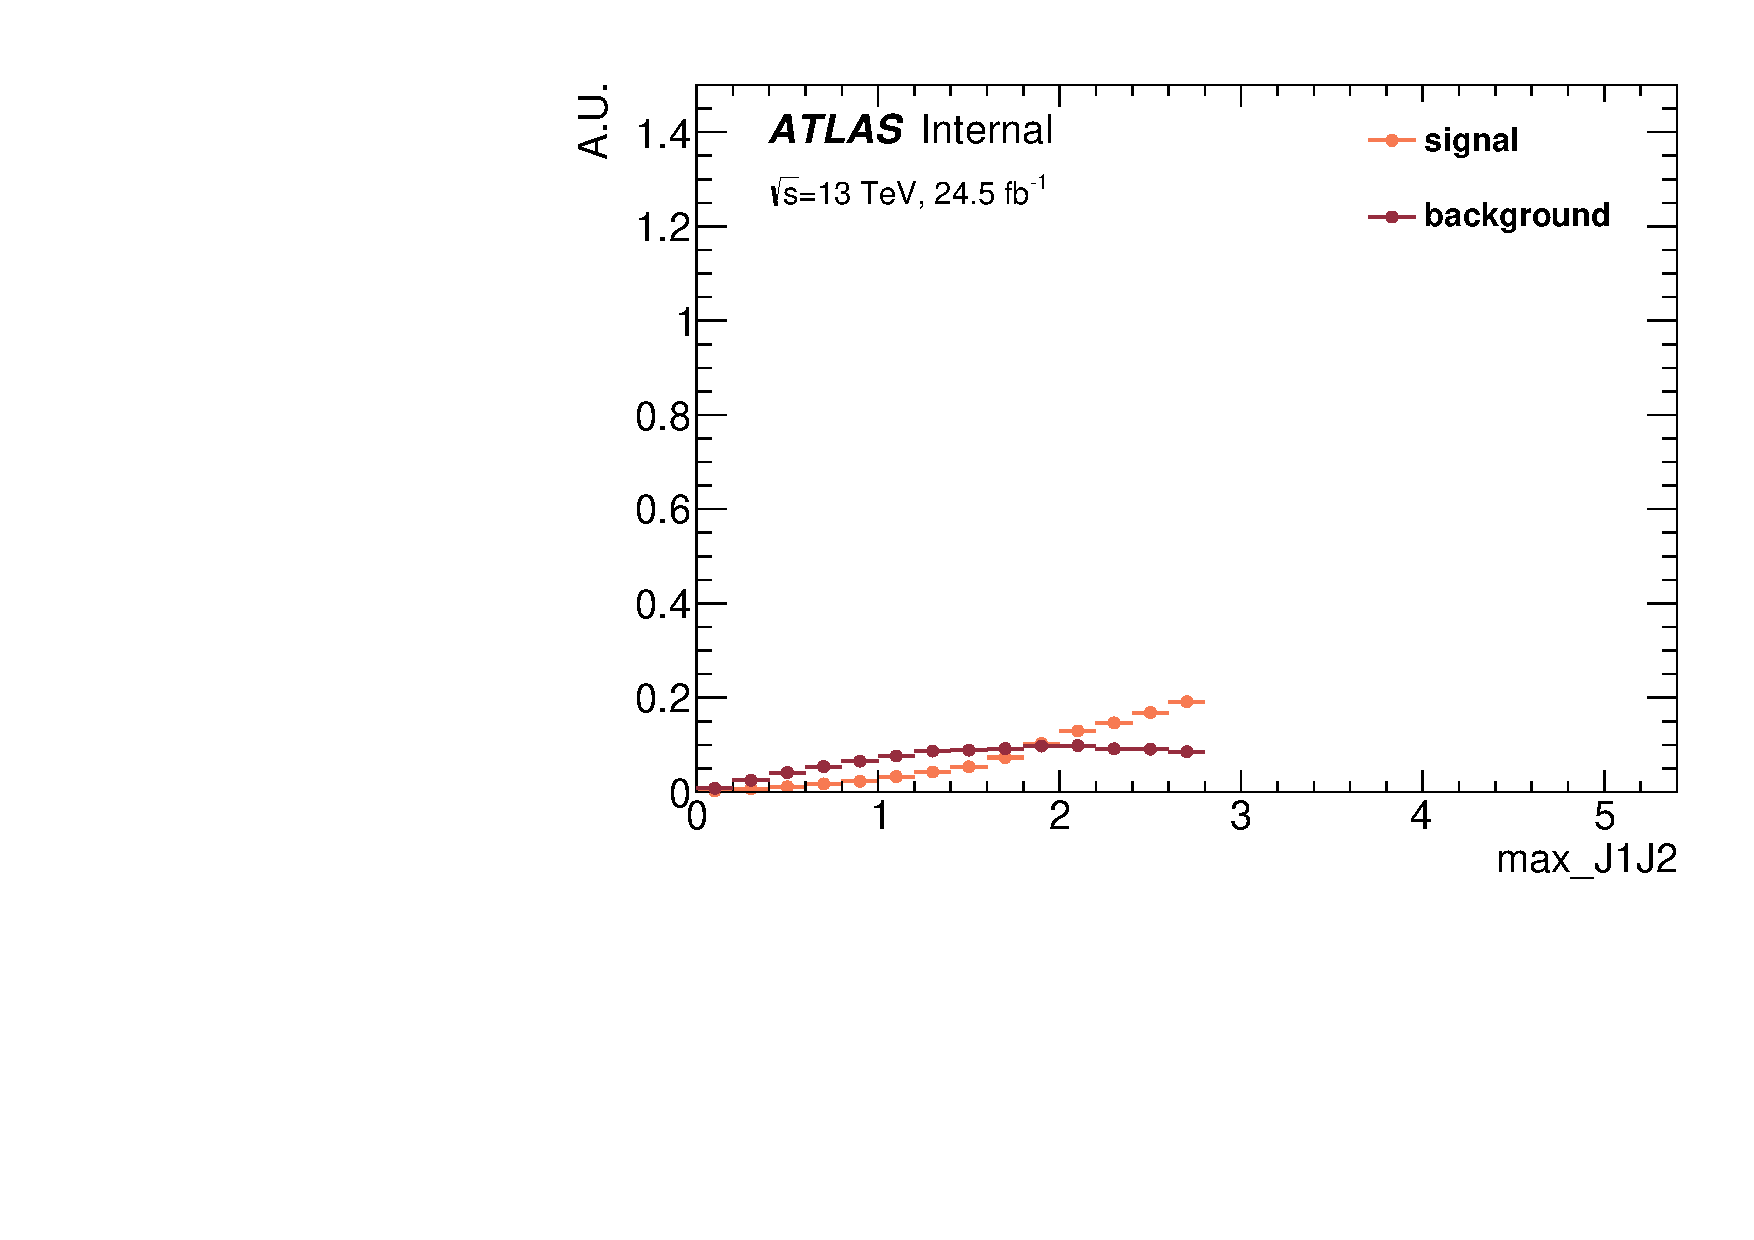
\includegraphics[width=0.3\textwidth]{figures/BDT_maxJ1J2_4cen.pdf}
 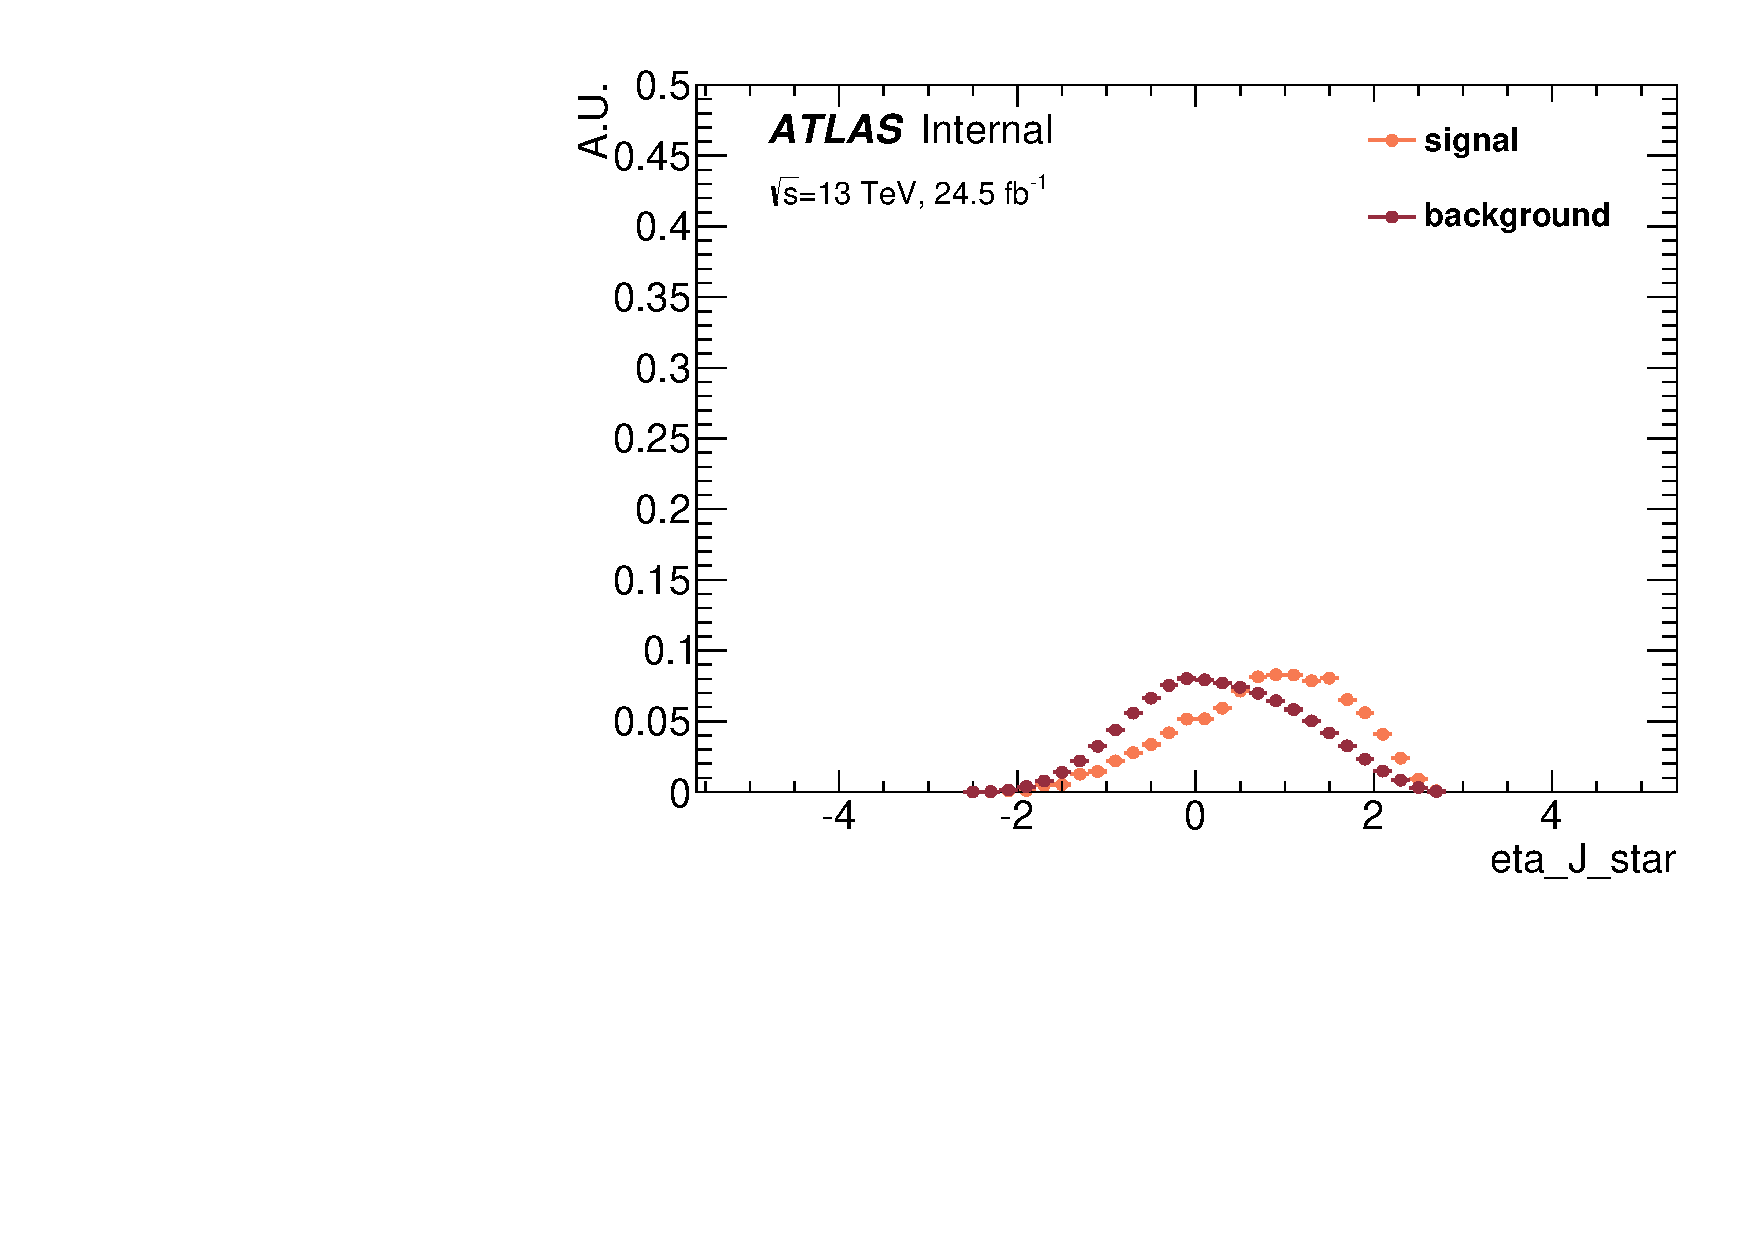
\includegraphics[width=0.3\textwidth]{figures/BDT_etaJstar_4cen.pdf}\\
 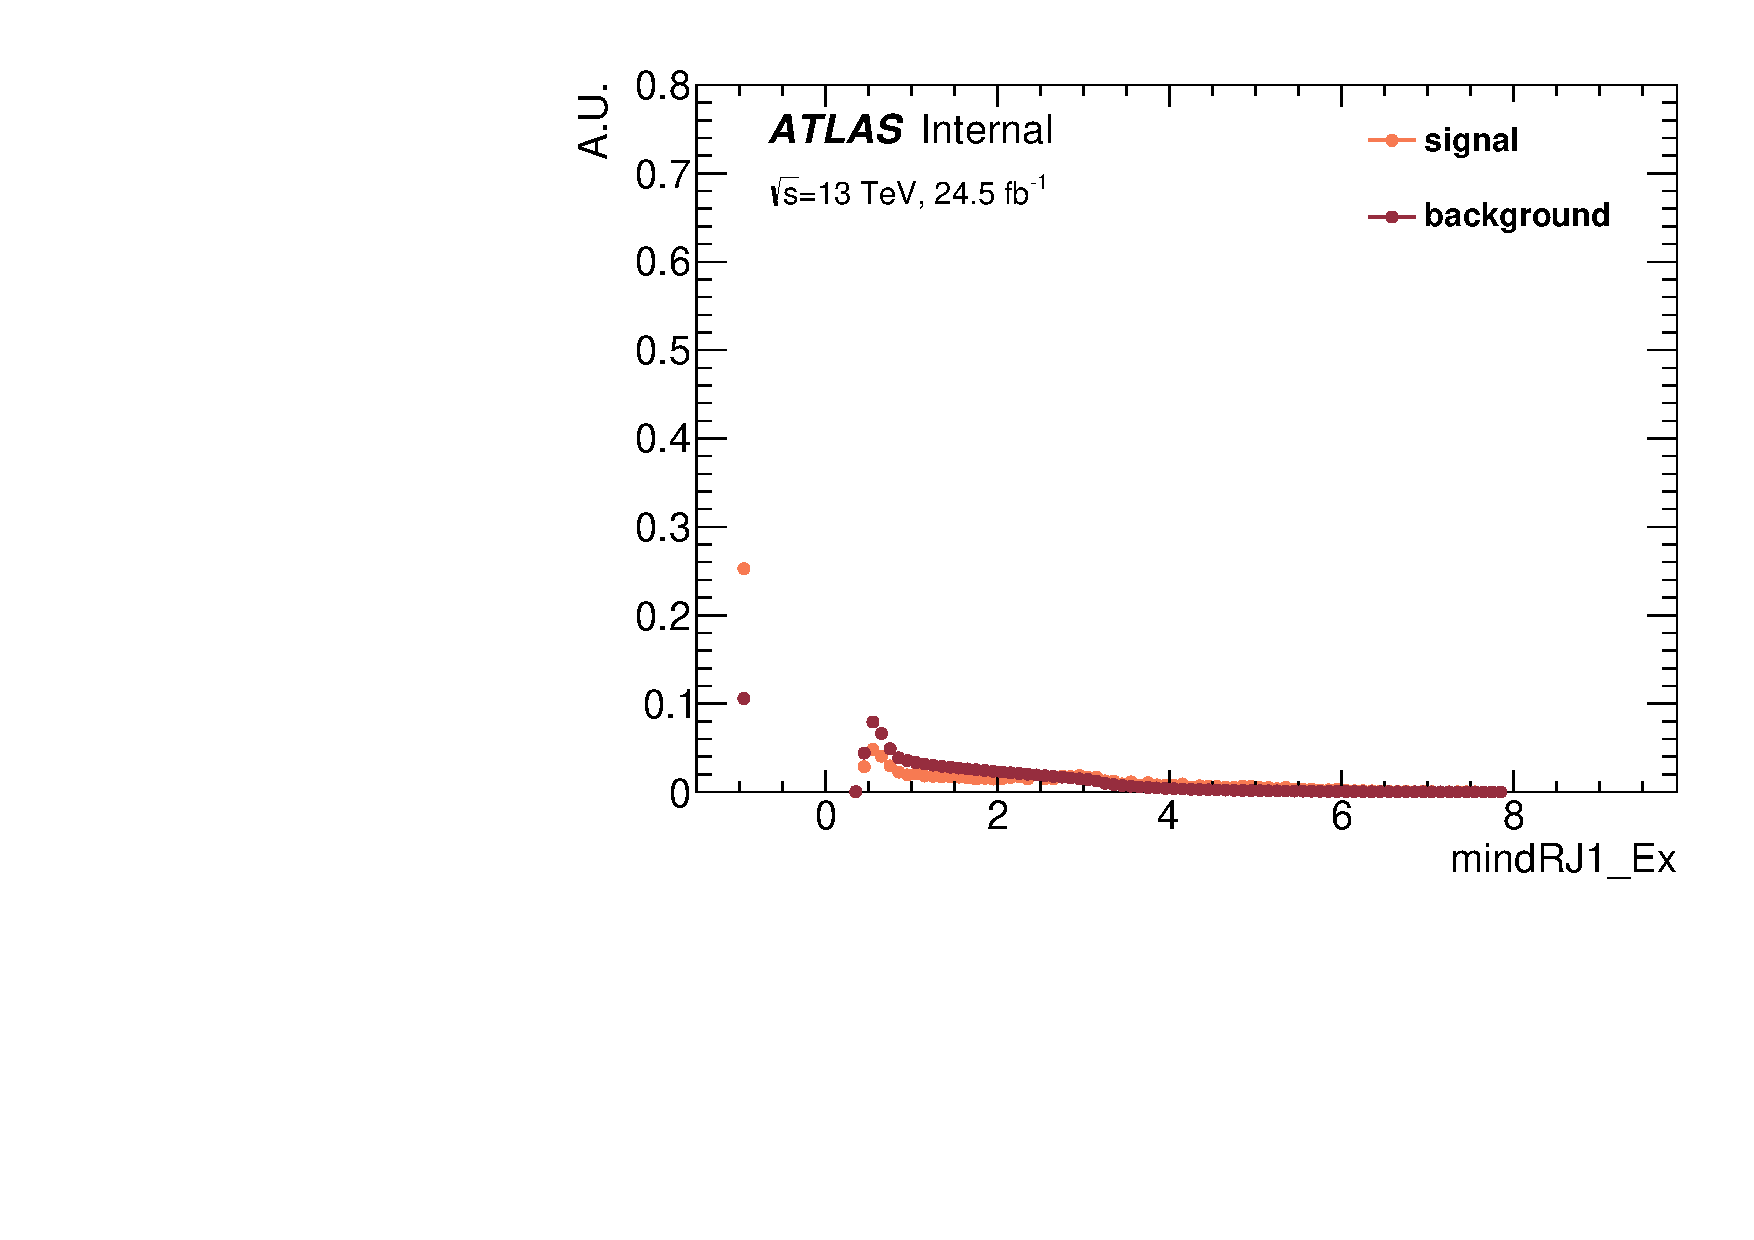
\includegraphics[width=0.3\textwidth]{figures/BDT_mindRJ1_4cen.pdf}
 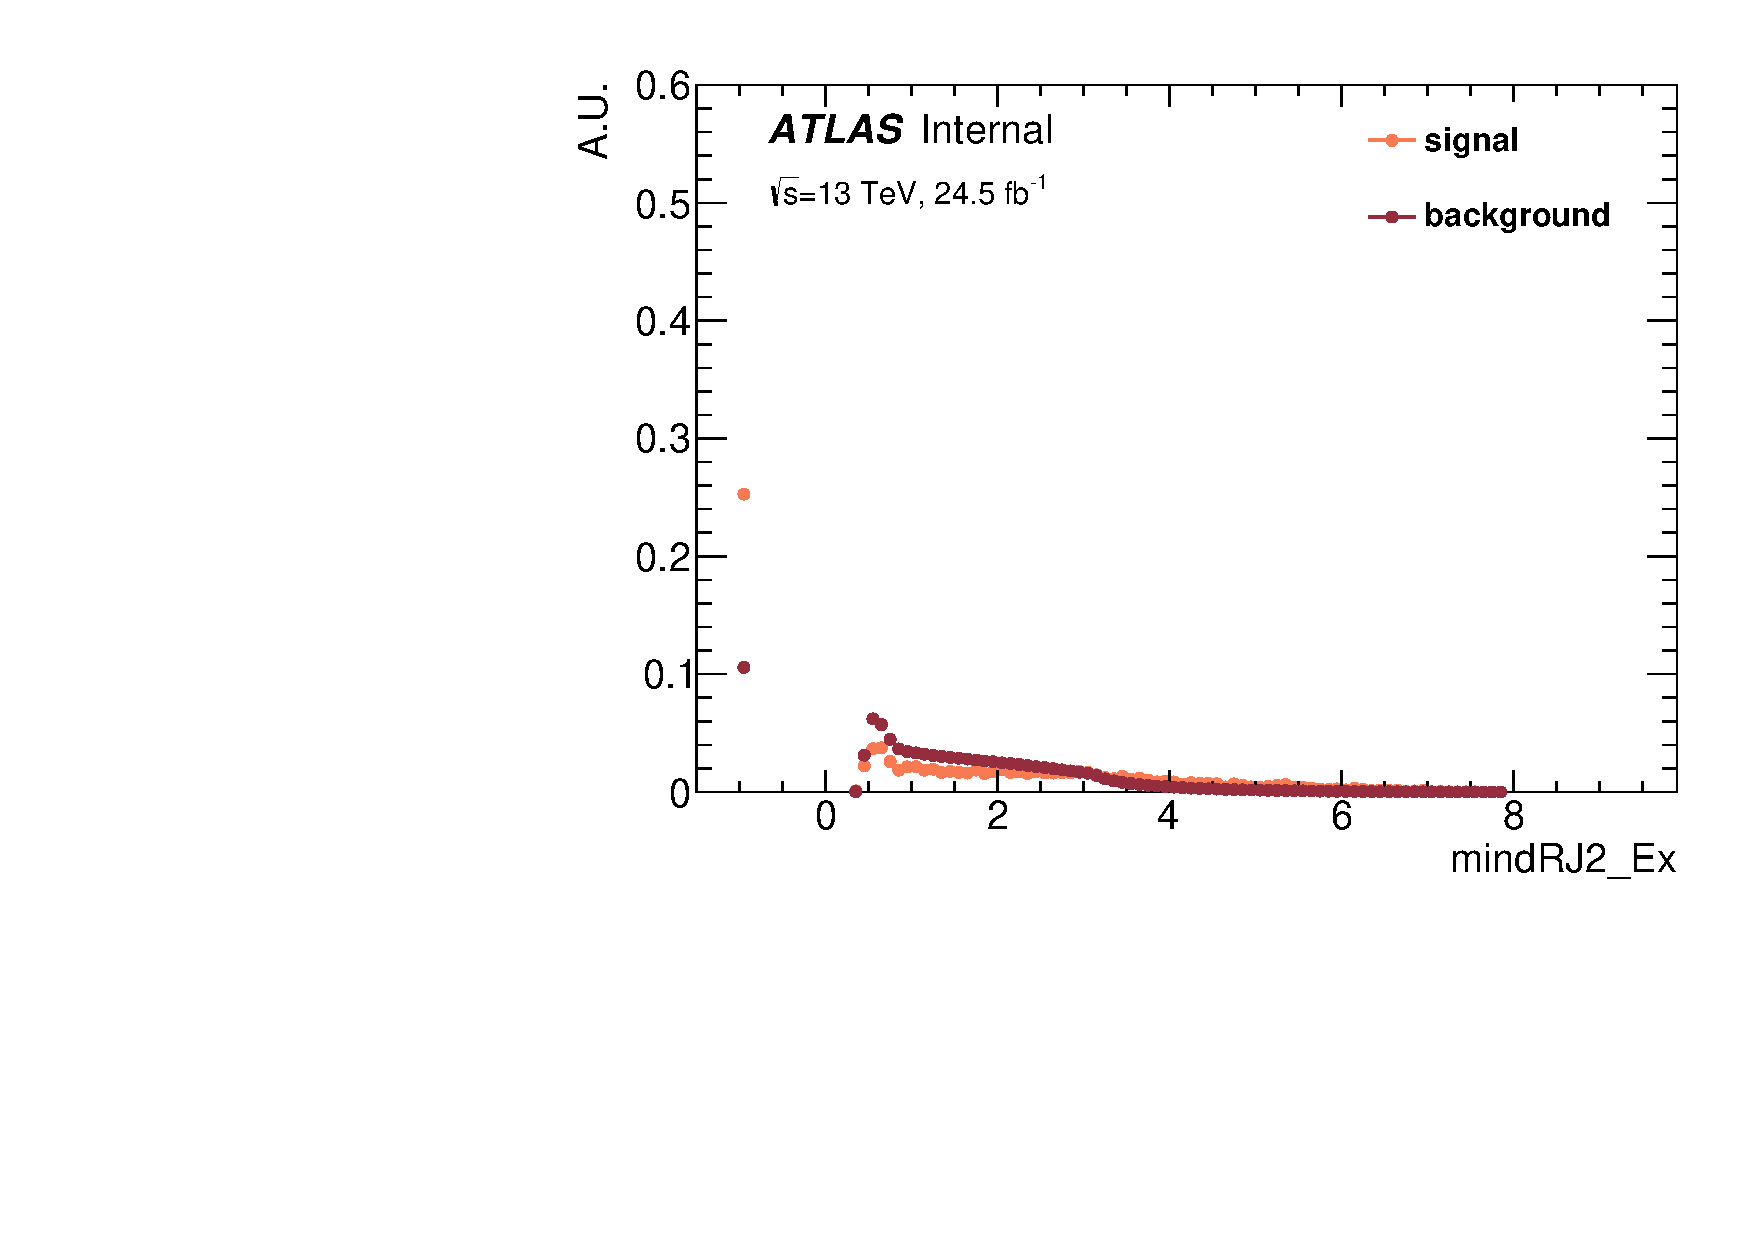
\includegraphics[width=0.3\textwidth]{figures/BDT_mindRJ2_4cen.pdf}
 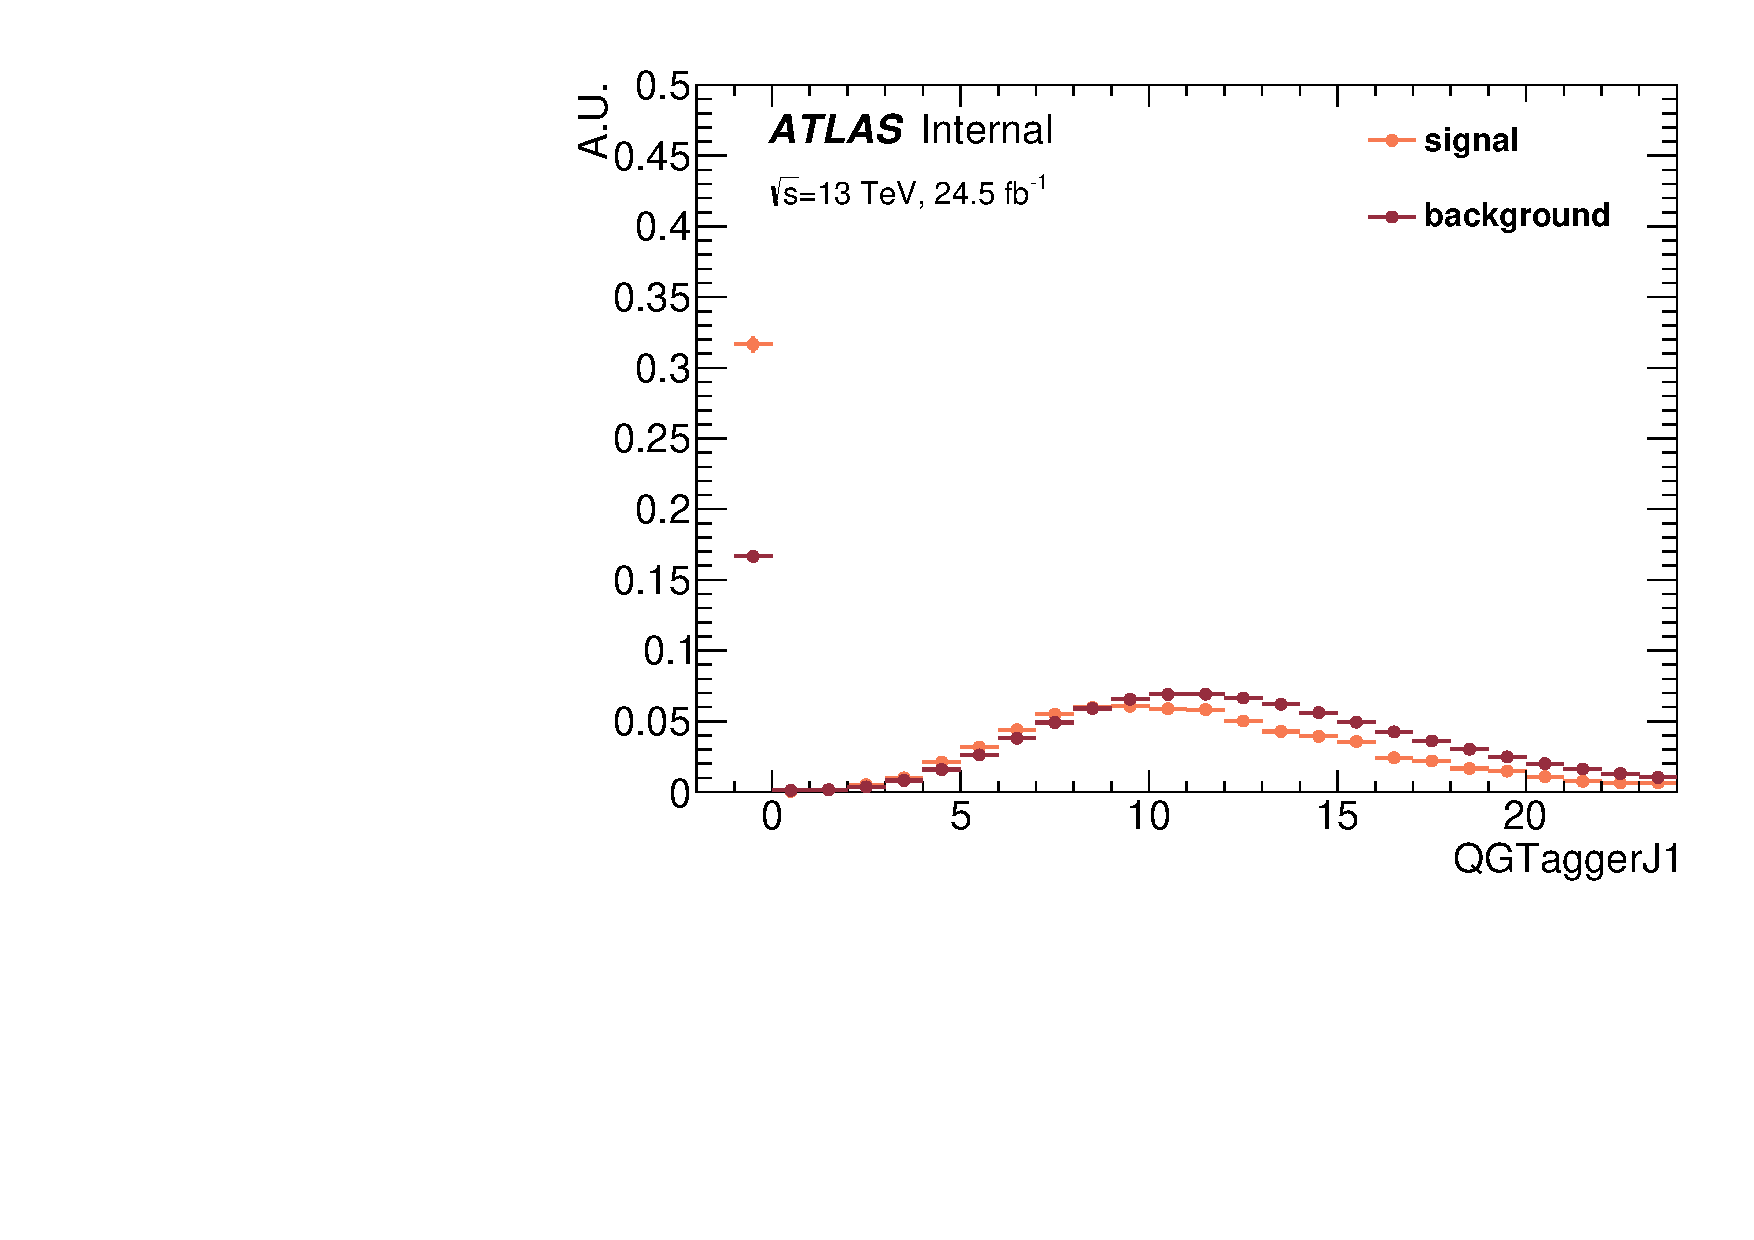
\includegraphics[width=0.3\textwidth]{figures/BDT_NTrk500_J1_4cen.pdf}\\
 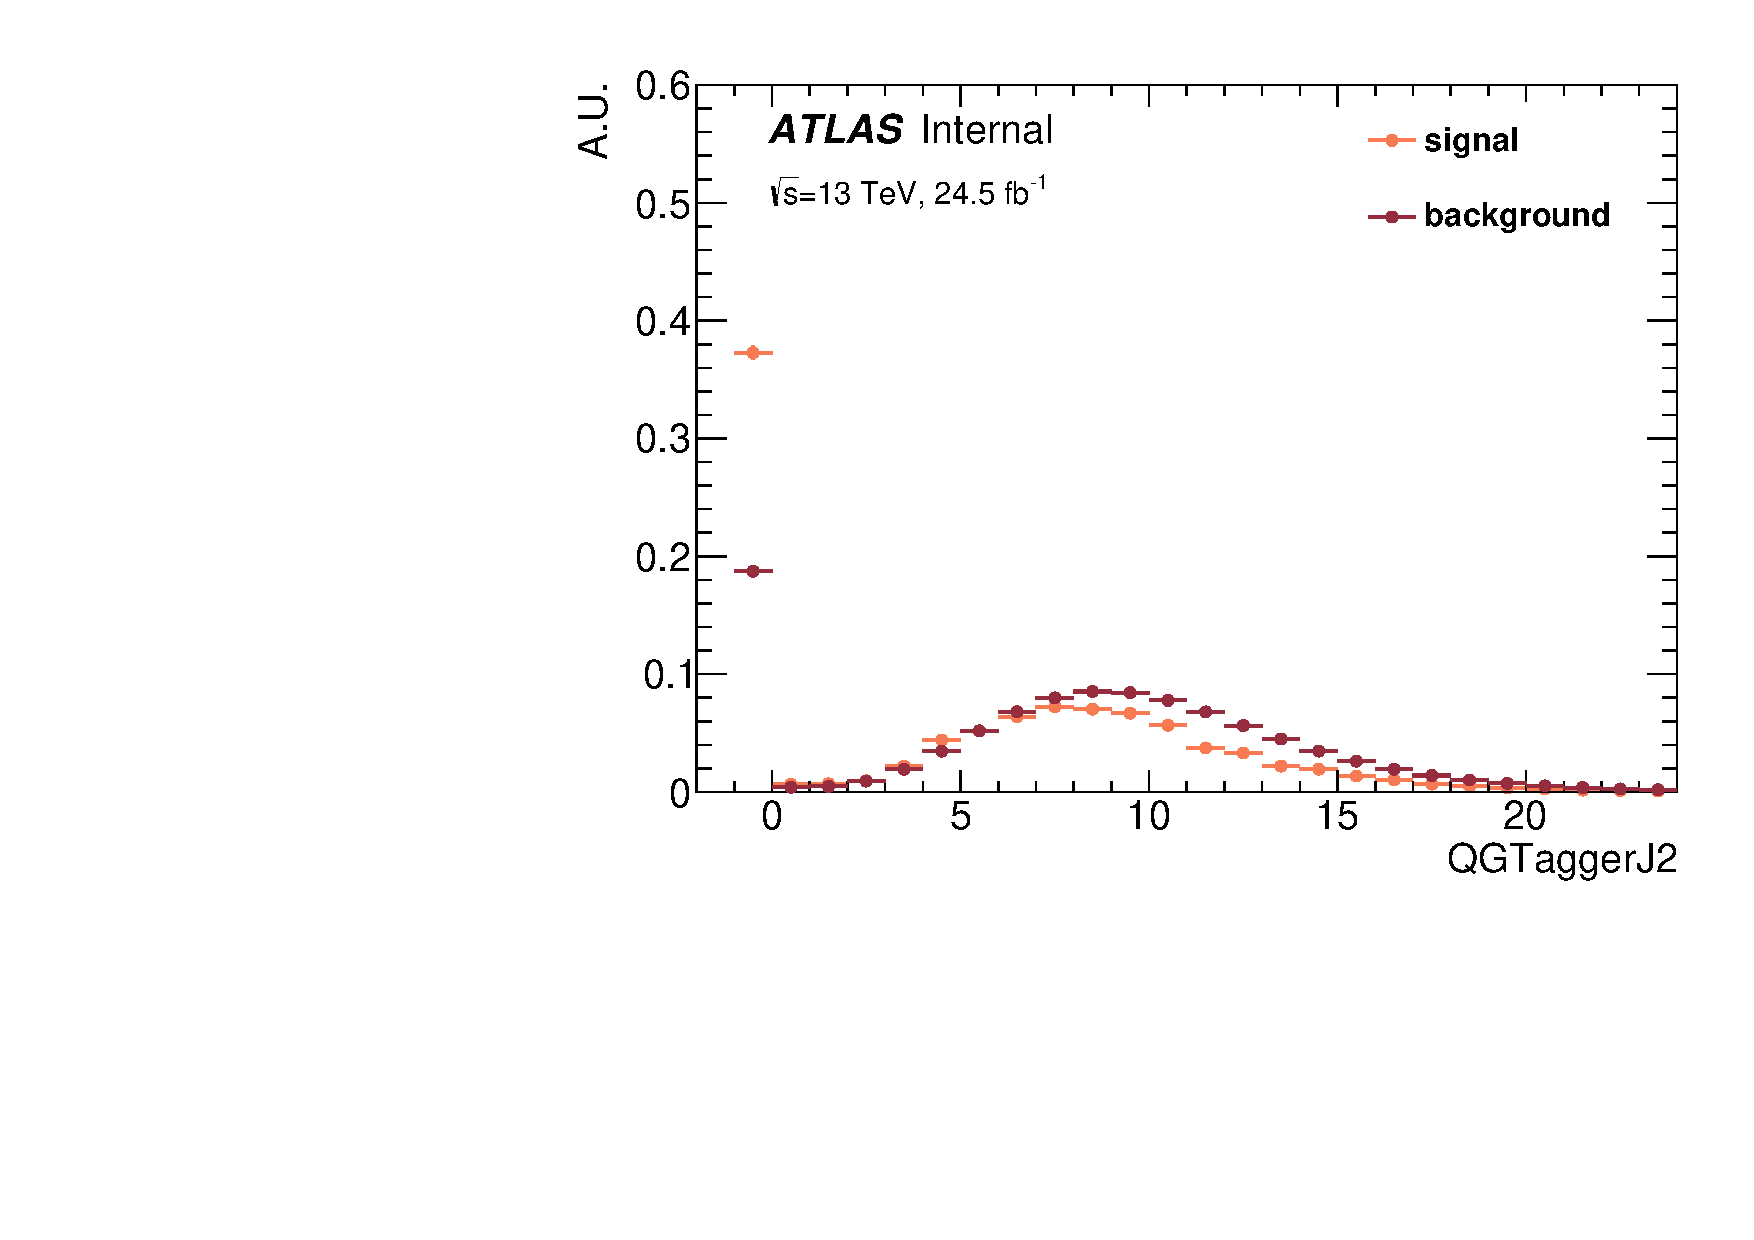
\includegraphics[width=0.3\textwidth]{figures/BDT_NTrk500_J2_4cen.pdf}
 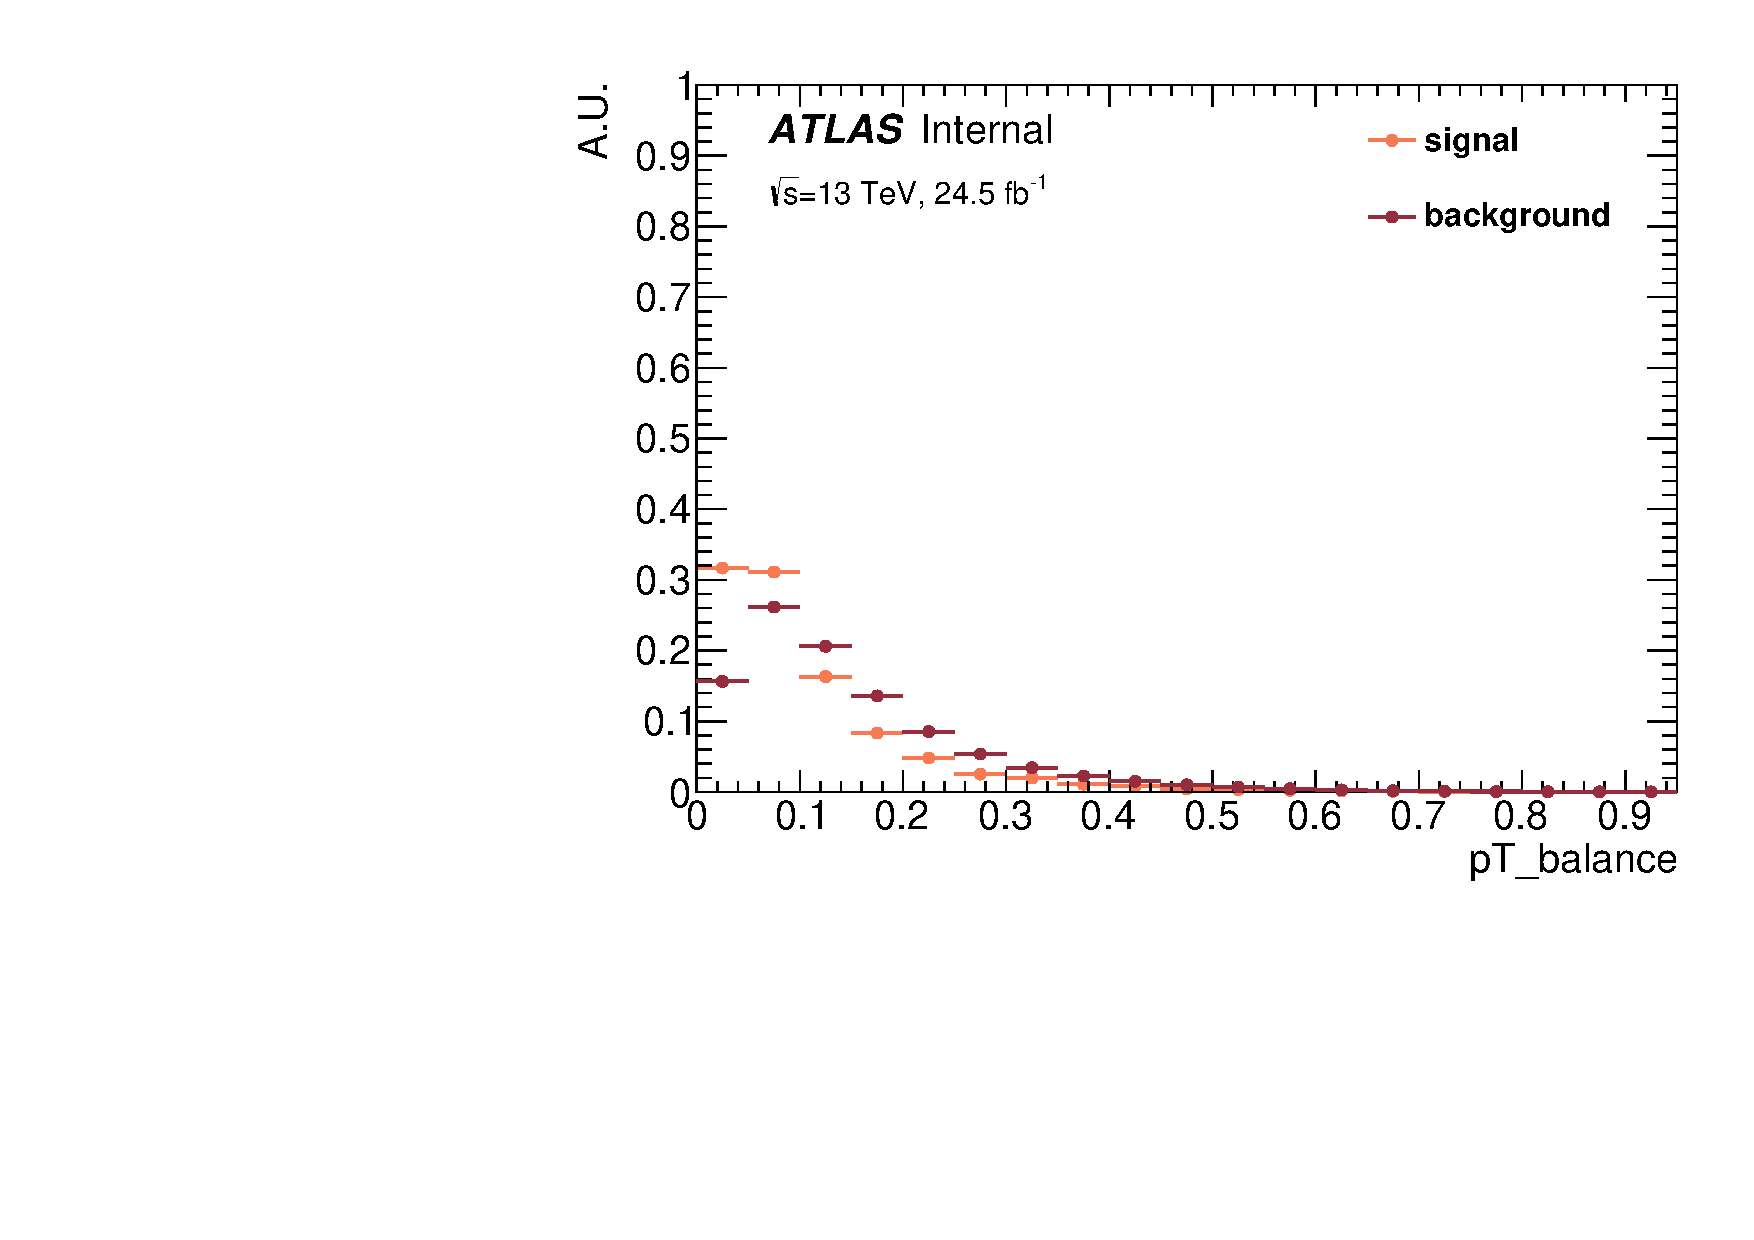
\includegraphics[width=0.3\textwidth]{figures/BDT_pTBalance_4cen.pdf}\\

 %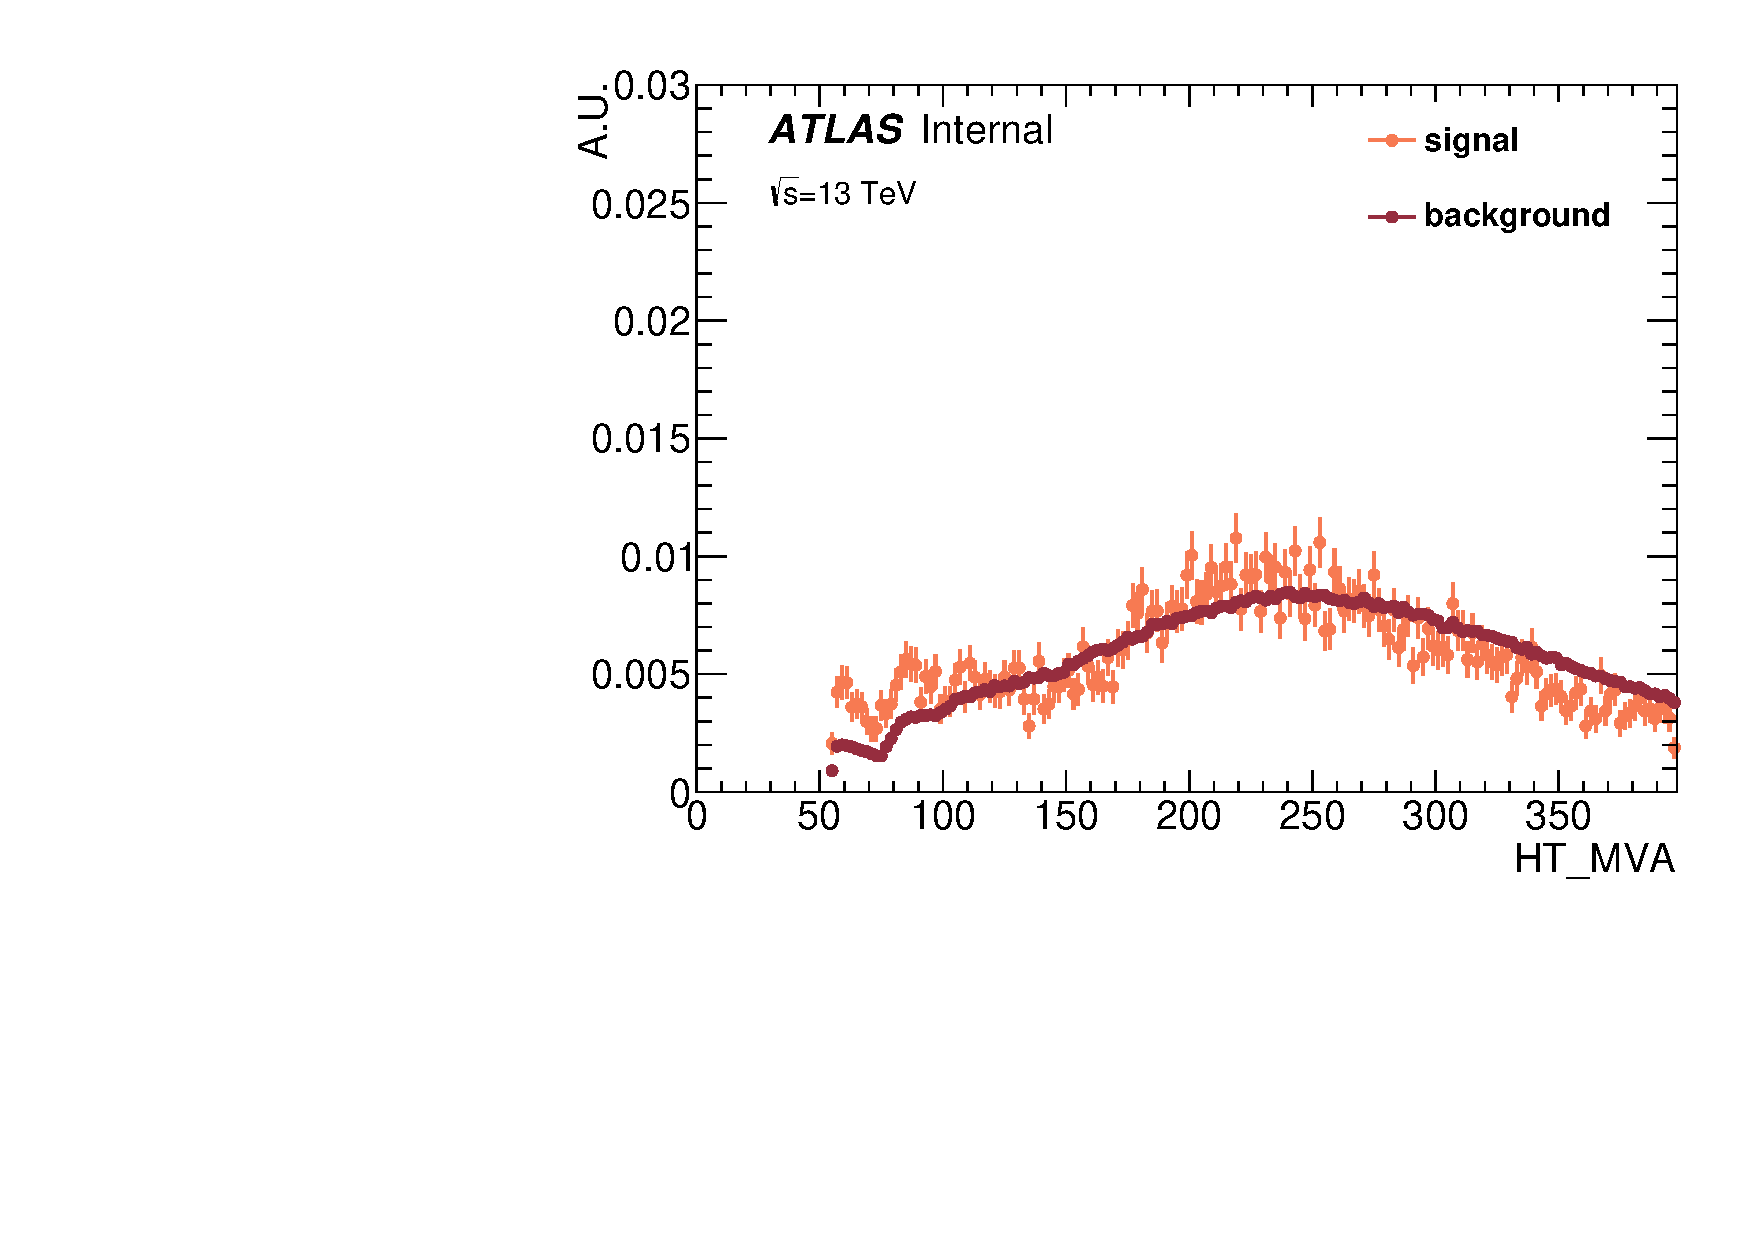
\includegraphics[width=0.3\textwidth]{figures/BDT_HT_4cen.pdf}
\caption{Distributions of BDT input variables of \fourcentral channel}
  \label{fig:BDTInputs4cen}
\end{figure}


\begin{figure}[htbp]
  \centering
 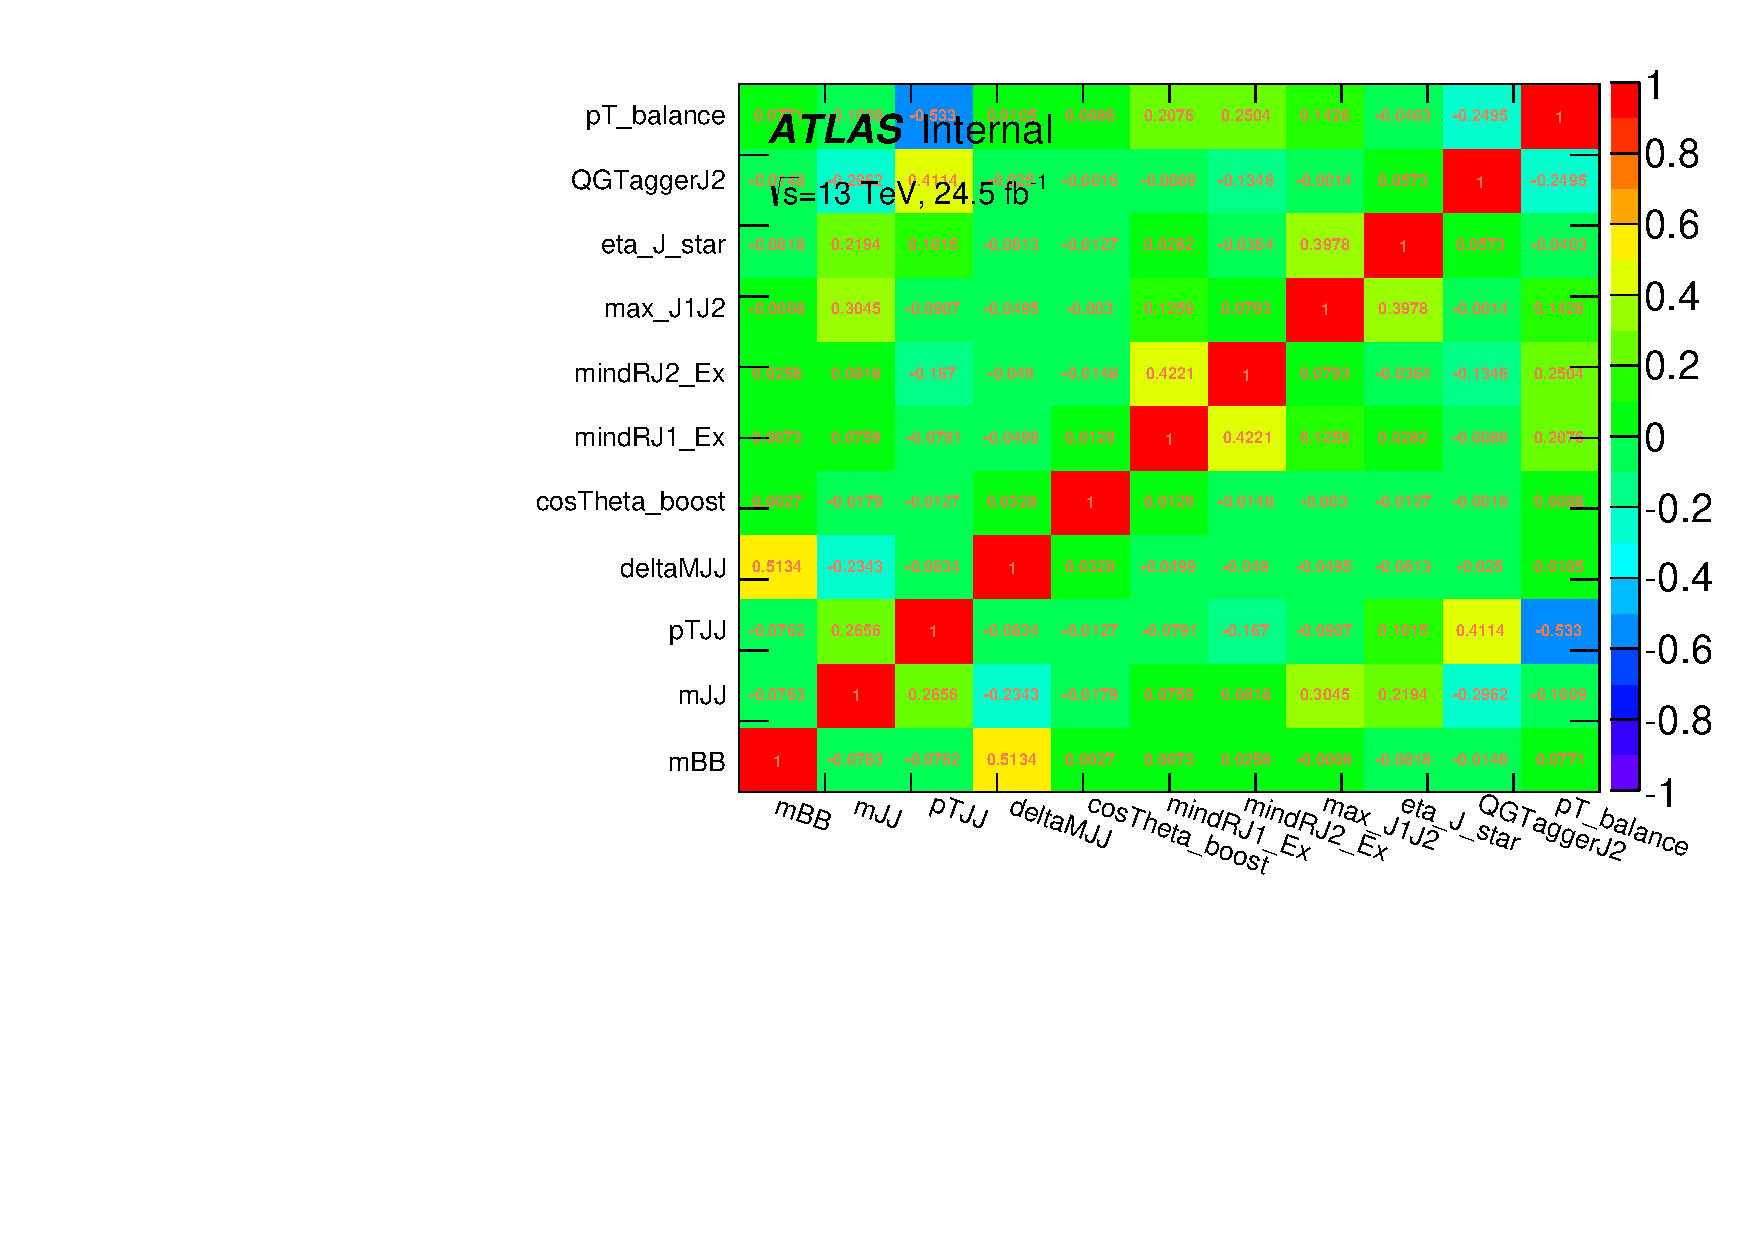
\includegraphics[width=0.48\textwidth]{figures/BDT_VBF_var_cor_2cen.pdf}
 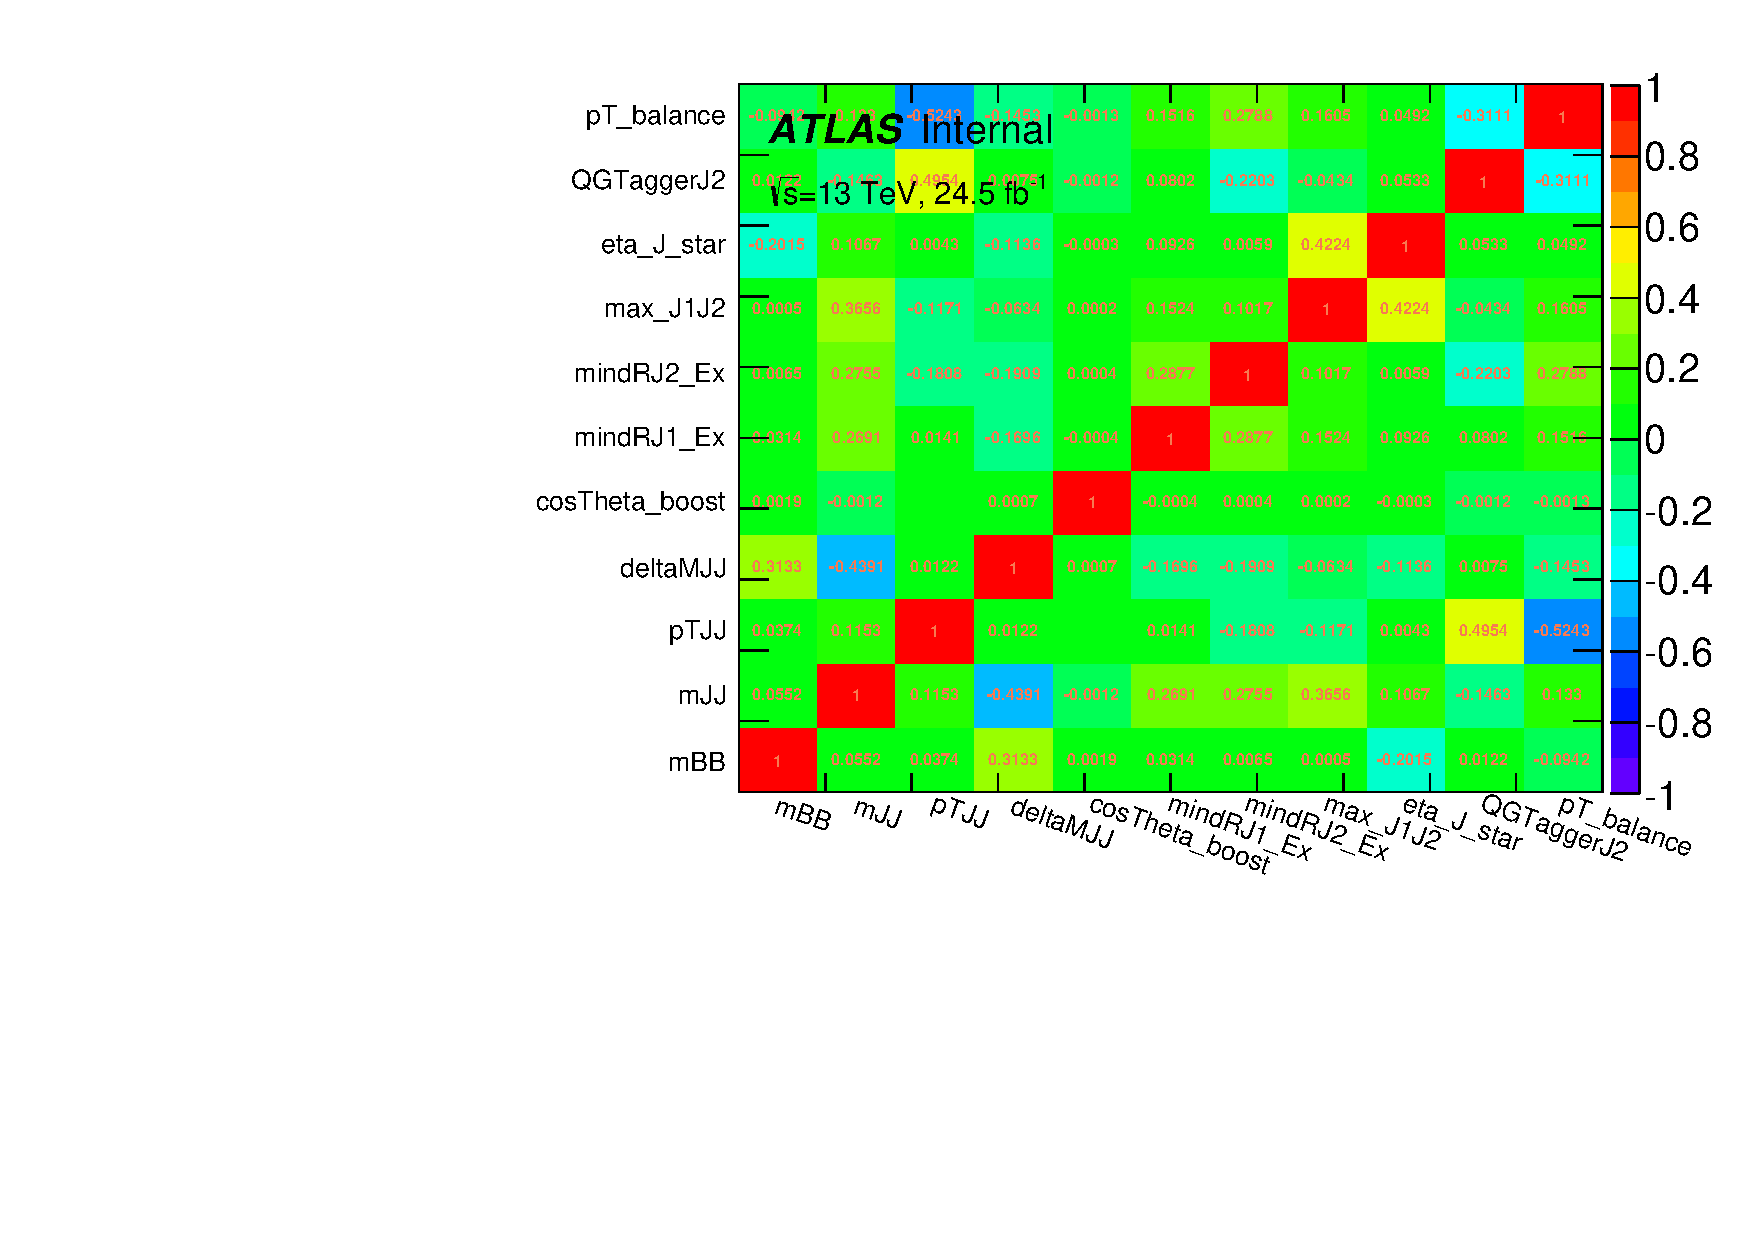
\includegraphics[width=0.48\textwidth]{figures/BDT_data_var_cor_2cen.pdf}\\
 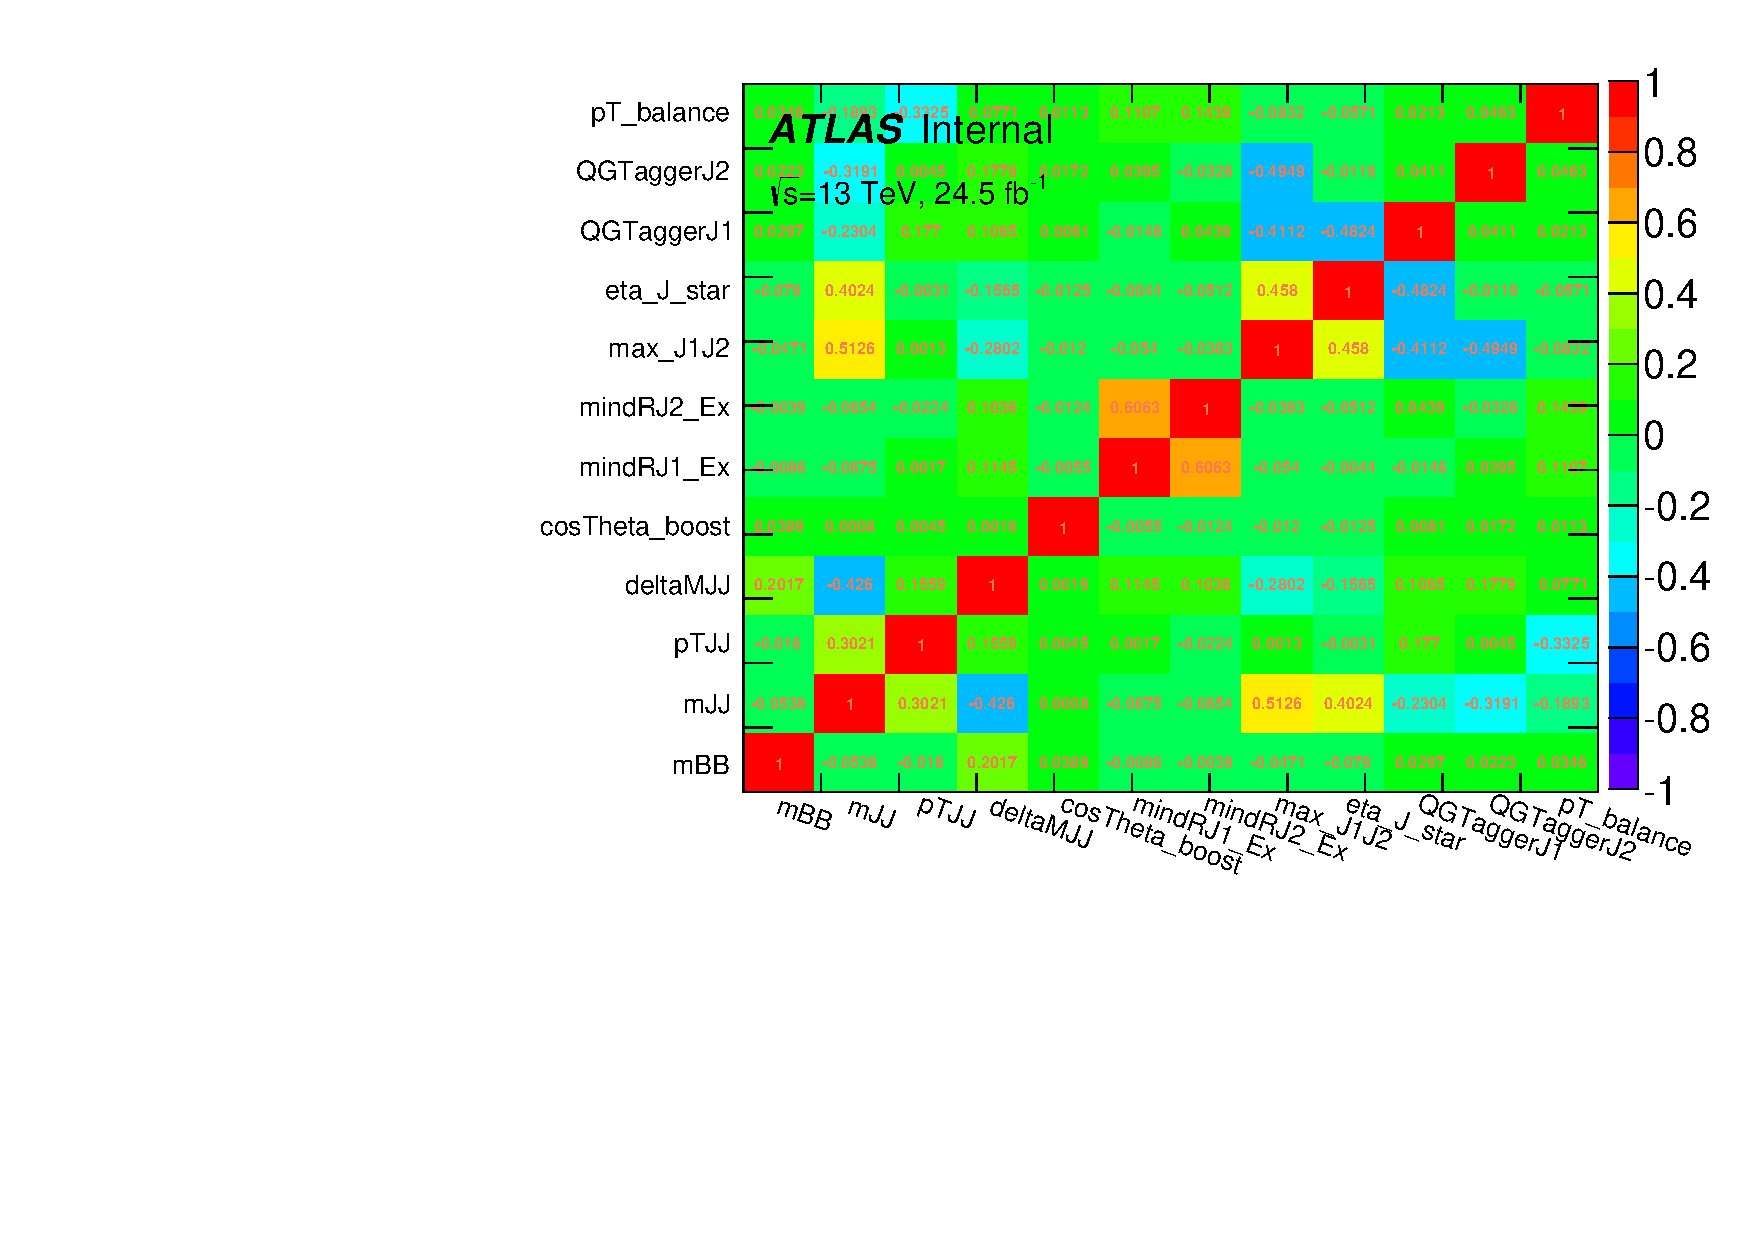
\includegraphics[width=0.48\textwidth]{figures/BDT_VBF_var_cor_4cen.pdf}
 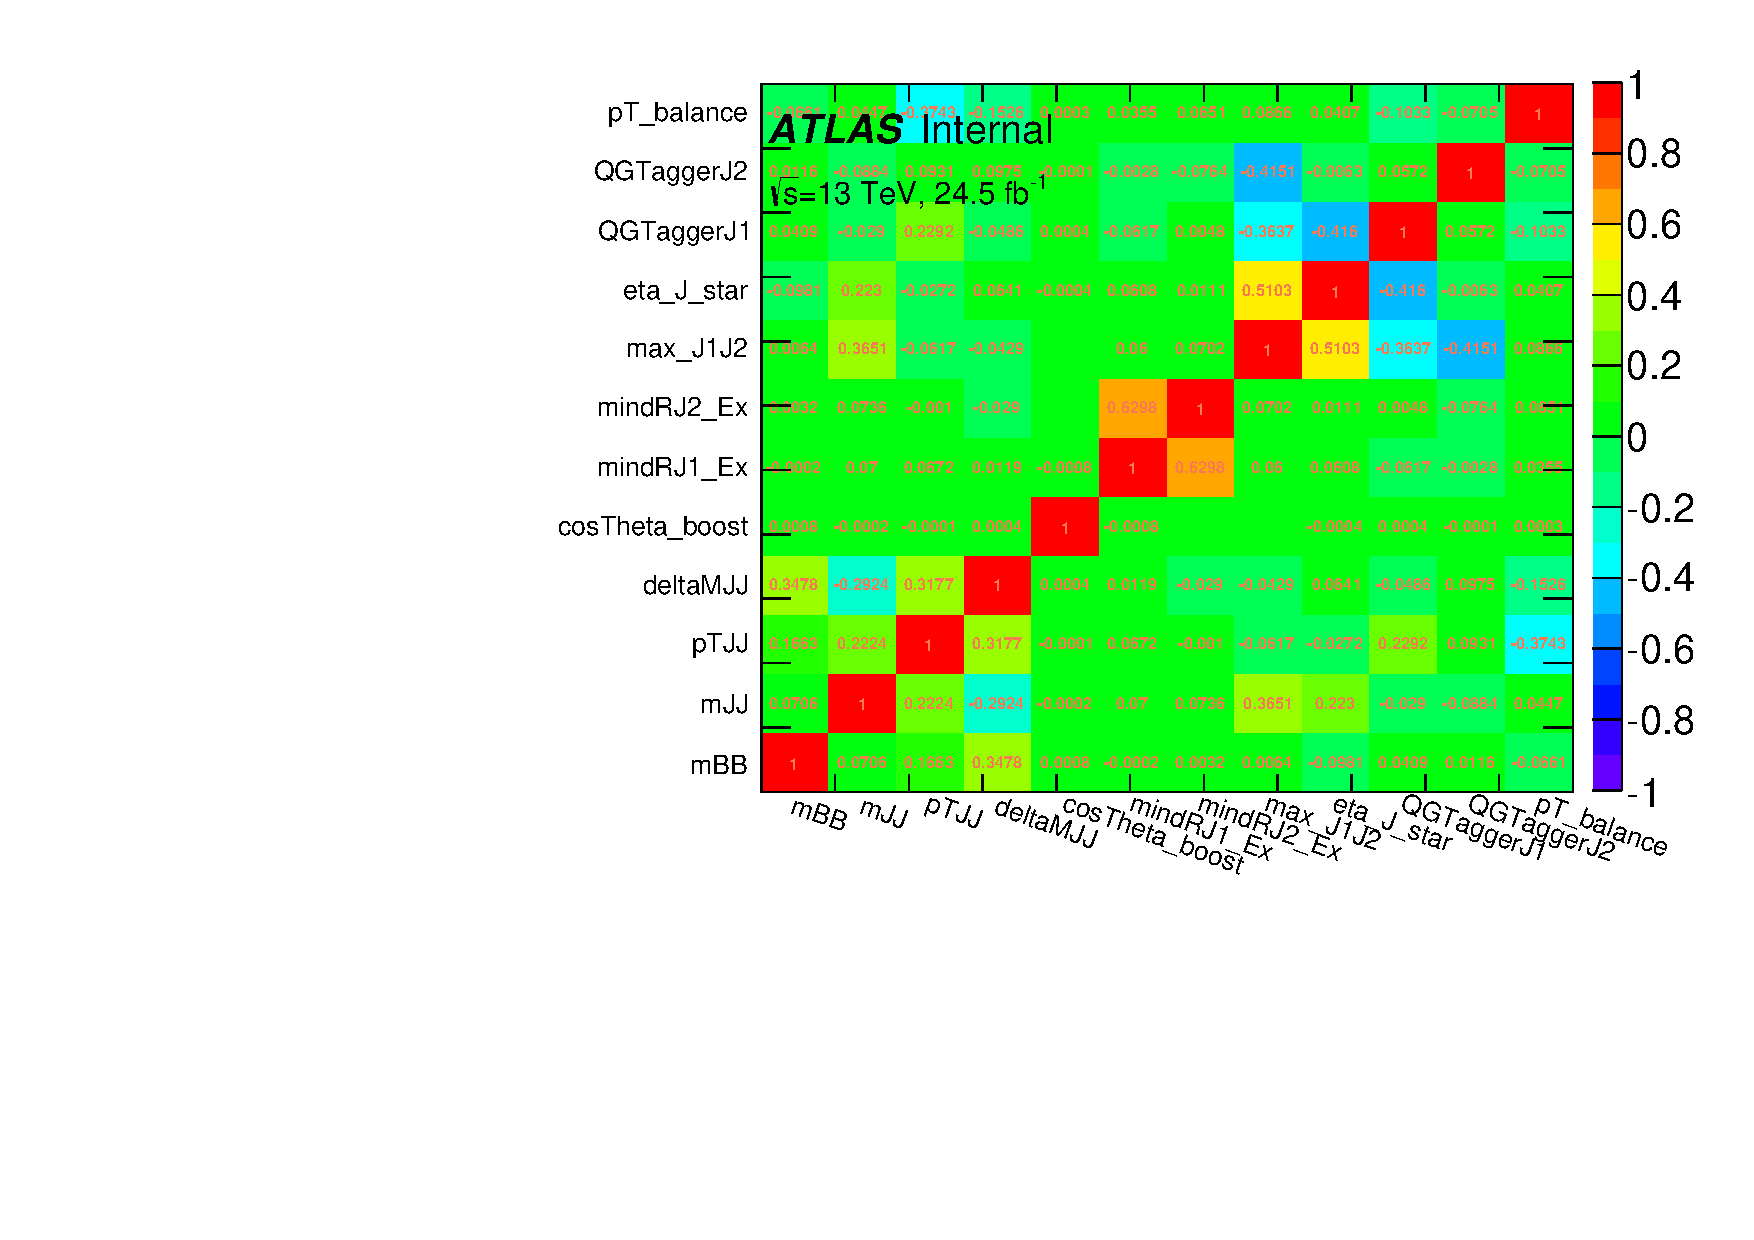
\includegraphics[width=0.48\textwidth]{figures/BDT_data_var_cor_4cen.pdf}\\
\caption{Correlations between BDT input variables and $\Mbb$ of signal (left) and background (right) of  the \twocentral (top) and \fourcentral (bottom) channels.}
  \label{fig:BDTInputsCor}
\end{figure}

\begin{figure}[htbp]
  \centering
 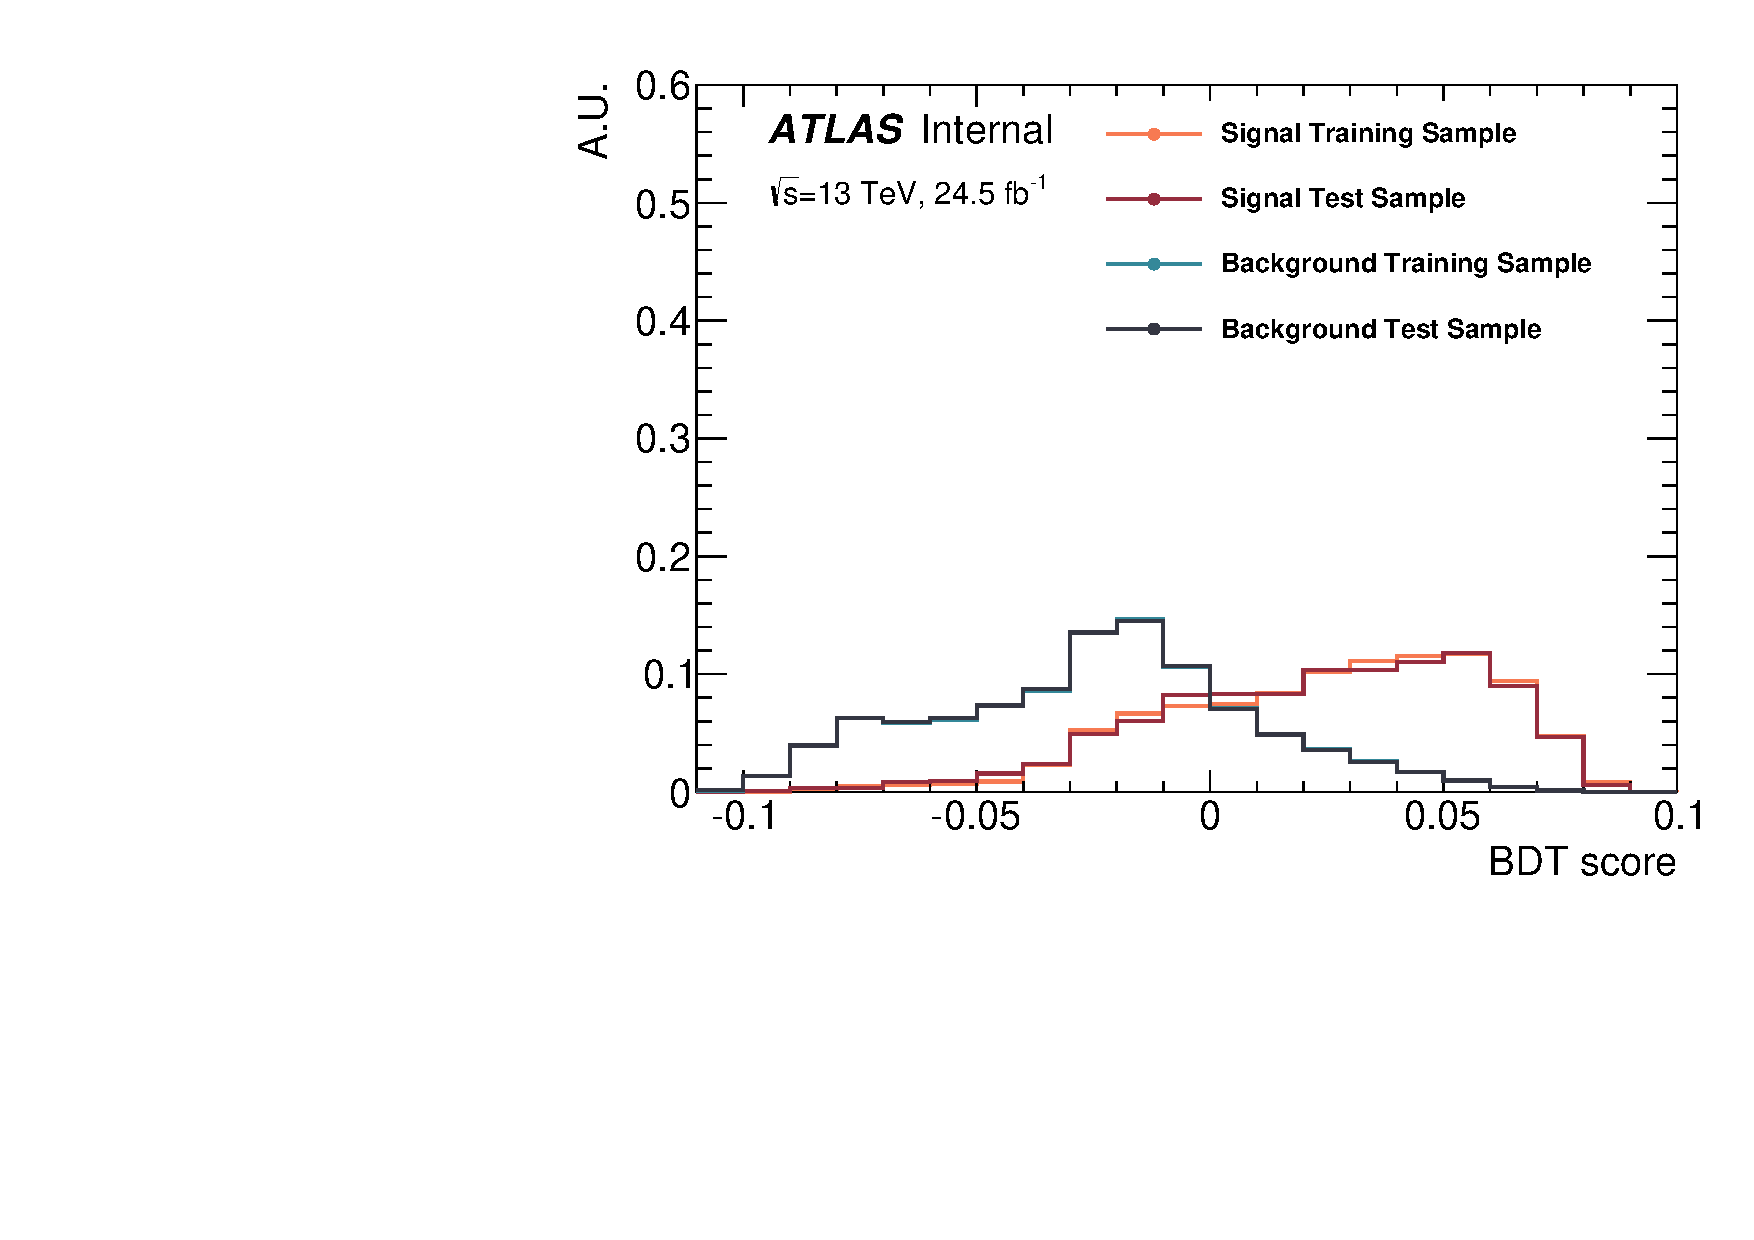
\includegraphics[width=0.48\textwidth]{figures/BDT_score_2cen.pdf}
 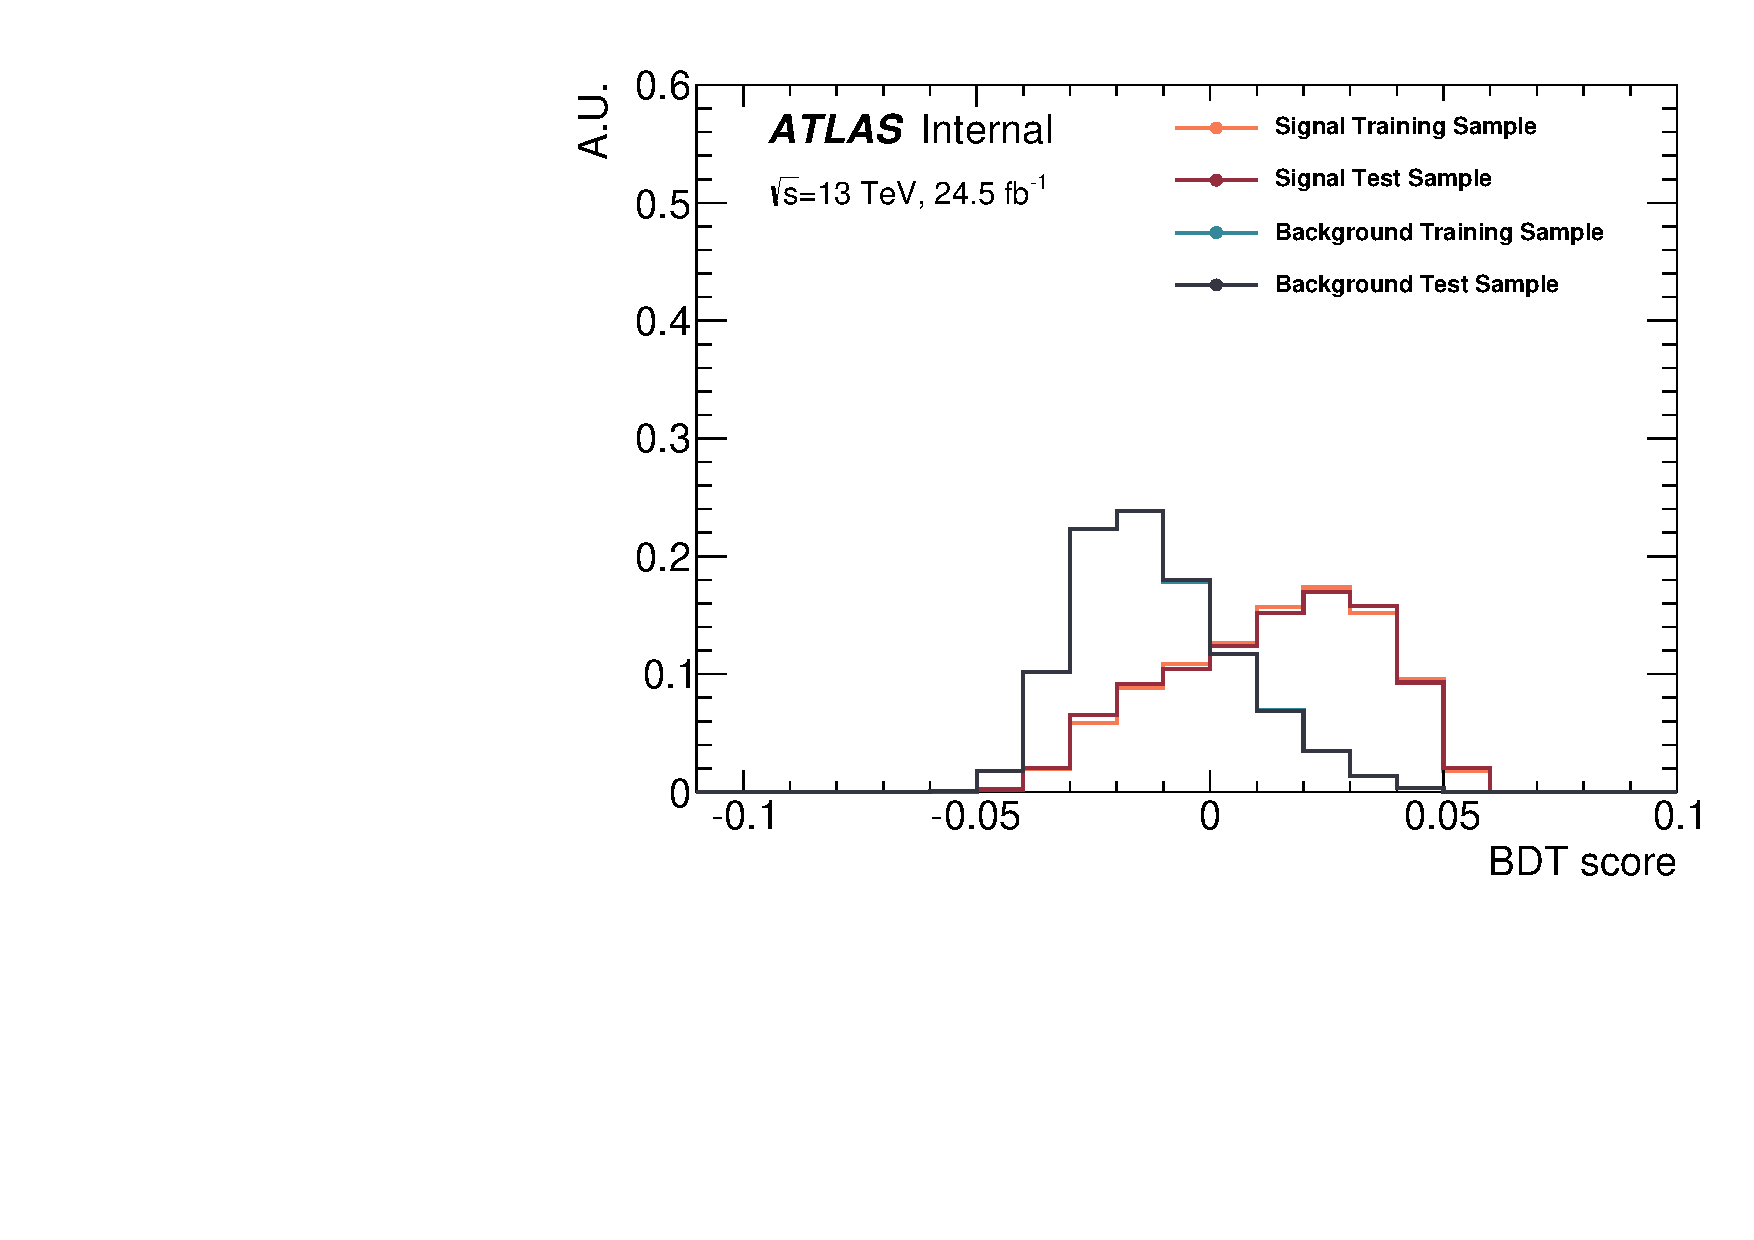
\includegraphics[width=0.48\textwidth]{figures/BDT_score_4cen.pdf}\\
 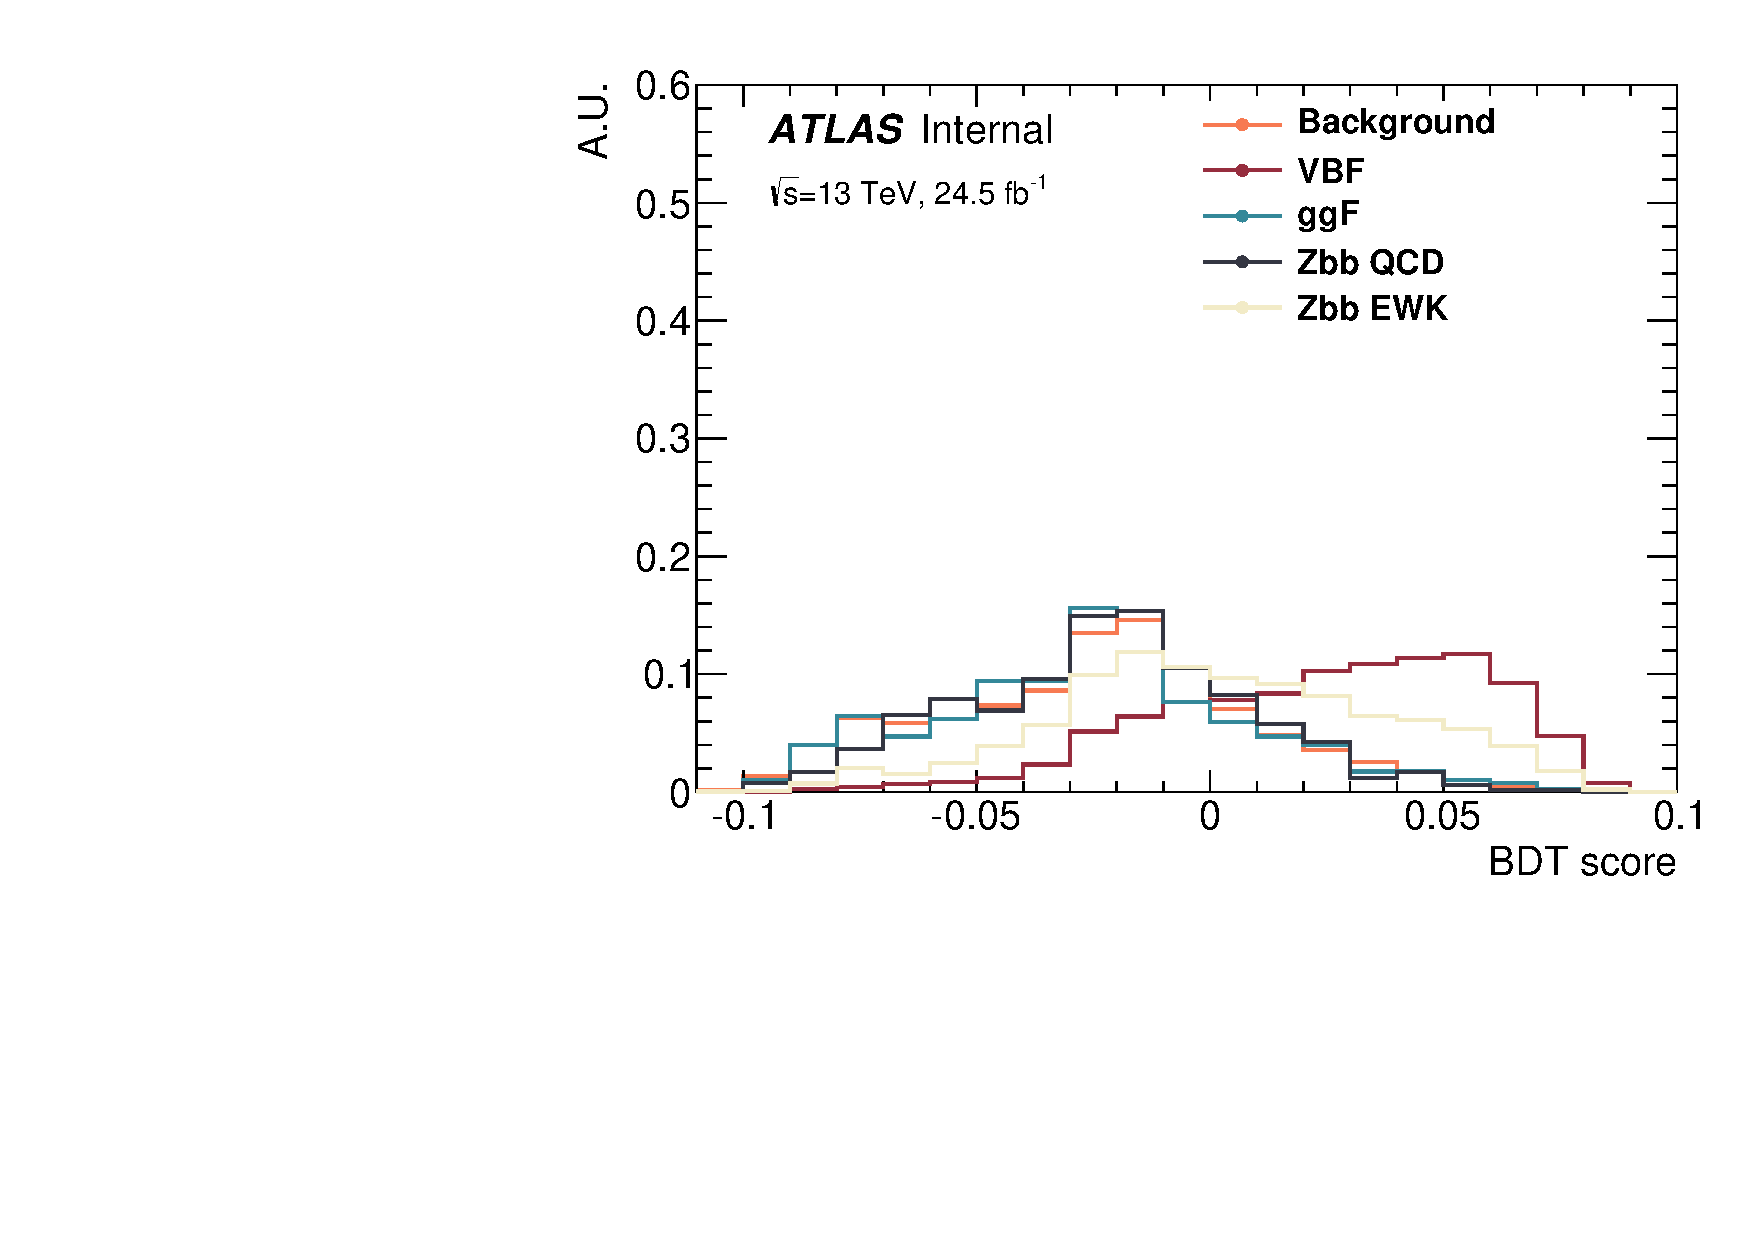
\includegraphics[width=0.48\textwidth]{figures/BDT_score_breakdown_2cen.pdf}
 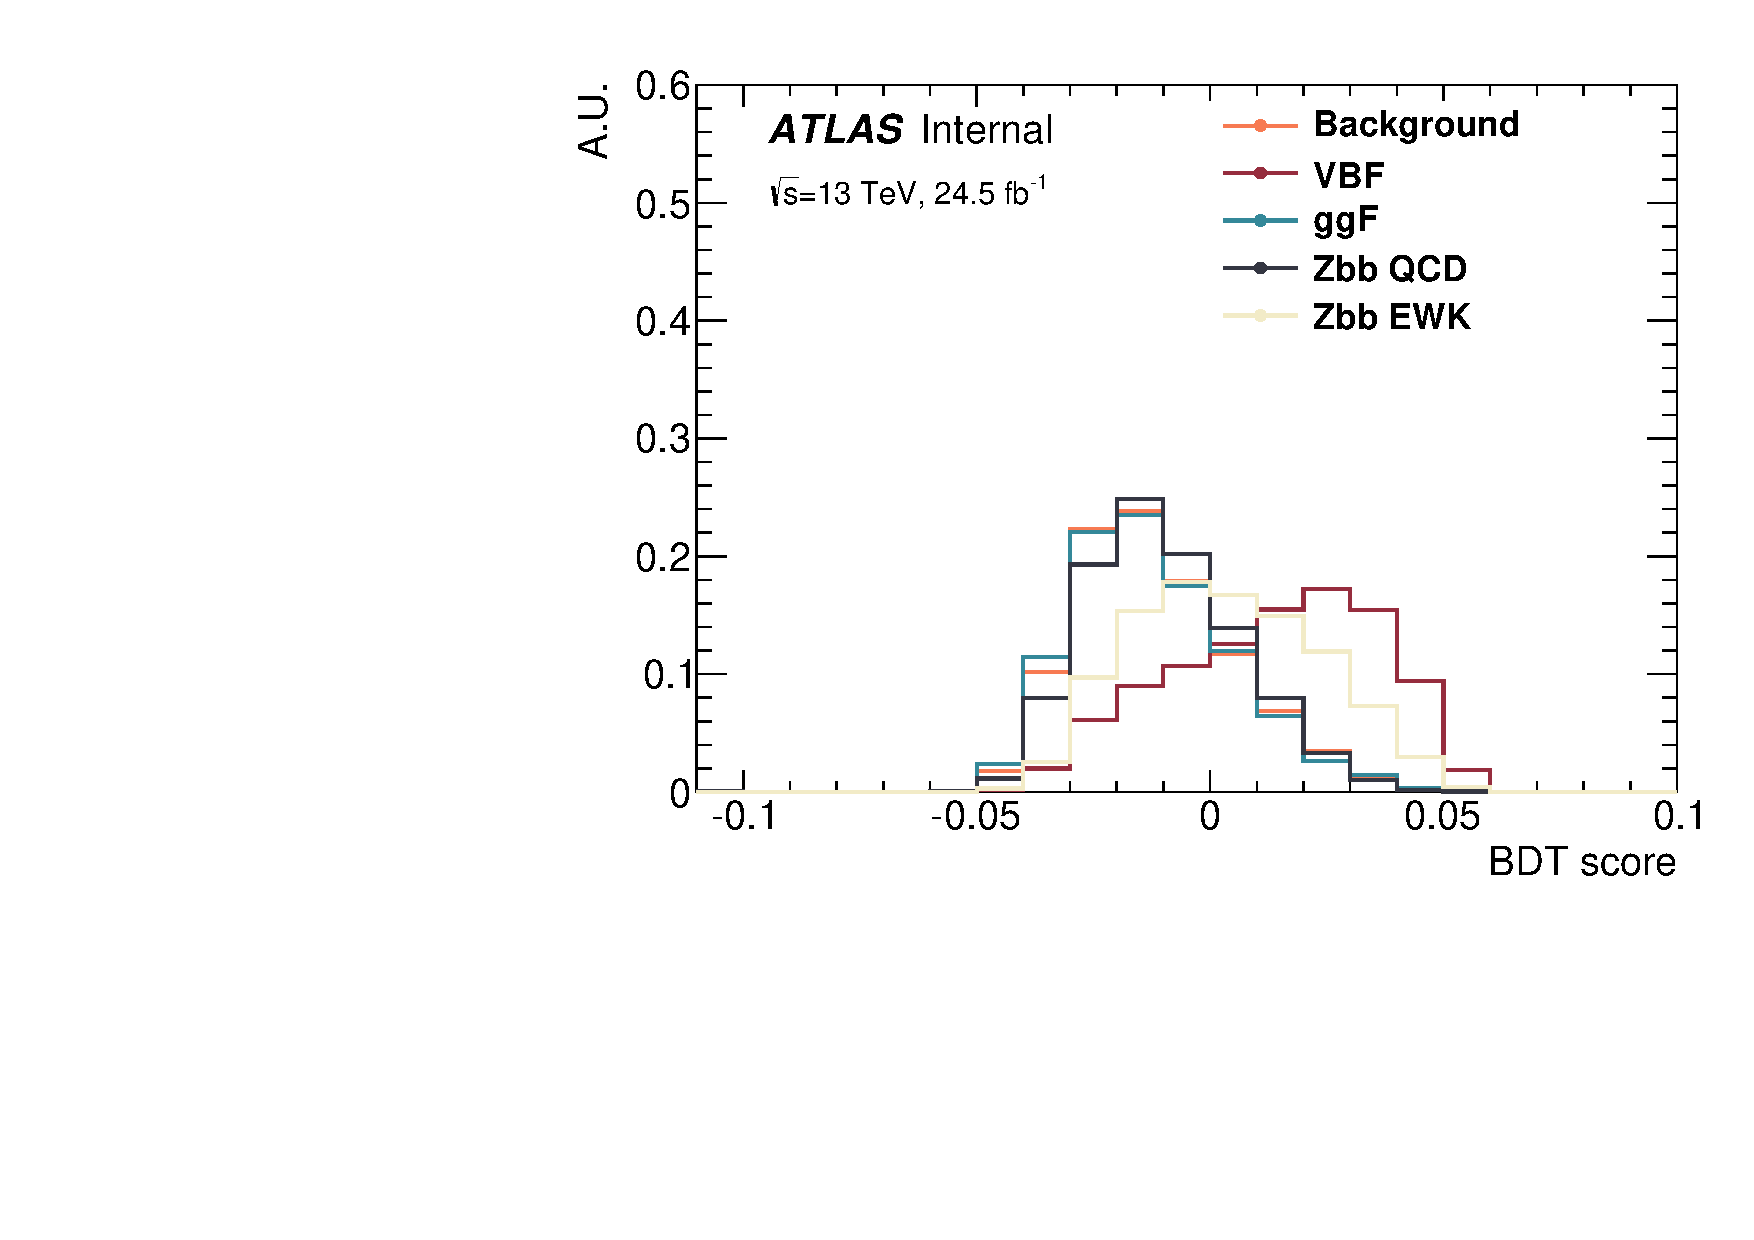
\includegraphics[width=0.48\textwidth]{figures/BDT_score_breakdown_4cen.pdf}\\
\caption{BDT Response for  the \twocentral (left) and \fourcentral (right) channel.  The top row shows the response for both the training and validation samples.  The bottom row shows a comparison of response for the signal, multijet background, $ggF$ Higgs and $Z$ boson samples. }
  \label{fig:BDTResponse}
\end{figure}


\begin{table}[]
\centering
\caption{Signal and control region definitions, yields and sensitivities for the \twocentral channel. }
\label{tab:BDTReg2cen}
\begin{tabular}{|l|l|l|l|l|}
\hline
Region          & SR I               & SR II               & SR III             & CR                    \\ \hline
BDT Score Range & \textgreater0.046  & {[}0.037, 0.046{]}  & {[}0.018, 0.037{]} & \textless-0.04        \\ \hline
\multicolumn{5}{|c|}{Total Yield}                                                        \\ \hline
QCD $Z$ & $50.78 \pm 18.50$ & $27.15 \pm 12.43$ & $193.09 \pm 40.50$   &  $894.99 \pm 84.80$    \\ \cline{2-5} 
EWK $Z$&  $15.96 \pm 1.09$ &  $8.00 \pm 0.88$  & $17.73 \pm 1.18$  &  $13.35 \pm 1.06$    \\ \hline

\multicolumn{5}{|c|}{Sideband}  \\ \hline
Non-resonant (sideband low)     & $1781 \pm 42.20$  & $1481 \pm 38.48 $ & $5171 \pm 71.91$ & $25992 \pm 161.22$    \\ \cline{2-5} 
Non-resonant (sideband high)    & $2974 \pm 54.53$  & $2574 \pm 50.73 $ & $8866 \pm 94.16$ & $43051 \pm 207.49$    \\ \hline

\multicolumn{5}{|c|}{Yield in Higgs Mass Window}                                                        \\ \hline
VBF             & $40.50 \pm 0.48$   & $12.62\pm 0.51$     & $23.87\pm 0.72$    & $2.61 \pm 0.18$       \\ \cline{2-5} 
ggF             & $3.13 \pm 0.10$    & $1.11\pm 0.16$      & $5.38\pm 0.30$     & $28.26\pm 0.60$       \\ \cline{2-5}
No-resonant (extrapolated)    & $2466.82 \pm 49.67$ & $2364.68 \pm 48.63$ & $7240.39\pm 85.09$ & $38117.09 \pm 195.24$ \\ \hline
\multicolumn{5}{|c|}{Expected Sensitivity}                                                              \\ \hline
$S/ \sqrt(B)$   & 0.88               & 0.30                & 0.33               & 0.15                  \\ \hline
\end{tabular}
\end{table}


\begin{table}[]
\centering
\caption{Signal and control region definitions, yields and sensitivities for the \fourcentral channel. }
\label{tab:BDTReg4cen}
\begin{tabular}{|l|l|l|l|}
\hline
Region              & SR I       & SR II     & CR    \\ \hline
\hline
BDT Score Range &  >0.039 & [0.022, 0.039]   & <-0.033 \\ \hline

\multicolumn{4}{|c|}{Total Yield}                                                        \\ \hline
QCD $Z$  & $342.52 \pm 65.08$   &  $1444.29 \pm 106.55$  & $2223.93 \pm 122.32$     \\ \cline{2-4} 
EWK $Z$  & $65.85 \pm 1.78$   &  $73.94 \pm 1.89$ &    $10.59 \pm 0.66$  \\ \hline

\multicolumn{4}{|c|}{Sideband}  \\ \hline
Non-resonant (sideband low)   & $ 7884 \pm 88.79$  & $26059 \pm 161.43 $ & $50004 \pm 223.62  $    \\ \cline{2-4} 
Non-resonant (sideband high)  & $ 11244 \pm 106.04$  & $34136 \pm 184.76 $ & $72620 \pm 269.48 $   \\ \hline

\multicolumn{4}{|c|}{Yield in Higgs Mass Window} \\
\hline
VBF                     & $49.50\pm 0.80$                  & $ 47.06\pm 0.78$                 & $1.96 \pm 0.16$                    \\ \hline
ggF                     & $8.02 \pm 0.32$                  & $27.70 \pm 0.60$                 & $75.3 \pm 0.99$                    \\ \hline
%Zbb QCD                 & 1.44                  & 17.30                 & 56.76                   \\ \hline
%Zbb EWK                 & 0.21                  & 0.98                  & 0.43                    \\ \hline
No-resonant (extrapolated) & $6974.30 \pm 83.51$                & $31640.83 \pm 177.88$               &  $80625.16 \pm 283.95$                  \\ \hline
\hline 
\multicolumn{4}{|c|}{Expected Sensitivity} \\
\hline
$S/ \sqrt(B)$           & 0.69                  & 0.39                  & 0.27                    \\ \hline
\end{tabular}
\end{table}
